\documentclass[11pt]{report}

% === Core Packages (order matters) ===
\usepackage[english]{babel}
\usepackage[utf8]{inputenc}
\usepackage[T1]{fontenc}

% === Fonts ===
\usepackage[sfdefault]{roboto}        % Roboto as main font
\usepackage{sfmath}                    % Sans-serif math fonts for consistency
% Note: Using bold Roboto for headers instead of Roboto Slab (not in standard TeX Live)

% === Graphics and Colors ===
\usepackage{graphicx}
\usepackage{xcolor}
\usepackage{tikz}
\usepackage{tikzpagenodes}
\usetikzlibrary{decorations.pathreplacing, shapes.geometric, positioning}
\usepackage{tcolorbox}
\usepackage{tabularray}

% === Page Layout ===
\usepackage{geometry}
\geometry{a4paper, margin=2.5cm}

% === Typography ===
\usepackage{microtype}
\setlength\parindent{0pt}
\setlength{\parskip}{1em}

\usepackage{pythontex}



% === Section Formatting ===
\usepackage{titlesec}
\usepackage{sectsty}


% === Figures and Tables ===
\usepackage{float}
\usepackage{caption}
\usepackage{subcaption}
\usepackage{booktabs}
\usepackage{multirow}

% === Math ===
\usepackage{amsmath}
\usepackage{amssymb}

% === Code Listings ===
\usepackage{listings}

% === Bibliography ===
\usepackage[square,sort,comma,numbers]{natbib}

% === Todo Notes ===
\usepackage[colorinlistoftodos]{todonotes}

% === Title Customization ===
\usepackage{titling}
\usepackage{blindtext}

% === Hyperlinks (load near end) ===
\usepackage{hyperref}

% === TU Delft Colors ===
\definecolor{tudelftdarkblue}{RGB}{12,35,64}
\definecolor{tudelftcyan}{RGB}{0,166,214}
\definecolor{tudelftblue}{RGB}{0,118,194}

% === Code Listing Colors ===
\definecolor{darkgreen}{rgb}{0.0, 0.4, 0.0}
\definecolor{codegreen}{rgb}{0,0.5,0.1}
\definecolor{codegray}{rgb}{0.5,0.5,0.5}
\definecolor{codepurple}{rgb}{0.58,0,0.67}
\definecolor{backcolour}{rgb}{0.92,0.94,0.96}
\definecolor{keywordcolor}{rgb}{0.8, 0.2, 0.4}

% === Chapter and Section Styling ===
\titleformat{\chapter}[display]
  {\normalfont\huge\fontfamily{RobotoSlab-TLF}\bfseries\color{tudelftdarkblue}}
  {\chaptertitlename\ \thechapter}{20pt}{\Huge}

\titleformat{\section}
  {\normalfont\Large\fontfamily{RobotoSlab-TLF}\bfseries\color{tudelftdarkblue}}
  {\thesection}{1em}{}

\titleformat{\subsection}
  {\normalfont\large\fontfamily{RobotoSlab-TLF}\bfseries\color{tudelftdarkblue}}
  {\thesubsection}{1em}{}

\titleformat{\subsubsection}
  {\normalfont\normalsize\fontfamily{RobotoSlab-TLF}\bfseries\color{tudelftblue}}
  {\thesubsubsection}{1em}{}

% === Hyperlink Setup ===
\hypersetup{
  colorlinks=true,
  linkcolor=tudelftblue,
  urlcolor=tudelftblue,
  citecolor=tudelftblue,
  bookmarksdepth=3,
  pdfauthor={Alessandro Valmori},
  pdftitle={Machine and Deep Learning - Lecture Notes}
}

% === Caption Styling ===
\captionsetup{
  font=small,
  labelfont={bf,color=tudelftdarkblue},
  textfont=it
}

% === Code Listing Style ===
\lstdefinestyle{mystyle}{
  backgroundcolor=\color{backcolour},
  commentstyle=\color{codegreen}\itshape,
  keywordstyle=\color{keywordcolor}\bfseries,
  numberstyle=\tiny\color{codegray},
  stringstyle=\color{codepurple},
  basicstyle=\ttfamily\footnotesize,
  breakatwhitespace=false,
  breaklines=true,
  captionpos=b,
  keepspaces=true,
  numbers=left,
  numbersep=5pt,
  showspaces=false,
  showstringspaces=false,
  showtabs=false,
  tabsize=2,
  frame=single,
  rulecolor=\color{codegray!30}
}
\lstset{style=mystyle}

%%%%%%%%%%%%%%%%%%%%%%%%%%%%%%%%%%%%%%%%%%%%%%%%%%%%%%%%%
\begin{document}

\begin{pycode}
import sys
import os
import numpy as np
import matplotlib.pyplot as plt

# Ensure pythontex looks in the current directory for plot_utils.py
sys.path.append(os.getcwd())

# Import our custom module
import plot_utils as utils

# Apply the global style immediately
utils.set_style()
\end{pycode}

% === Custom Title Page ===
\begin{titlepage}
	\fontfamily{RobotoSlab-TLF}\selectfont
	\centering
	\vspace*{3cm}

	{\Huge\bfseries\color{black} Lecture Notes}\\[1.5cm]

	{\LARGE\scshape Machine Learning}\\[0.5cm]

	{\large DSAIT4005}\\[3cm]

	{\Large\bfseries\color{tudelftdarkblue} Author}\\[0.5cm]

	{\Large\color{tudelftdarkblue} Alessandro Valmori}\\[3cm]

	{\Large\color{tudelftdarkblue}\today}

	\vfill

	\includegraphics[width=0.6\textwidth]{images/TU_delft_logo.jpg}

	\vspace{1cm}
\end{titlepage}

\tableofcontents
\newpage

%=== CHAPTER 1: Machine Learning ===
\chapter{Machine Learning}
\label{chap:ml}

\section{Classification}
\label{sec:ml_classification}
% In your machine_learning.tex file, under \section{Classification}

The primary goal of a classification task is to assign a class label, $y$, to an object represented by a feature vector, $\mathbf{x}$. A robust way to achieve this is by estimating the \textbf{posterior probability}, denoted as $p(y|\mathbf{x})$. This value represents the probability that a given object $\mathbf{x}$ belongs to class $y$. The class with the highest posterior probability is then chosen as the prediction.

\subsection{Generative Classification via Bayes' Theorem}
Directly estimating the posterior probability can be challenging. An alternative is to use a \textbf{generative approach}, which models the underlying probability distributions of the data. The core of this method is \textbf{Bayes' theorem}, which elegantly connects the posterior probability to other, more manageable components:

\begin{equation}
	p(y|\mathbf{x}) = \frac{p(\mathbf{x}|y)p(y)}{p(\mathbf{x})}
	\label{eq:bayes_theorem}
\end{equation}

Each term in this equation has a distinct and important role:
\begin{itemize}
	\item \textbf{$p(y|\mathbf{x})$ (Posterior Probability):} This is what we aim to compute. It's the probability of a class label $y$ \textit{after} observing the data $\mathbf{x}$.

	\item \textbf{$p(\mathbf{x}|y)$ (Likelihood or Class-Conditional Density):} This is the probability of observing the data point $\mathbf{x}$ given that it belongs to class $y$. We often make assumptions about this distribution, for example, that the data for each class follows a Gaussian distribution.

	\item \textbf{$p(y)$ (Prior Probability):} This is the probability of class $y$ occurring, independent of the data. It reflects our prior belief about how common each class is. For instance, if we know a dataset contains 70\% cats and 30\% dogs, these would be our priors.

	\item \textbf{$p(\mathbf{x})$ (Evidence or Marginal Likelihood):} This is the overall probability of observing the data point $\mathbf{x}$ across all classes. It acts as a normalization constant to ensure that the posterior probabilities sum to 1. It can be calculated by summing over all classes $y_i$: $p(\mathbf{x}) = \sum_{i} p(\mathbf{x}|y_i)p(y_i)$.
\end{itemize}

This approach is called ``generative'' because by modeling the likelihood $p(\mathbf{x}|y)$ and the prior $p(y)$, we are effectively learning a model of how the data for each class is generated.

\subsection{Bayes' Decision Rule and Conditional Risk}
\label{sec:ml_conditional_risk}
While choosing the class with the maximum posterior probability $p(y|\mathbf{x})$ is often the default, it implicitly assumes that all misclassifications have an equal cost. In many real-world scenarios, this is not true. For example, in medical diagnosis, misclassifying an 'ill' patient as 'healthy' can be far more dangerous and costly than misclassifying a 'healthy' patient as 'ill'.

To handle this, we introduce a \textbf{loss matrix} (or cost function), $\lambda$, where $\lambda_{ji}$ represents the cost or loss incurred for assigning an object to class $y_i$ when its true class is $y_j$.

Our goal shifts from simply maximizing probability to minimizing the expected loss. We can quantify this expected loss for a given observation $\mathbf{x}$ by defining the \textbf{conditional risk} $l^i(\mathbf{x})$ associated with deciding for class $y_i$:

\begin{equation}
	l^i(\mathbf{x}) = \sum_{j=1}^{C} \lambda_{ji} p(y_j|\mathbf{x})
	\label{eq:conditional_risk}
\end{equation}

The conditional risk $l^i(\mathbf{x})$ is the expected loss of choosing class $y_i$. It is a weighted sum over all possible \textit{true} classes $y_j$. For each $y_j$, we multiply the cost of our decision ($\lambda_{ji}$) by the posterior probability that $y_j$ is the true class ($p(y_j|\mathbf{x})$).

The \textbf{Bayes' decision rule} is to choose the class $y_i$ that \textbf{minimizes the conditional risk}:
\begin{itemize}
	\item Assign $\mathbf{x}$ to class $y_i$ if $l^i(\mathbf{x}) \le l^k(\mathbf{x})$ for all $k=1, \dots, C$.
\end{itemize}

\subsubsection{The 0-1 Loss Function}
The standard maximum posterior rule is a special case of this framework. It corresponds to a \textbf{0-1 loss function}, where:
\begin{itemize}
	\item $\lambda_{ji} = 0$ if $i = j$ (correct decision, zero cost)
	\item $\lambda_{ji} = 1$ if $i \ne j$ (any error, unit cost)
\end{itemize}
In this case, the conditional risk for choosing $y_i$ becomes:
$$
	l^i(\mathbf{x}) = \sum_{j \ne i} (1) \cdot p(y_j|\mathbf{x}) + (0) \cdot p(y_i|\mathbf{x}) = \sum_{j \ne i} p(y_j|\mathbf{x})
$$
Since $\sum_{j=1}^{C} p(y_j|\mathbf{x}) = 1$, we can rewrite this as $l^i(\mathbf{x}) = 1 - p(y_i|\mathbf{x})$. Minimizing $1 - p(y_i|\mathbf{x})$ is mathematically identical to maximizing $p(y_i|\mathbf{x})$.

\subsubsection{Two-Class Example}
For a two-class problem ($y_1, y_2$), assuming $\lambda_{11} = \lambda_{22} = 0$ (no cost for correct classification), we compare the risks:
\begin{itemize}
	\item Risk of choosing $y_1$: $l^1(\mathbf{x}) = \lambda_{11}p(y_1|\mathbf{x}) + \lambda_{21}p(y_2|\mathbf{x}) = \lambda_{21}p(y_2|\mathbf{x})$
	\item Risk of choosing $y_2$: $l^2(\mathbf{x}) = \lambda_{12}p(y_1|\mathbf{x}) + \lambda_{22}p(y_2|\mathbf{x}) = \lambda_{12}p(y_1|\mathbf{x})$
\end{itemize}
The minimum risk rule is to choose $y_1$ if $l^1(\mathbf{x}) \le l^2(\mathbf{x})$, which simplifies to:
\begin{equation}
	\lambda_{21}p(y_2|\mathbf{x}) \le \lambda_{12}p(y_1|\mathbf{x})
\end{equation}
This decision rule directly incorporates the asymmetric costs, effectively "pushing" the decision boundary away from the class with the higher misclassification cost.


\subsection{The Gaussian Plug-in Approach}
The "plug-in" approach involves estimating the components of Bayes' theorem (Equation \ref{eq:bayes_theorem}) from the training data. For a given class $y_i$, we need to estimate:
\begin{enumerate}
	\item \textbf{The Prior Probability $\hat{p}(y_i)$:} This is typically estimated as the fraction of training samples belonging to that class. If $N_i$ is the number of samples in class $y_i$ and $N$ is the total number of samples, then:
	      \begin{equation}
		      \hat{p}(y_i) = \frac{N_i}{N}
	      \end{equation}

	\item \textbf{The Class-Conditional Probability $\hat{p}(\mathbf{x}|y_i)$:} This is the most critical modeling choice. We assume that the data for each class follows a \textbf{multivariate Gaussian distribution}. This distribution is defined by a mean vector $\boldsymbol{\mu}$ and a covariance matrix $\boldsymbol{\Sigma}$.
\end{enumerate}

The probability density function for a $d$-dimensional multivariate Gaussian distribution is given by:
\begin{equation}
	p(\mathbf{x} | \boldsymbol{\mu}, \boldsymbol{\Sigma}) = \frac{1}{\sqrt{(2\pi)^d \det(\boldsymbol{\Sigma})}} \exp\left(-\frac{1}{2}(\mathbf{x}-\boldsymbol{\mu})^T \boldsymbol{\Sigma}^{-1} (\mathbf{x}-\boldsymbol{\mu})\right)
	\label{eq:multivariate_gaussian}
\end{equation}
Where:
\begin{itemize}
	\item $\boldsymbol{\mu}$ is the $d$-dimensional mean vector, which defines the center of the distribution.
	\item $\boldsymbol{\Sigma}$ is the $d \times d$ covariance matrix, which describes the shape and orientation of the distribution's contour. The diagonal elements contain the variances of each feature, and the off-diagonal elements contain the covariances between features.
\end{itemize}

To use this model, we must estimate a separate mean $\boldsymbol{\hat{\mu}}_i$ and covariance matrix $\boldsymbol{\hat{\Sigma}}_i$ for each class $y_i$. We can do this using the training data for that class, typically with Maximum Likelihood Estimators:
\begin{align}
	\boldsymbol{\hat{\mu}}_i    & = \frac{1}{N_i} \sum_{\mathbf{x}_k \in \text{class } y_i} \mathbf{x}_k \label{eq:mle_mean}                                                                               \\
	\boldsymbol{\hat{\Sigma}}_i & = \frac{1}{N_i} \sum_{\mathbf{x}_k \in \text{class } y_i} (\mathbf{x}_k - \boldsymbol{\hat{\mu}}_i)(\mathbf{x}_k - \boldsymbol{\hat{\mu}}_i)^T \label{eq:mle_covariance}
\end{align}

By plugging these estimated Gaussian distributions into Bayes' theorem, we create a powerful classification model.


\subsection{Quadratic Discriminant Classifier (QDA)}
Our decision rule is to assign a feature vector $\mathbf{x}$ to the class $y_i$ that maximizes the posterior probability $p(y_i|\mathbf{x})$. Because the logarithm is a monotonically increasing function, maximizing $p(y_i|\mathbf{x})$ is equivalent to maximizing $\log(p(y_i|\mathbf{x}))$. This allows us to define a \textbf{discriminant function} $g_i(\mathbf{x})$ for each class:

\begin{equation}
	g_i(\mathbf{x}) = \log(p(y_i|\mathbf{x})) = \log(p(\mathbf{x}|y_i)) + \log(p(y_i)) - \log(p(\mathbf{x}))
\end{equation}

Since we are only interested in which class has the largest value, we can drop the term $\log(p(\mathbf{x}))$ because it is the same for all classes and does not affect the final decision.

Now, we substitute the multivariate Gaussian formula (Equation \ref{eq:multivariate_gaussian}) into the likelihood term $\log(p(\mathbf{x}|y_i))$:
\begin{align}
	g_i(\mathbf{x}) & \propto \log\left( \frac{1}{\sqrt{(2\pi)^d \det(\boldsymbol{\Sigma_i})}} \exp\left(-\frac{1}{2}(\mathbf{x}-\boldsymbol{\mu_i})^T \boldsymbol{\Sigma_i}^{-1} (\mathbf{x}-\boldsymbol{\mu_i})\right) \right) + \log(p(y_i)) \nonumber \\
	                & = -\frac{1}{2}\log\left((2\pi)^d \det(\boldsymbol{\Sigma_i})\right) - \frac{1}{2}(\mathbf{x}-\boldsymbol{\mu_i})^T \boldsymbol{\Sigma_i}^{-1} (\mathbf{x}-\boldsymbol{\mu_i}) + \log(p(y_i))
\end{align}

Again, we can drop the constant term $-\frac{1}{2}\log((2\pi)^d)$ as it's the same for all classes. This leaves us with the final form of the discriminant function for QDA:
\begin{equation}
	g_i(\mathbf{x}) = -\frac{1}{2}(\mathbf{x}-\boldsymbol{\mu_i})^T \boldsymbol{\Sigma_i}^{-1} (\mathbf{x}-\boldsymbol{\mu_i}) - \frac{1}{2}\log(\det(\boldsymbol{\Sigma_i})) + \log(p(y_i))
	\label{eq:qda_discriminant}
\end{equation}

\subsubsection{Deconstructing the QDA Discriminant Function}
Let's analyze the three components of $g_i(\mathbf{x})$:
\begin{enumerate}
	\item \textbf{$-\frac{1}{2}(\mathbf{x}-\boldsymbol{\mu_i})^T \boldsymbol{\Sigma_i}^{-1} (\mathbf{x}-\boldsymbol{\mu_i})$:} This is the core quadratic term. The expression $(\mathbf{x}-\boldsymbol{\mu_i})^T \boldsymbol{\Sigma_i}^{-1} (\mathbf{x}-\boldsymbol{\mu_i})$ is the squared \textbf{Mahalanobis distance}. It measures the distance from the point $\mathbf{x}$ to the class mean $\boldsymbol{\mu_i}$, "scaled" by the class covariance $\boldsymbol{\Sigma_i}$. This term is large and negative if $\mathbf{x}$ is far from the mean $\boldsymbol{\mu_i}$ (relative to the class-specific covariance), thus penalizing the score for that class.

	\item \textbf{$-\frac{1}{2}\log(\det(\boldsymbol{\Sigma_i}))$:} This term depends only on the determinant of the class covariance matrix. The determinant, $\det(\boldsymbol{\Sigma_i})$, is a measure of the "volume" or "spread" of the data in class $i$. A class with a larger, more spread-out distribution (larger determinant) receives a penalty to its score. This makes intuitive sense: a point is "less surprisingly" near a spread-out distribution, so the model requires more evidence to assign it to that class.

	\item \textbf{$\log(p(y_i))$:} This is the log of the prior probability. It shifts the entire discriminant function for class $i$ up or down. If a class $i$ is very common (high prior), its score gets a boost, making the model more likely to choose it, all else being equal.
\end{enumerate}

\subsubsection{The Quadratic Decision Boundary}
The decision boundary between two classes, $y_i$ and $y_j$, is the set of all points $\mathbf{x}$ where the discriminant scores are equal: $g_i(\mathbf{x}) = g_j(\mathbf{x})$.

Let's look more closely at the quadratic term. We can expand the full discriminant function (Equation \ref{eq:qda_discriminant}) into its general polynomial form:
\begin{align}
	g_i(\mathbf{x}) & = -\frac{1}{2} (\mathbf{x}^T \boldsymbol{\Sigma_i}^{-1} \mathbf{x} - \mathbf{x}^T \boldsymbol{\Sigma_i}^{-1} \boldsymbol{\mu_i} - \boldsymbol{\mu_i}^T \boldsymbol{\Sigma_i}^{-1} \mathbf{x} + \boldsymbol{\mu_i}^T \boldsymbol{\Sigma_i}^{-1} \boldsymbol{\mu_i}) - \frac{1}{2}\log(\det(\boldsymbol{\Sigma_i})) + \log(p(y_i)) \nonumber \\
	                & = -\frac{1}{2} \mathbf{x}^T \boldsymbol{\Sigma_i}^{-1} \mathbf{x} + \mathbf{x}^T (\boldsymbol{\Sigma_i}^{-1} \boldsymbol{\mu_i}) + \left( -\frac{1}{2} \boldsymbol{\mu_i}^T \boldsymbol{\Sigma_i}^{-1} \boldsymbol{\mu_i} - \frac{1}{2}\log(\det(\boldsymbol{\Sigma_i})) + \log(p(y_i)) \right)
\end{align}
Note that $\mathbf{x}^T \boldsymbol{\Sigma_i}^{-1} \boldsymbol{\mu_i}$ is a scalar, and since $\boldsymbol{\Sigma_i}^{-1}$ is symmetric, it is equal to $\boldsymbol{\mu_i}^T \boldsymbol{\Sigma_i}^{-1} \mathbf{x}$.

This simplifies to the general quadratic form $g_i(\mathbf{x}) = \mathbf{x}^T \mathbf{A}_i \mathbf{x} + \mathbf{b}_i^T \mathbf{x} + c_i$, where:
\begin{itemize}
	\item $\mathbf{A}_i = -\frac{1}{2} \boldsymbol{\Sigma_i}^{-1}$ (a matrix, hence the $\mathbf{x}^T \dots \mathbf{x}$ term)
	\item $\mathbf{b}_i = \boldsymbol{\Sigma_i}^{-1} \boldsymbol{\mu_i}$ (a vector, hence the $\dots^T \mathbf{x}$ term)
	\item $c_i = -\frac{1}{2} \boldsymbol{\mu_i}^T \boldsymbol{\Sigma_i}^{-1} \boldsymbol{\mu_i} - \frac{1}{2}\log(\det(\boldsymbol{\Sigma_i})) + \log(p(y_i))$ (a scalar constant)
\end{itemize}

The decision boundary $g_i(\mathbf{x}) - g_j(\mathbf{x}) = 0$ is therefore defined by the equation:
\begin{equation}
	\mathbf{x}^T (\mathbf{A}_i - \mathbf{A}_j) \mathbf{x} + (\mathbf{b}_i - \mathbf{b}_j)^T \mathbf{x} + (c_i - c_j) = 0
	\label{eq:qda_boundary}
\end{equation}

Crucially, in QDA, we assume each class has its own covariance matrix, so $\boldsymbol{\Sigma_i} \neq \boldsymbol{\Sigma_j}$. This means the matrix $\mathbf{A}_i - \mathbf{A}_j$ (which is $-\frac{1}{2}(\boldsymbol{\Sigma_i}^{-1} - \boldsymbol{\Sigma_j}^{-1})$) is \textbf{not zero}. The presence of this $\mathbf{x}^T \dots \mathbf{x}$ term makes the equation, and thus the decision boundary, a \textbf{quadratic function} (a conic section, which can be an ellipse, parabola, or hyperbola).

\begin{figure}[H]
\begin{pycode}
from sklearn.discriminant_analysis import QuadraticDiscriminantAnalysis

# Generate Data
np.random.seed(42)
X = np.vstack([
	np.random.multivariate_normal([0, 0], [[2, 0.8], [0.8, 1]], 50),
	np.random.multivariate_normal([4, 5], [[1.5, -0.6], [-0.6, 3]], 50)
])
y = np.hstack([np.zeros(50), np.ones(50)])

# Fit
clf = QuadraticDiscriminantAnalysis(store_covariance=True).fit(X, y)

# Plot
fig, ax = plt.subplots()


# call the helper from utils
utils.plot_decision_regions(ax, clf, X, y)

# Access colors via utils.COLORS
utils.plot_gaussian_ellipse(ax, clf.means_[0], clf.covariance_[0], utils.COLORS['primary'])
utils.plot_gaussian_ellipse(ax, clf.means_[1], clf.covariance_[1], utils.COLORS['red'])

# ax.set_title("QDA Example")
utils.save_and_include("qda_example.pdf")
\end{pycode}


\caption{Quadratic Discriminant Analysis (QDA) Example. The decision boundary is quadratic (curved) because the two classes have different covariance matrices, as illustrated by the different shapes and orientations of the confidence ellipses.}
\end{figure}


\subsubsection{Comparison with Linear Discriminant Analysis (LDA)}
The primary difference between QDA and its simpler counterpart, \textbf{Linear Discriminant Analysis (LDA)}, lies in the covariance matrix. LDA makes a stricter assumption: all classes share a \textit{single, pooled} covariance matrix, $\boldsymbol{\Sigma}$.
\begin{itemize}
	\item \textbf{In LDA:} Since $\boldsymbol{\Sigma_i} = \boldsymbol{\Sigma_j} = \boldsymbol{\Sigma}$, the quadratic terms $\mathbf{A}_i$ and $\mathbf{A}_j$ are identical. When we compute the decision boundary $g_i(\mathbf{x}) - g_j(\mathbf{x}) = 0$, the quadratic terms $\mathbf{x}^T (\mathbf{A}_i - \mathbf{A}_j) \mathbf{x}$ completely cancel out. The resulting equation is purely linear in $\mathbf{x}$, producing a linear (hyperplane) decision boundary.

	\item \textbf{In QDA:} Since $\boldsymbol{\Sigma_i} \neq \boldsymbol{\Sigma_j}$, the quadratic terms do not cancel, resulting in a quadratic boundary.
\end{itemize}

\textbf{Which to use?}
\begin{itemize}
	\item \textbf{QDA} is more flexible and can capture more complex relationships. It is a good choice when the classes are known to have different covariance structures. However, it needs to estimate $K$ separate covariance matrices, so it has more parameters ($K \times d(d+1)/2$) and requires more data to avoid overfitting.
	\item \textbf{LDA} is simpler, more stable, and less prone to overfitting, especially on small datasets. It is a good default choice when the classes have similar covariances or when $N$ is small.
\end{itemize}



\subsection{Linear Discriminant Analysis (LDA)}
The flexibility of QDA, which allows each class to have its own covariance matrix $\boldsymbol{\Sigma}_i$, is also its main weakness. It requires estimating $K \times \frac{d(d+1)}{2}$ parameters for all the covariance matrices, which can lead to overfitting if the dataset is small or the dimensionality $d$ is high.

A common simplification is Linear Discriminant Analysis (LDA). LDA makes a compromise: it assumes that all classes share the \textit{same} covariance matrix, $\boldsymbol{\Sigma}$. This is also known as the \textbf{pooled covariance matrix}.
\begin{equation}
	\boldsymbol{\Sigma}_i = \boldsymbol{\Sigma}_j = \boldsymbol{\Sigma}_{\text{pooled}}, \quad \forall i, j
\end{equation}
This single $\boldsymbol{\Sigma}_{\text{pooled}}$ is typically estimated by averaging the individual covariance matrices, weighted by the number of samples in each class.

With this assumption, let's look at the decision boundary $g_i(\mathbf{x}) = g_j(\mathbf{x})$. The QDA discriminant function was:
\begin{equation*}
	g_i(\mathbf{x}) = -\frac{1}{2}(\mathbf{x}-\boldsymbol{\mu_i})^T \boldsymbol{\Sigma_i}^{-1} (\mathbf{x}-\boldsymbol{\mu_i}) - \frac{1}{2}\log(\det(\boldsymbol{\Sigma_i})) + \log(p(y_i))
\end{equation*}
By setting $\boldsymbol{\Sigma}_i = \boldsymbol{\Sigma}$, the terms involving $\mathbf{x}$ in the quadratic part, $-\frac{1}{2}\mathbf{x}^T\boldsymbol{\Sigma}^{-1}\mathbf{x}$, are now \textit{identical for all classes}. Since we only care about the class that maximizes $g_i(\mathbf{x})$, we can drop this common term.

Let's expand the remaining terms:
\begin{align}
	g_i(\mathbf{x}) & \propto -\frac{1}{2}(-\mathbf{x}^T\boldsymbol{\Sigma}^{-1}\boldsymbol{\mu_i} - \boldsymbol{\mu_i}^T\boldsymbol{\Sigma}^{-1}\mathbf{x} + \boldsymbol{\mu_i}^T\boldsymbol{\Sigma}^{-1}\boldsymbol{\mu_i}) - \frac{1}{2}\log(\det(\boldsymbol{\Sigma})) + \log(p(y_i)) \nonumber \\
	                & = \mathbf{x}^T(\boldsymbol{\Sigma}^{-1}\boldsymbol{\mu_i}) - \frac{1}{2}\boldsymbol{\mu_i}^T\boldsymbol{\Sigma}^{-1}\boldsymbol{\mu_i} - \frac{1}{2}\log(\det(\boldsymbol{\Sigma})) + \log(p(y_i))
\end{align}
Note that $\mathbf{x}^T\boldsymbol{\Sigma}^{-1}\boldsymbol{\mu_i}$ is a scalar, so it equals its transpose $\boldsymbol{\mu_i}^T\boldsymbol{\Sigma}^{-1}\mathbf{x}$ (since $\boldsymbol{\Sigma}^{-1}$ is symmetric).

The term $-\frac{1}{2}\log(\det(\boldsymbol{\Sigma}))$ is also constant for all classes and can be dropped. This leaves us with a discriminant function that is \textbf{linear} in $\mathbf{x}$:
\begin{equation}
	g_i(\mathbf{x}) = \mathbf{w}_i^T \mathbf{x} + w_{i0}
	\label{eq:lda_discriminant}
\end{equation}
where:
\begin{itemize}
	\item $\mathbf{w}_i = \boldsymbol{\Sigma}^{-1}\boldsymbol{\mu_i}$ is a $d$-dimensional weight vector.
	\item $w_{i0} = -\frac{1}{2}\boldsymbol{\mu_i}^T\boldsymbol{\Sigma}^{-1}\boldsymbol{\mu_i} + \log(p(y_i))$ is a scalar bias term.
\end{itemize}
The decision boundary $g_i(\mathbf{x}) - g_j(\mathbf{x}) = 0$ is $(\mathbf{w}_i - \mathbf{w}_j)^T \mathbf{x} + (w_{i0} - w_{j0}) = 0$, which is the equation of a hyperplane.

\subsection{Nearest Mean Classifier (NMC)}
We can simplify the LDA model even further. The \textbf{Nearest Mean Classifier} (NMC) emerges from a very restrictive assumption: all classes share a pooled covariance matrix $\boldsymbol{\Sigma}$ that is \textbf{spherical} and \textbf{isotropic}.

This means we assume all features are statistically independent (zero covariance) and share the exact same variance, $\sigma^2$. This forces the pooled covariance matrix to become a scaled identity matrix:
\begin{equation}
	\boldsymbol{\Sigma} = \sigma^2\mathbf{I}
\end{equation}
where $\mathbf{I}$ is the identity matrix. The inverse is then simply $\boldsymbol{\Sigma}^{-1} = \frac{1}{\sigma^2}\mathbf{I}$, and the determinant is $\det(\boldsymbol{\Sigma}) = (\sigma^2)^d$.

Let's substitute this assumption directly into the full generative discriminant function (before we dropped any terms):
\begin{align}
	g_i(\mathbf{x}) & = -\frac{1}{2}(\mathbf{x}-\boldsymbol{\mu_i})^T \boldsymbol{\Sigma}^{-1} (\mathbf{x}-\boldsymbol{\mu_i}) - \frac{1}{2}\log(\det(\boldsymbol{\Sigma})) + \log(p(y_i)) \nonumber     \\
	                & = -\frac{1}{2}(\mathbf{x}-\boldsymbol{\mu_i})^T \left(\frac{1}{\sigma^2}\mathbf{I}\right) (\mathbf{x}-\boldsymbol{\mu_i}) - \frac{1}{2}\log((\sigma^2)^d) + \log(p(y_i)) \nonumber \\
	                & = -\frac{1}{2\sigma^2}(\mathbf{x}-\boldsymbol{\mu_i})^T (\mathbf{x}-\boldsymbol{\mu_i}) - d\log(\sigma) + \log(p(y_i)) \nonumber                                                   \\
	                & = -\frac{1}{2\sigma^2} \|\mathbf{x} - \boldsymbol{\mu_i}\|^2 - d\log(\sigma) + \log(p(y_i))
\end{align}
The term $\|\mathbf{x} - \boldsymbol{\mu_i}\|^2$ is the \textbf{squared Euclidean distance}.

To find the best class, we want to find the $i$ that maximizes $g_i(\mathbf{x})$. Since $-d\log(\sigma)$ is a constant for all classes, we can drop it. This leaves:

\begin{equation}
	\hat{y} = argmax_{i} \left( -\frac{1}{2\sigma^2} \|\mathbf{x} - \boldsymbol{\mu_i}\|^2 + \log(p(y_i)) \right)
\end{equation}
If we also assume \textbf{equal class priors} (i.e., $p(y_i)$ is the same for all $i$), then the $\log(p(y_i))$ term can also be dropped. We are left with:
\begin{equation}
	\hat{y} = argmax_{i} \left( -\frac{1}{2\sigma^2} \|\mathbf{x} - \boldsymbol{\mu_i}\|^2 \right)
\end{equation}
Since $-\frac{1}{2\sigma^2}$ is a negative constant, maximizing this expression is equivalent to \textit{minimizing} the positive term:
\begin{equation}
	\hat{y} = argmin_{i} \|\mathbf{x} - \boldsymbol{\mu_i}\|^2 \quad \text{or equivalently} \quad \hat{y} = argmin_{i} \|\mathbf{x} - \boldsymbol{\mu_i}\|
\end{equation}
This is the "Nearest Mean" classifier. The decision rule is simple: calculate the Euclidean distance from $\mathbf{x}$ to each class mean $\boldsymbol{\mu_i}$, and assign $\mathbf{x}$ to the class with the closest mean.

The decision boundary between two classes $i$ and $j$ is the set of points equidistant from their means: $\|\mathbf{x} - \boldsymbol{\mu_i}\| = \|\mathbf{x} - \boldsymbol{\mu_j}\|$. This defines a hyperplane that perpendicularly bisects the line segment connecting $\boldsymbol{\mu_i}$ and $\boldsymbol{\mu_j}$. While this model is extremely simple and fast, it is often too rigid for real-world problems.

\begin{figure}[H]
\begin{pycode}
from sklearn.discriminant_analysis import QuadraticDiscriminantAnalysis, LinearDiscriminantAnalysis
from sklearn.neighbors import NearestCentroid

# === 1. Data Generation (Preserving your specific covariance structures) ===
np.random.seed(42)
n_samples = 150

# Class 0
mean0, cov0 = [0, 0], [[2, 0.8], [0.8, 1]]
X0 = np.random.multivariate_normal(mean0, cov0, n_samples)
y0 = np.zeros(n_samples)

# Class 1
mean1, cov1 = [4, 5], [[1.5, -0.6], [-0.6, 3]]
X1 = np.random.multivariate_normal(mean1, cov1, n_samples)
y1 = np.ones(n_samples)

# Class 2
mean2, cov2 = [0, 6], [[0.5, 0], [0, 0.5]]
X2 = np.random.multivariate_normal(mean2, cov2, n_samples)
y2 = 2 * np.ones(n_samples)

X = np.vstack((X0, X1, X2))
y = np.hstack((y0, y1, y2))

# === 2. Model Definitions ===
classifiers = [
    (QuadraticDiscriminantAnalysis(store_covariance=True), "QDA (Unique $\Sigma_i$)"),
    (LinearDiscriminantAnalysis(), "LDA (Shared $\Sigma$)"),
    (NearestCentroid(), "NMC ($\Sigma = \sigma^2I$)")
]

# === 3. Plotting ===
# We use sharey/sharex to make the comparison cleaner and save space
fig, axes = plt.subplots(1, 3, figsize=(12, 4.5), sharey=True, sharex=True)

for ax, (clf, name) in zip(axes, classifiers):
    clf.fit(X, y)
    
    # Use the utility to plot regions and boundaries
    utils.plot_decision_regions(ax, clf, X, y)
    
    # Special handling for NMC: Show the centroids
    if "NMC" in name:
        centroids = clf.centroids_
        ax.scatter(centroids[:, 0], centroids[:, 1], 
                   marker='X', s=150, c='white', edgecolors='black', 
                   linewidth=1.5, label='Class Means', zorder=10)

    ax.set_title(name)
    ax.set_xlabel(r'$x_1$')

# Only label y-axis on the first plot to reduce clutter
axes[0].set_ylabel(r'$x_2$')
axes[0].legend(loc='lower right')

utils.save_and_include("generative_comparison.pdf", width=r"1.0\textwidth")
\end{pycode}

\caption{Comparison of Generative Classifiers. QDA adapts to individual class covariances (quadratic boundaries), LDA assumes a shared covariance (linear boundaries), and NMC assumes spherical covariance (perpendicular bisectors).}
\label{fig:generative_comparison}
\end{figure}

\subsection{Non-Parametric Classifiers}
Parametric models like QDA and LDA are powerful but rely on the strong assumption that the data follows a specific distribution, such as a multivariate Gaussian. When the true data distribution is more complex (e.g., multi-modal or skewed), these models can fail to capture the underlying structure, leading to poor performance.

\textbf{Non-parametric methods} offer a solution by making no assumptions about the underlying data distribution. Instead, they estimate the probability density directly from the data itself. This allows them to model arbitrarily complex distributions, but often at the cost of requiring more data and computational resources.

\subsubsection{The Histogram Method}
The histogram is one of the simplest ways to estimate a probability density. The procedure for a one-dimensional feature space is as follows:
\begin{enumerate}
	\item \textbf{Partition the Feature Space:} Divide the feature axis into a series of contiguous bins of a fixed width, $h$.
	\item \textbf{Count Occupants:} For each bin, count the number of training data points, $k_N$, that fall within its boundaries.
	\item \textbf{Estimate Density:} The probability density $\hat{p}(x)$ within any given bin is estimated as the number of points in the bin divided by the total number of points $N$, all normalized by the volume of the bin (which is just its width $h$ in 1D).
\end{enumerate}
This gives the density estimate:
\begin{equation}
	\hat{p}(x) = \frac{k_N}{N \cdot h}
\end{equation}
This creates a piece-wise constant approximation of the underlying density.

\paragraph{Challenges:} The major weakness of the histogram method is its sensitivity to the choice of the \textbf{bin width ($h$)} and the placement of the bins.
\begin{itemize}
	\item \textbf{If $h$ is too large:} The density estimate becomes overly smooth, glossing over important details and structure in the data (high bias).
	\item \textbf{If $h$ is too small:} The estimate becomes too noisy and spiky, fitting to random fluctuations in the training data rather than the true underlying distribution (high variance).
\end{itemize}
Because of these limitations, the histogram method is often used for quick data visualization but is less common for building classifiers compared to more sophisticated techniques.


\subsubsection{Parzen Density Estimation (Kernel Density Estimation)}
The \textbf{Parzen window} or \textbf{Kernel Density Estimation (KDE)} method provides a more refined way to estimate probability densities. Instead of partitioning the space with bins, this method centers a smooth, symmetric function—called a \textbf{kernel}, $K$—at each data point. The final density estimate at any location $\mathbf{x}$ is the sum of the contributions from all the kernels centered on the training data points $\{ \mathbf{x}_1, \dots, \mathbf{x}_N \}$.

Imagine that each data point radiates a small "bump" of probability mass around itself. The total density at any given location is the combined height of all these bumps.

The general formula for the Parzen density estimate is:
\begin{equation}
	\hat{p}(\mathbf{x}) = \frac{1}{N} \sum_{i=1}^{N} \frac{1}{V} K\left(\frac{\mathbf{x}-\mathbf{x}_i}{h}\right)
\end{equation}
where $N$ is the total number of points, $K$ is the kernel function, $h$ is the bandwidth, and $V$ is a volume normalization factor related to $h$.

A very common choice for the kernel is the Gaussian function. In this case, the density estimate for a class $y_m$ with $N_m$ samples becomes a sum of Gaussians:
\begin{equation}
	\hat{p}(\mathbf{x}|y_m) = \frac{1}{N_m} \sum_{i=1}^{N_m} \mathcal{N}(\mathbf{x} | \mathbf{x}_i, h^2\mathbf{I})
\end{equation}
This essentially models the class density as a mixture of spherical Gaussians, one for each training point.

\paragraph{The Bandwidth Parameter ($h$):} The most critical choice in KDE is the \textbf{bandwidth ($h$)}, which controls the width of the kernels. It serves a similar role to the bin width in the histogram method and governs the bias-variance trade-off:
\begin{itemize}
	\item \textbf{If $h$ is too small:} The kernels are very narrow, resulting in a spiky density estimate that fits the training data very closely. This leads to high variance and \textbf{overfitting}.
	\item \textbf{If $h$ is too large:} The kernels are very wide, and the resulting density estimate is overly smooth, obscuring the underlying structure. This leads to high bias and \textbf{underfitting}.
\end{itemize}
Choosing the optimal bandwidth is a crucial step and is often done via cross-validation or heuristics. Once we have the density estimates for each class, $\hat{p}(\mathbf{x}|y_i)$, we can plug them into Bayes' theorem to get the final class posteriors.


\begin{figure}[H]
\begin{pycode}
from sklearn.neighbors import KernelDensity

# === 1. Data Generation (Bimodal Distribution) ===
np.random.seed(42)
N = 200
X = np.concatenate((
    np.random.normal(0, 0.8, int(N * 0.6)),
    np.random.normal(4, 1.2, int(N * 0.4))
))[:, np.newaxis]

X_plot = np.linspace(-4, 8, 1000)[:, np.newaxis]

# === 2. Plotting ===
# Create 3 stacked subplots
fig, axes = plt.subplots(3, 1, figsize=(8, 8), sharex=True)

# A. High Bias Histogram (Large bin width)
h_wide = 2.5
bins_wide = np.arange(X.min(), X.max() + h_wide, h_wide)
axes[0].hist(X.ravel(), bins=bins_wide, density=True, 
             edgecolor='white', color=utils.COLORS['primary'], alpha=0.7)
axes[0].set_title(f'Histogram ($h={h_wide}$): Overly Smooth (High Bias)')

# B. High Variance Histogram (Small bin width)
h_small = 0.15
bins_small = np.arange(X.min(), X.max() + h_small, h_small)
axes[1].hist(X.ravel(), bins=bins_small, density=True, 
             edgecolor='none', color=utils.COLORS['cyan'], alpha=0.8)
axes[1].set_title(f'Histogram ($h={h_small}$): Noisy (High Variance)')

# C. Kernel Density Estimation (KDE)
h_kde = 0.5
kde = KernelDensity(kernel='gaussian', bandwidth=h_kde).fit(X)
log_dens = kde.score_samples(X_plot)

axes[2].plot(X_plot.ravel(), np.exp(log_dens), 
             color=utils.COLORS['red'], linewidth=2, label='KDE Estimate')
axes[2].fill_between(X_plot.ravel(), np.exp(log_dens), 
                     color=utils.COLORS['red'], alpha=0.2)
axes[2].set_title(f'Kernel Density Estimation ($h={h_kde}$): Smooth \& Flexible')

# === 3. Common Styling ===
for ax in axes:
    # Add "Rug Plot" (small ticks at bottom representing data points)
    ax.plot(X.ravel(), np.full_like(X, -0.01), '|', 
            color=utils.COLORS['dark'], markeredgewidth=1, label='Data Points')
    ax.set_ylabel('Density')


axes[2].set_xlabel('Feature Value ($x$)')
axes[2].legend(loc='upper left')

utils.save_and_include("density_estimation.pdf")
\end{pycode}

\caption{Non-Parametric Density Estimation. Top: Large bin width obscures structure. Middle: Small bin width fits noise. Bottom: KDE with an appropriate bandwidth recovers the bimodal density.}
\label{fig:density_estimation}
\end{figure}

\subsubsection{k-Nearest Neighbor (k-NN) Classifier}
The \textbf{k-Nearest Neighbor (k-NN)} algorithm is a classic, instance-based learning method. Instead of estimating a density function, it classifies a new data point based on the labels of its closest neighbors in the feature space. It operates on a simple and intuitive principle of ``majority vote''.

The classification rule is as follows:
\begin{enumerate}
	\item \textbf{Choose a value for $k$:} Select the number of neighbors to consider (e.g., $k=5$).
	\item \textbf{Find the neighbors:} For a new, unclassified data point $\mathbf{x}$, calculate its distance (typically Euclidean distance) to every point in the training set. Identify the $k$ training points that are closest to $\mathbf{x}$.
	\item \textbf{Hold a vote:} Count the number of neighbors belonging to each class.
	\item \textbf{Assign the class:} Assign $\mathbf{x}$ to the class that has the most votes among its $k$ nearest neighbors.
\end{enumerate}
Interestingly, this simple majority vote rule can be shown to be a direct consequence of applying Bayes' theorem with a k-NN density estimate, but it conveniently bypasses the need to explicitly calculate densities.


\paragraph{The Choice of Hyperparameter $k$:} The number of neighbors, $k$, is a critical \textbf{hyperparameter} that you must choose. It controls the complexity of the decision boundary and the model's bias-variance trade-off.
\begin{itemize}
	\item \textbf{Small $k$ (e.g., $k=1$):} The model is highly flexible and sensitive to noise. The decision boundary can be very complex and irregular, leading to low bias but high variance (\textbf{overfitting}).
	\item \textbf{Large $k$:} The model considers a larger neighborhood, averaging out local fluctuations. The decision boundary becomes much smoother, leading to high bias but low variance (\textbf{underfitting}). If $k$ is equal to the total number of training points, every new point will be assigned to the majority class of the entire dataset.
\end{itemize}
The optimal value for $k$ is typically found using cross-validation.

\begin{figure}[H]
\begin{pycode}
from sklearn.neighbors import KNeighborsClassifier
from sklearn.preprocessing import StandardScaler

# === 1. Data Generation ===
# We use the same data structure as previous plots for consistency
np.random.seed(42)
n_samples = 150

# Generate 3 classes with different covariances
X = np.vstack([
    np.random.multivariate_normal([0, 0], [[2, 0.8], [0.8, 1]], n_samples),
    np.random.multivariate_normal([4, 5], [[1.5, -0.6], [-0.6, 3]], n_samples),
    np.random.multivariate_normal([0, 6], [[0.5, 0], [0, 0.5]], n_samples)
])
y = np.hstack([np.zeros(n_samples), np.ones(n_samples), 2*np.ones(n_samples)])

# === 2. Preprocessing ===
# k-NN is distance-based, so scaling is essential
scaler = StandardScaler()
X_scaled = scaler.fit_transform(X)

# === 3. Modeling & Plotting ===
# We compare Overfitting (k=1) vs Underfitting/Smoothing (k=15)
models = [
    (1, r"k-NN ($k=1$) - High Variance"),
    (15, r"k-NN ($k=15$) - High Bias")
]

fig, axes = plt.subplots(1, 2, figsize=(12, 5), sharey=True, sharex=True)

for ax, (k, title) in zip(axes, models):
    clf = KNeighborsClassifier(n_neighbors=k).fit(X_scaled, y)
    
    # The helper automatically handles the complex meshgrid generation
    utils.plot_decision_regions(ax, clf, X_scaled, y)
    
    ax.set_title(title)
    ax.set_xlabel(r'Scaled $x_1$')

axes[0].set_ylabel(r'Scaled $x_2$')

utils.save_and_include("knn_boundaries.pdf", width=r"1.0\textwidth")
\end{pycode}

\caption{The effect of $k$ on decision boundaries. \textbf{Left:} With $k=1$, the model captures noise (overfitting). \textbf{Right:} With $k=15$, the boundary is smoother but may miss local details.}
\label{fig:knn_boundaries}
\end{figure}

\paragraph{The Importance of Feature Scaling:}
Since k-NN relies on a distance metric, it is extremely sensitive to the scale of the features. If one feature has a much larger range of values than others (e.g., salary in euros vs. years of experience), it will dominate the distance calculation. Therefore, it is \textbf{essential to scale your features} (e.g., using standardization to give them zero mean and unit variance) before applying k-NN.

\paragraph{Advantages and Disadvantages:}
\begin{itemize}
	\item \textbf{Advantages:} Simple to implement, flexible (no assumptions about data distribution), and can learn complex, non-linear decision boundaries.
	\item \textbf{Disadvantages:} Can be computationally slow at prediction time as it must compare a new point to all training points. It requires storing the entire training dataset in memory. Its performance degrades significantly in high-dimensional spaces.
\end{itemize}

\subsection{The Curse of Dimensionality}
It is a common intuition that adding more features to a model should improve its performance since more information is available. However, this is often not the case. The \textbf{Curse of Dimensionality} refers to the fact that as the number of features (i.e., the dimensionality of the feature space, $d$) increases, the volume of the space grows so rapidly that the available data becomes sparse.

To maintain the same data density as the dimensionality increases, the required number of training samples grows exponentially. This has several negative consequences for our classifiers:

\begin{itemize}
	\item \textbf{Data Sparsity:} In high-dimensional space, data points are inevitably far apart from each other. For distance-based methods like k-NN, the concept of a "close" neighbor becomes less meaningful, as even the nearest neighbor might be very far away. This makes local methods unreliable.

	\item \textbf{Estimation Difficulty:} For density estimation methods (like histograms or Parzen windows), the number of samples needed to accurately estimate the distribution grows exponentially. For example, if we use a histogram with 10 bins per feature, we need $10^d$ bins to cover the entire feature space. For 50 dimensions, this is $10^{50}$ bins, which is an impossibly large number to populate with data.

	\item \textbf{Counter-intuitive Geometry:} The geometry of high-dimensional spaces is non-intuitive. For instance, in a high-dimensional hypersphere, almost all of the volume is concentrated in a thin outer shell. This means that most data points will appear to be at the edge of the distribution, far from the center, which complicates models that rely on a central tendency (like Gaussian models).
\end{itemize}

\begin{figure}[H]
\begin{pycode}
from scipy.special import gamma

# === 1. Data Calculation ===
dims = np.arange(1, 21)

# Volume of Hypersphere (r=1) vs Hypercube (L=2)
# Formula: V_sphere = (pi^(d/2)) / gamma(d/2 + 1) * r^d
vol_sphere = (np.pi**(dims / 2.0)) / gamma(dims / 2.0 + 1)
vol_cube = 2.0**dims
ratios = vol_sphere / vol_cube

# === 2. Plotting ===
fig, ax = plt.subplots(figsize=(10, 5))

ax.plot(dims, ratios, 'o-', color=utils.COLORS['primary'], 
        linewidth=2, markersize=6, label=r'Ratio: $V_{sphere} / V_{cube}$')

# Annotation for d=10
ratio_d10 = ratios[9] # Index 9 is d=10
ax.annotate(
    rf'Ratio at $d=10$ is {ratio_d10:.2e}',
    xy=(10, ratio_d10),
    xytext=(10, 0.1),
    arrowprops=dict(facecolor=utils.COLORS['dark'], shrink=0.05, width=1.5, headwidth=8),
    ha='center', fontsize=10, color=utils.COLORS['dark']
)

# === 3. Styling ===
ax.set_yscale('log')
ax.set_xlabel(r'Number of Dimensions ($d$)')
ax.set_ylabel(r'Volume Ratio (Log Scale)')
# ax.set_title(r'The Curse of Dimensionality: Volume Ratio')
ax.set_xticks(dims[::2])
ax.grid(True, which="both", linestyle='--', alpha=0.4)
ax.legend()

utils.save_and_include("curse_dimensionality.pdf")
\end{pycode}

\caption{The Curse of Dimensionality. As dimensionality increases, the volume of the inscribed hypersphere vanishes relative to the enclosing hypercube, indicating that data becomes sparse and concentrates in the "corners" of the space.}
\label{fig:curse_dimensionality}
\end{figure}

\paragraph{Dealing with High Dimensionality:}
A large part of machine learning involves developing techniques to combat the curse of dimensionality. Common strategies include:
\begin{itemize}
	\item \textbf{Feature Selection and Extraction:} Reducing the number of features by either selecting the most informative ones or creating new, lower-dimensional features from the original ones (e.g., using Principal Component Analysis - PCA).
	\item \textbf{Model Simplification and Regularization:} Using simpler models with fewer parameters (e.g., choosing LDA over QDA) or adding regularization penalties to prevent the model from becoming too complex and overfitting the sparse data.
\end{itemize}

\subsection{Summary: Generative vs. Discriminative Classifiers}
The classifiers discussed in this chapter can be categorized into two broad approaches: generative and discriminative.

\paragraph{Generative Classifiers}
A generative model learns the underlying probability distributions of the data for each class. It models the \textbf{likelihood} $p(\mathbf{x}|y)$ and the \textbf{prior} $p(y)$. To classify a new point, it uses Bayes' theorem to calculate the posterior probability $p(y|\mathbf{x})$. Because these models learn how the data is ``generated'', they can also be used to create new synthetic data samples.
\begin{itemize}
	\item \textbf{Examples:} Quadratic Discriminant Analysis (QDA), Linear Discriminant Analysis (LDA), Nearest Mean, and classifiers based on Parzen density estimation.
	\item \textbf{Advantages:}
	      \begin{itemize}
		      \item They model the full data distribution, which can be useful for tasks like outlier detection.
		      \item If you have prior knowledge about how the data is generated, you can easily incorporate it into the model.
		      \item Parameters can often be estimated easily (e.g., using Maximum Likelihood).
	      \end{itemize}
	\item \textbf{Disadvantages:}
	      \begin{itemize}
		      \item They may require more data to learn the full distribution compared to discriminative models.
		      \item They often make strong assumptions about the data distribution (e.g., Gaussian). If these assumptions are incorrect, performance can suffer.
	      \end{itemize}
\end{itemize}

\paragraph{Discriminative Classifiers}
A discriminative model does not learn the underlying data distribution. Instead, it directly models the posterior probability $p(y|\mathbf{x})$ or learns a direct mapping from inputs $\mathbf{x}$ to class labels $y$. These models focus exclusively on finding the \textbf{decision boundary} between classes.
\begin{itemize}
	\item \textbf{Examples:} The k-Nearest Neighbor classifier is a classic example. Other prominent examples not covered here include Logistic Regression, Support Vector Machines (SVMs), and modern Neural Networks.
	\item \textbf{Advantages:}
	      \begin{itemize}
		      \item They can be very flexible and often achieve higher classification accuracy, as they solve the classification problem directly.
		      \item They may require less training data since they are not trying to model the entire data distribution.
	      \end{itemize}
	\item \textbf{Disadvantages:}
	      \begin{itemize}
		      \item They do not provide a model of the data's distribution, making tasks like outlier detection non-obvious.
		      \item Finding the optimal parameters can sometimes be a challenging optimization problem.
	      \end{itemize}
\end{itemize}

\subsubsection{A Two-Axis Classification}
In addition to the generative/discriminative split, these models can also be classified along a second axis: \textbf{parametric vs. non-parametric}.

\begin{itemize}
	\item \textbf{Parametric Models} assume that the data distribution can be described by a \textit{fixed, finite set of parameters}, regardless of the amount of training data. Once these parameters (e.g., $\boldsymbol{\mu}$ and $\boldsymbol{\Sigma}$ for QDA/LDA) are learned, the training data itself is no longer needed for prediction.

	\item \textbf{Non-Parametric Models} make no strong assumptions about the form of the data distribution. The complexity of the model itself is not fixed in advance and can grow as more training data becomes available. For these models, the data \textit{is} the model (e.g., k-NN and KDE, which both require the entire training set for prediction).
\end{itemize}

These two axes of classification are independent and provide a complete overview of the models we have discussed. Table \ref{tab:classifier_summary} categorizes them accordingly.

\begin{table}[H]
	\centering
	\renewcommand{\arraystretch}{1.5} % Adds vertical padding for readability
	\begin{tabular}{|l|l|l|}
		\hline
		                                          & \multicolumn{1}{c|}{\textbf{Parametric}} & \multicolumn{1}{c|}{\textbf{Non-parametric}} \\ \hline
		\textbf{Generative}                       &
		% Using a nested tabular for clean vertical alignment
		\begin{tabular}[t]{@{}l@{}}
			$\bullet$ Quadratic Discriminant (QDA) \\
			$\bullet$ Linear Discriminant (LDA)    \\
			$\bullet$ Nearest Mean Classifier (NMC)
		\end{tabular} &
		\begin{tabular}[t]{@{}l@{}}
			$\bullet$ Histogram Classifier \\
			$\bullet$ Parzen (KDE) Classifier
		\end{tabular}                                                                                                    \\ \hline
		\textbf{Discriminative}                   &
		\begin{tabular}[t]{@{}l@{}}
			$\bullet$ \textit{Logistic Regression} \\
			\textit{(to be discussed)}
		\end{tabular} &
		\begin{tabular}[t]{@{}l@{}}
			$\bullet$ k-Nearest Neighbors (k-NN)
		\end{tabular}                                                                                                 \\ \hline
	\end{tabular}
	\caption{A classification of the models in this chapter along two axes: generative vs. discriminative and parametric vs. non-parametric.}
	\label{tab:classifier_summary}
\end{table}

\section{Linear Classifiers}
\label{sec:ml_linear_classifiers}
In the previous chapter, we explored generative models which rely on estimating the class-conditional densities $\hat{p}(\mathbf{x}|y)$ and then applying Bayes' theorem. This approach can be very challenging, especially in high-dimensional feature spaces or when the amount of training data is limited.

An alternative, and often more direct, approach is to bypass density estimation altogether. Instead of modeling the data distribution, we can directly model the decision boundary itself. This is the core philosophy behind \textbf{discriminative models}.

\subsection{The Linear Discriminant Function}
The simplest possible decision boundary is a line (in 2D) or a hyperplane (in higher dimensions). A classifier that uses such a boundary is called a \textbf{linear classifier}. We can define this boundary using a \textbf{linear discriminant function}, $g(\mathbf{x})$:
\begin{equation}
	g(\mathbf{x}) = \mathbf{w}^T\mathbf{x} + w_0
	\label{eq:linear_discriminant}
\end{equation}
The components of this function have clear roles:
\begin{itemize}
	\item $\mathbf{x}$ is the $d$-dimensional feature vector.
	\item $\mathbf{w}$ is the $d$-dimensional \textbf{weight vector}.
	\item $w_0$ is a scalar known as the \textbf{bias} or \textbf{offset}.
\end{itemize}

The decision boundary is the set of all points $\mathbf{x}$ for which $g(\mathbf{x}) = 0$. The classification rule is then based on the sign of the function's output:
\[
	\text{classify } \mathbf{x} \text{ as }
	\begin{cases}
		\text{class 1} & \text{if } g(\mathbf{x}) \ge 0 \\
		\text{class 2} & \text{if } g(\mathbf{x}) < 0
	\end{cases}
\]

\paragraph{Geometric Interpretation:} The weight vector $\mathbf{w}$ is normal (perpendicular) to the decision boundary and points in the direction of class 1. It determines the \textbf{orientation} of the hyperplane. The bias $w_0$ determines the \textbf{position} of the hyperplane relative to the origin. Without it, the boundary would be forced to pass through the origin.

The main challenge now is to find the optimal parameters ($\mathbf{w}$ and $w_0$) from the training data. The rest of this chapter will explore different algorithms for doing just that.


\subsection{The Perceptron Algorithm}
The Perceptron is one of the earliest and simplest algorithms for learning the weights of a linear classifier. It processes the training data one sample at a time and adjusts the weight vector whenever it encounters a misclassification.

\paragraph{A Notational Convenience: Homogeneous Coordinates}
To simplify the math, we can combine the weight vector $\mathbf{w}$ and the bias $w_0$ into a single augmented vector, $\tilde{\mathbf{w}}$. We do this by appending a `1` to the feature vector $\mathbf{x}$, creating $\tilde{\mathbf{x}}$.
\begin{equation}
	\tilde{\mathbf{x}} = \begin{bmatrix} \mathbf{x} \\ 1 \end{bmatrix}
	\quad \text{and} \quad
	\tilde{\mathbf{w}} = \begin{bmatrix} \mathbf{w} \\ w_0 \end{bmatrix}
\end{equation}
This allows us to rewrite the linear discriminant function from Equation \ref{eq:linear_discriminant} without a separate bias term, which makes the update rules cleaner:
\begin{equation}
	g(\mathbf{x}) = \tilde{\mathbf{w}}^T \tilde{\mathbf{x}}
\end{equation}
For the rest of this section, we will drop the tilde ($\sim$) and assume this augmented form is being used.

\paragraph{The Perceptron Update Rule}
The algorithm's goal is to find a weight vector $\mathbf{w}$ that correctly classifies all training samples. It relies on the core assumption that the data is \textbf{linearly separable}. For this algorithm, we'll use class labels $y \in \{+1, -1\}$.

The algorithm proceeds as follows:
\begin{enumerate}
	\item Initialize the weight vector $\mathbf{w}$, for instance, to a vector of zeros.
	\item Iterate through the training samples $(\mathbf{x}_i, y_i)$ one by one.
	\item For each sample, check if it is correctly classified. A misclassification occurs if the sign of the output $g(\mathbf{x}_i)$ does not match the sign of the true label $y_i$. This can be written as: $y_i(\mathbf{w}^T\mathbf{x}_i) \le 0$.
	\item If the sample is misclassified, update the weight vector according to the \textbf{Perceptron update rule}:
	      \begin{equation}
		      \mathbf{w}_{\text{new}} = \mathbf{w}_{\text{old}} + \eta \cdot y_i \cdot \mathbf{x}_i
		      \label{eq:perceptron_update}
	      \end{equation}
	      where $\eta$ is the \textbf{learning rate}, a small positive constant (e.g., 0.1) that controls the step size.
	\item Repeat passes through the entire dataset until no misclassifications occur in a full pass.
\end{enumerate}

\paragraph{Geometric Intuition of the Update:}
The update rule in Equation \ref{eq:perceptron_update} has a clear geometric interpretation. A misclassification occurs when $y_i(\mathbf{w}^T\mathbf{x}_i) \le 0$.
\begin{itemize}
	\item \textbf{Case 1: $y_i = +1$ (Positive sample, misclassified).} This means $\mathbf{w}^T\mathbf{x}_i \le 0$, so the angle between $\mathbf{w}$ and $\mathbf{x}_i$ is $\ge 90^\circ$. The update is $\mathbf{w}_{\text{new}} = \mathbf{w}_{\text{old}} + \eta \mathbf{x}_i$. This addition "pulls" the weight vector $\mathbf{w}$ closer to $\mathbf{x}_i$, rotating the decision boundary away from it.
	\item \textbf{Case 2: $y_i = -1$ (Negative sample, misclassified).} This means $\mathbf{w}^T\mathbf{x}_i > 0$, so the angle between $\mathbf{w}$ and $\mathbf{x}_i$ is $< 90^\circ$. The update is $\mathbf{w}_{\text{new}} = \mathbf{w}_{\text{old}} - \eta \mathbf{x}_i$. This subtraction "pushes" the weight vector $\mathbf{w}$ away from $\mathbf{x}_i$, again rotating the boundary to correct the classification.
\end{itemize}

\begin{figure}[H]
\begin{pycode}
# === 1. Data and Perceptron Update ===
w_old = np.array([2, 0.5])  # Initial weight vector
x_i = np.array([-1.5, 2.5]) # Misclassified positive sample
dot_product = np.dot(w_old, x_i)

# Perform the Perceptron update
w_new = w_old + x_i

# === 2. Plotting Setup ===
fig, ax = plt.subplots(figsize=(8, 8))

# === 3. Plot Vectors ===
# Old weight vector
ax.arrow(0, 0, w_old[0], w_old[1], 
         head_width=0.2, head_length=0.3, fc=utils.COLORS['primary'], ec=utils.COLORS['primary'], 
         label=r'Old weight $\mathbf{w}_{old}$', linewidth=2)

# Misclassified sample vector
ax.arrow(0, 0, x_i[0], x_i[1], 
         head_width=0.2, head_length=0.3, fc=utils.COLORS['green'], ec=utils.COLORS['green'], 
         label=r'Misclassified sample $\mathbf{x}_i$', linewidth=2)

# New weight vector
ax.arrow(0, 0, w_new[0], w_new[1], 
         head_width=0.2, head_length=0.3, fc=utils.COLORS['red'], ec=utils.COLORS['red'], 
         label=r'New weight $\mathbf{w}_{new} = \mathbf{w}_{old} + \mathbf{x}_i$', linewidth=2)

# Plot the sample point explicitly
ax.plot(x_i[0], x_i[1], 'o', markersize=8, color=utils.COLORS['green'], 
        markeredgecolor=utils.COLORS['dark'], zorder=5)

# === 4. Plot Decision Boundaries (Perpendicular to weight vectors) ===
x_vals = np.linspace(-4, 4, 100)

# Old decision boundary (w_old * x = 0)
if w_old[1] != 0:
    y_vals_old = - (w_old[0] / w_old[1]) * x_vals
    ax.plot(x_vals, y_vals_old, '--', color=utils.COLORS['primary'], 
            label=r'Old boundary $(\mathbf{w}_{old} \cdot \mathbf{x} = 0)$')

# New decision boundary (w_new * x = 0)
if w_new[1] != 0:
    y_vals_new = - (w_new[0] / w_new[1]) * x_vals
    ax.plot(x_vals, y_vals_new, '--', color=utils.COLORS['red'], 
            label=r'New boundary $(\mathbf{w}_{new} \cdot \mathbf{x} = 0)$')

# === 5. Annotations ===
ax.text(x_i[0], x_i[1] + 0.5, r'$\mathbf{x}_i$', color=utils.COLORS['green'], ha='center', fontsize=12)
ax.text(w_old[0] + 0.2, w_old[1], r'$\mathbf{w}_{old}$', color=utils.COLORS['primary'], ha='left', fontsize=12)
ax.text(w_new[0] + 0.2, w_new[1], r'$\mathbf{w}_{new}$', color=utils.COLORS['red'], ha='left', fontsize=12)

# FIXED LINE BELOW: Changed \le to \leq
ax.annotate(r'Misclassified for $\mathbf{w}_{old}$' + '\n' + r'($\mathbf{w}_{old} \cdot \mathbf{x}_i = ' + f'{dot_product:.2f} \leq 0$)', 
            xy=(x_i[0], x_i[1]), xytext=(-3.5, 2.5),
            arrowprops=dict(facecolor=utils.COLORS['dark'], shrink=0.05, width=1, headwidth=6), 
            fontsize=9, color=utils.COLORS['dark'], ha='left')

ax.text(3.5, 3.5, 'Positive Side', color=utils.COLORS['primary'], ha='right', va='top', fontsize=10)
ax.text(-3.5, -3.5, 'Negative Side', color=utils.COLORS['primary'], ha='left', va='bottom', fontsize=10)

# === 6. Final Styling ===
ax.set_xlim(-4, 4)
ax.set_ylim(-4, 4)
ax.axhline(0, color='gray', lw=0.5, linestyle=':')
ax.axvline(0, color='gray', lw=0.5, linestyle=':')
ax.set_xlabel(r'Feature $x_1$')
ax.set_ylabel(r'Feature $x_2$')
# ax.set_title('Geometric Intuition of the Perceptron Update Rule')
ax.legend(loc='upper left')
ax.grid(True, linestyle=':', alpha=0.6)

utils.save_and_include("perceptron_update.pdf")
\end{pycode}

\caption{The Perceptron Update Rule. A misclassified positive sample $\mathbf{x}_i$ (green) is added to the old weight vector $\mathbf{w}_{old}$ (blue) to create a new weight vector $\mathbf{w}_{new}$ (red). This rotates the decision boundary to correctly classify $\mathbf{x}_i$.}
\label{fig:perceptron_update}
\end{figure}

The intuition is simple: if a positive sample is misclassified, its feature vector is added to $\mathbf{w}$, pushing the decision boundary to correctly classify it. If a negative sample is misclassified, its feature vector is subtracted from $\mathbf{w}$, again moving the boundary.

\paragraph{Limitations:}
The Perceptron algorithm comes with a major caveat. The \textbf{Perceptron Convergence Theorem} proves that the algorithm is guaranteed to find a solution if and only if the data is linearly separable. If the data is not linearly separable, the algorithm will never converge and will loop forever, constantly updating the weights.


\subsection{Fisher Linear Discriminant}
The \textbf{Fisher Linear Discriminant} (FLD) provides another way to find an optimal linear classifier, but it's based on the idea of dimensionality reduction. The goal of FLD is to project the $d$-dimensional data onto a single line (a 1D space) in such a way that the separation between the two classes is maximized. The direction of this line is given by the weight vector $\mathbf{w}$.

To find the best projection, we need a metric for how well the classes are separated. This is given by the \textbf{Fisher criterion}, $J_F(\mathbf{w})$, which seeks to:
\begin{enumerate}
	\item \textbf{Maximize the between-class scatter:} The distance between the means of the projected classes should be as large as possible.
	\item \textbf{Minimize the within-class scatter:} The variance (spread) of the data within each projected class should be as small as possible.
\end{enumerate}

This is formulated as the ratio of the between-class variance to the within-class variance:
\begin{equation}
	J_F(\mathbf{w}) = \frac{\text{between-class variance}}{\text{within-class variance}} = \frac{(\mathbf{w}^T\boldsymbol{\mu}_1 - \mathbf{w}^T\boldsymbol{\mu}_2)^2}{\mathbf{w}^T\boldsymbol{\Sigma}_1\mathbf{w} + \mathbf{w}^T\boldsymbol{\Sigma}_2\mathbf{w}}
\end{equation}
This can be rewritten using the \textbf{between-class scatter matrix} $\boldsymbol{\Sigma}_B = (\boldsymbol{\mu}_1 - \boldsymbol{\mu}_2)(\boldsymbol{\mu}_1 - \boldsymbol{\mu}_2)^T$ and the \textbf{within-class scatter matrix} $\boldsymbol{\Sigma}_W = \boldsymbol{\Sigma}_1 + \boldsymbol{\Sigma}_2$:
\begin{equation}
	J_F(\mathbf{w}) = \frac{\mathbf{w}^T \boldsymbol{\Sigma}_B \mathbf{w}}{\mathbf{w}^T \boldsymbol{\Sigma}_W \mathbf{w}}
\end{equation}
By taking the derivative of $J_F(\mathbf{w})$ with respect to $\mathbf{w}$ and setting it to zero, we can find the weight vector that maximizes this criterion. The solution is:
\begin{equation}
	\mathbf{w} \propto \boldsymbol{\Sigma}_W^{-1}(\boldsymbol{\mu}_1 - \boldsymbol{\mu}_2)
\end{equation}

\begin{figure}[H]
\begin{pycode}
from sklearn.discriminant_analysis import LinearDiscriminantAnalysis

# === 1. Data Generation ===
np.random.seed(42)
n_samples = 100

# Class 0 (Lower left)
X0 = np.random.multivariate_normal([2, 3], [[1, 0.8], [0.8, 1]], n_samples)
# Class 1 (Upper right)
X1 = np.random.multivariate_normal([5, 6], [[1, -0.6], [-0.6, 1]], n_samples)

X = np.vstack((X0, X1))
y = np.hstack((np.zeros(n_samples), np.ones(n_samples)))

# === 2. Fit FLD (LDA) ===
lda = LinearDiscriminantAnalysis().fit(X, y)
w = lda.scalings_[:, 0] # The optimal projection vector

# === 3. Plotting ===
fig, axes = plt.subplots(2, 1, figsize=(8, 10), gridspec_kw={'height_ratios': [1, 1]})
colors = [utils.COLORS['primary'], utils.COLORS['red']]

# === Panel 1: Naive Projection (onto x1 axis) ===
ax1 = axes[0]
proj_bad = X[:, 0] 

for i, c in enumerate(colors):
    # Scatter
    ax1.scatter(X[y == i, 0], X[y == i, 1], alpha=0.5, c=c, label=f'Class {i}')
    # Histogram on axis
    ax1.hist(proj_bad[y == i], bins=20, density=True, alpha=0.6, color=c, 
             range=(0, 8), label='_nolegend_')

ax1.axhline(0, color='black', linewidth=1) 
ax1.set_title(r'Naive Projection (onto $x_1$-axis)')
ax1.set_xlabel(r'$x_1$ (Projection Axis)')
ax1.set_ylabel(r'$x_2$')
ax1.legend()

# === Panel 2: FLD Projection (Optimal) ===
ax2 = axes[1]
proj_good = X @ w

# Draw the projection line
x_vals = np.linspace(0, 8, 100)
# Line equation passing through mean with slope w[1]/w[0]
center = X.mean(axis=0)
y_vals = (w[1] / w[0]) * (x_vals - center[0]) + center[1]
ax2.plot(x_vals, y_vals, '--', color=utils.COLORS['dark'], 
         linewidth=2, label=r'FLD Axis $\mathbf{w}$')

for i, c in enumerate(colors):
    ax2.scatter(X[y == i, 0], X[y == i, 1], alpha=0.5, c=c, label=f'Class {i}')

# Inset Histogram for FLD
ax_hist = ax2.inset_axes([0.6, 0.1, 0.35, 0.25])
for i, c in enumerate(colors):
    ax_hist.hist(proj_good[y == i], bins=20, density=True, alpha=0.7, color=c)
ax_hist.set_title('Projected Data', fontsize=8)
ax_hist.set_yticks([])
ax_hist.set_xticks([])

ax2.set_title(r'Fisher Linear Discriminant (FLD) Projection')
ax2.set_xlabel(r'$x_1$')
ax2.set_ylabel(r'$x_2$')
ax2.legend(loc='upper left')

# Sync axis limits
ax2.set_xlim(ax1.get_xlim())
ax2.set_ylim(ax1.get_ylim())

utils.save_and_include("fld_projection.pdf")
\end{pycode}

\caption{Comparison of projections. \textbf{Top:} A naive projection onto the $x_1$ axis results in significant class overlap. \textbf{Bottom:} FLD finds the optimal projection direction $\mathbf{w}$ that maximizes class separation (ratio of between-class to within-class variance).}
\label{fig:fld_projection}
\end{figure}

\paragraph{Connection to Linear Discriminant Analysis (LDA):}
This result is remarkable because it is identical to the solution we found for the weight vector in \textbf{Linear Discriminant Analysis (LDA)} in the previous chapter. This reveals a deep connection between two very different approaches:
\begin{itemize}
	\item \textbf{LDA (Generative):} Assumes the data for each class is Gaussian with a shared covariance matrix and uses Bayes' theorem.
	\item \textbf{FLD (Discriminative):} Makes no assumptions about the data distribution and instead seeks a projection that maximizes class separability.
\end{itemize}
The fact that both methods arrive at the same solution for $\mathbf{w}$ provides a strong justification for this form of linear classifier.

\subsection{Least Squares Classifier}
Another way to find the parameters of a linear classifier is to treat the problem as a linear regression task. The goal is to find a linear function, $g(\mathbf{x}) = \mathbf{w}^T\mathbf{x}$, whose output is as close as possible to the target class labels.

For this method, we assign numerical target values to our classes, typically $y \in \{+1, -1\}$.

\paragraph{The Cost Function: Mean Squared Error}
We define a cost function that measures the total error between our model's predictions and the true target labels. The standard choice for linear regression is the \textbf{Sum of Squared Errors (SSE)} or \textbf{Mean Squared Error (MSE)}. We want to find the weight vector $\mathbf{w}$ that minimizes this error:
\begin{equation}
	J(\mathbf{w}) = \sum_{i=1}^{N} (y_i - \mathbf{w}^T\mathbf{x}_i)^2
\end{equation}
where the sum is over all $N$ training samples.

\paragraph{The Normal Equation Solution}
Unlike iterative methods like the Perceptron, the least squares problem has a direct, closed-form analytical solution. By taking the derivative of $J(\mathbf{w})$ with respect to $\mathbf{w}$, setting it to zero, and solving, we arrive at the \textbf{Normal Equation}:
\begin{equation}
	\hat{\mathbf{w}} = (\mathbf{X}^T \mathbf{X})^{-1} \mathbf{X}^T \mathbf{y}
	\label{eq:normal_equation}
\end{equation}
Here, $\mathbf{X}$ is the $N \times d$ data matrix (where each row is a sample $\mathbf{x}_i^T$) and $\mathbf{y}$ is the $N \times 1$ vector of target labels. This provides a one-shot calculation for the optimal weight vector without any iterative training.

\paragraph{Limitations:}
While simple and efficient, the least squares approach has a significant drawback for classification. The squared error metric penalizes correctly classified points that are far from the decision boundary. For example, a point that is "very confidently correct" will produce a large error term, which can undesirably skew the position of the decision boundary. This makes the method sensitive to outliers and often suboptimal compared to methods designed specifically for classification.

\begin{figure}[H]
\begin{pycode}
from sklearn.linear_model import LinearRegression, LogisticRegression

# === 1. Data Generation ===
np.random.seed(1)
n = 50

# Clean Data (Separable clusters)
X0 = np.random.multivariate_normal([1, 2], [[1, 0.5], [0.5, 1]], n) # Class 0
X1 = np.random.multivariate_normal([5, 6], [[1, 0.5], [0.5, 1]], n) # Class 1
X_clean = np.vstack((X0, X1))
y_clean = np.hstack((np.zeros(n), np.ones(n)))

# Noisy Data (Add one outlier to Class 0, far away)
X_outlier = np.array([[10, 4]])
y_outlier = np.array([0])
X_noisy = np.vstack((X_clean, X_outlier))
y_noisy = np.hstack((y_clean, y_outlier))

# === 2. Plotting Setup ===
fig, axes = plt.subplots(1, 2, figsize=(12, 5), sharey=True)

datasets = [
    ("Clean Dataset", X_clean, y_clean), 
    ("With Outlier", X_noisy, y_noisy)
]

# Common meshgrid for plotting lines
x_min, x_max = -2, 12
y_min, y_max = -2, 10
xx, yy = np.meshgrid(np.linspace(x_min, x_max, 200), np.linspace(y_min, y_max, 200))
grid = np.c_[xx.ravel(), yy.ravel()]

# === 3. Loop over Datasets ===
for ax, (title, X, y) in zip(axes, datasets):
    # Fit Models
    ls = LinearRegression().fit(X, y)
    lr = LogisticRegression().fit(X, y)
    
    # Scatter Points
    ax.scatter(X[y==0, 0], X[y==0, 1], c=utils.COLORS['primary'], 
               edgecolor='k', s=40, label='Class 0')
    ax.scatter(X[y==1, 0], X[y==1, 1], c=utils.COLORS['red'], 
               edgecolor='k', s=40, label='Class 1')

    # Highlight outlier if present
    if "Outlier" in title:
        ax.scatter(X_outlier[:, 0], X_outlier[:, 1], marker='X', s=150,
                   c=utils.COLORS['primary'], edgecolors='k', label='Outlier', zorder=10)

    # === Draw Boundaries ===
    
    # Least Squares (Blue Dashed): Decision is predicted value = 0.5
    Z_ls = ls.predict(grid).reshape(xx.shape)
    ax.contour(xx, yy, Z_ls, levels=[0.5], colors=utils.COLORS['primary'], 
               linestyles='--', linewidths=2)
    
    # Logistic Regression (Red Solid): Decision is probability = 0.5
    Z_lr = lr.predict_proba(grid)[:, 1].reshape(xx.shape)
    ax.contour(xx, yy, Z_lr, levels=[0.5], colors=utils.COLORS['red'], 
               linestyles='-', linewidths=2)
    
    # Dummy lines for legend
    ax.plot([], [], c=utils.COLORS['primary'], ls='--', lw=2, label='Least Squares')
    ax.plot([], [], c=utils.COLORS['red'], ls='-', lw=2, label='Logistic Regression')

    ax.set_title(title)
    ax.set_xlabel(r'$x_1$')
    ax.set_xlim(x_min, x_max)
    ax.set_ylim(y_min, y_max)
    ax.grid(True, linestyle=':', alpha=0.6)

axes[0].set_ylabel(r'$x_2$')
axes[1].legend(loc='upper left')

utils.save_and_include("ls_vs_logistic.pdf", width=r"1.0\textwidth")
\end{pycode}

\caption{Sensitivity to outliers. \textbf{Left:} Both models perform well on clean data. \textbf{Right:} An outlier (Blue X) heavily skews the Least Squares boundary (blue dashed) because the squared error penalty grows quadratically with distance. Logistic Regression (red solid) is robust because the sigmoid loss saturates.}
\label{fig:ls_vs_logistic}
\end{figure}

\subsection{Logistic Classifier (Logistic Regression)}
The \textbf{Logistic Classifier}, commonly known as \textbf{Logistic Regression}, is a discriminative model that, despite its name, is used for classification. It directly models the posterior probability $p(y|\mathbf{x})$ by making a linear assumption not about the probability itself, but about its \textbf{log-odds} (or \textbf{logit}).

\paragraph{The Logistic Model Assumption}
For a two-class problem with labels $y \in \{0, 1\}$, the core assumption is that the log-odds of the posterior probability is a linear function of the features $\mathbf{x}$:
\begin{equation}
	\ln\left(\frac{p(y=1|\mathbf{x})}{p(y=0|\mathbf{x})}\right) = \mathbf{w}^T\mathbf{x} + w_0
\end{equation}
By solving this equation for $p(y=1|\mathbf{x})$, we get the \textbf{logistic function}, also known as the \textbf{sigmoid function}:
\begin{equation}
	\hat{p}(y=1|\mathbf{x}) = \frac{1}{1 + \exp(-(\mathbf{w}^T\mathbf{x} + w_0))}
	\label{eq:logistic_sigmoid}
\end{equation}
This S-shaped function takes the output of our linear model (which can be any real number) and elegantly squashes it into the range $[0, 1]$, allowing the output to be interpreted as a true probability. A new sample is classified as class 1 if this probability is $> 0.5$, which occurs when $\mathbf{w}^T\mathbf{x} + w_0 > 0$.

\begin{figure}[H]
\begin{pycode}
# === 1. Data Generation ===
z = np.linspace(-10, 10, 400)
p = 1.0 / (1.0 + np.exp(-z))

# === 2. Plotting ===
fig, ax = plt.subplots(figsize=(10, 6))

# The Sigmoid Curve
ax.plot(z, p, color=utils.COLORS['primary'], linewidth=3, label='Sigmoid Function')

# === 3. Thresholds and Asymptotes ===
# Decision Threshold (p=0.5)
ax.axhline(0.5, color=utils.COLORS['dark'], linestyle='--', linewidth=1, 
           label=r'Decision Threshold ($p=0.5$)')

# Decision Boundary (z=0)
ax.axvline(0, color=utils.COLORS['dark'], linestyle='--', linewidth=1,
           label=r'Decision Boundary ($z=0$)')

# Asymptotes (0 and 1)
ax.axhline(1.0, color='gray', linestyle=':', alpha=0.5)
ax.axhline(0.0, color='gray', linestyle=':', alpha=0.5)

# === 4. Annotations ===
# Class 1 Annotation
ax.annotate(r'Class 1 ($p > 0.5$)', xy=(5, 0.9), xytext=(7, 0.7),
            arrowprops=dict(facecolor=utils.COLORS['dark'], shrink=0.05, width=1, headwidth=8),
            fontsize=12, color=utils.COLORS['primary'], ha='center')

# Class 0 Annotation
ax.annotate(r'Class 0 ($p < 0.5$)', xy=(-5, 0.1), xytext=(-7, 0.3),
            arrowprops=dict(facecolor=utils.COLORS['dark'], shrink=0.05, width=1, headwidth=8),
            fontsize=12, color=utils.COLORS['red'], ha='center')

# === 5. Labels and Styling ===
ax.set_xlabel(r'Linear Output ($z = \mathbf{w}^T\mathbf{x} + w_0$)')
ax.set_ylabel(r'Posterior Probability ($\hat{p}(y=1|\mathbf{x})$)')
# ax.set_title(r'The Logistic (Sigmoid) Function')
ax.set_xlim(-10, 10)
ax.set_ylim(-0.05, 1.05)
ax.legend(loc='upper left')
ax.grid(True, linestyle=':', alpha=0.6)

utils.save_and_include("sigmoid_function.pdf")
\end{pycode}

\caption{The Sigmoid Function. It maps any real-valued number $z$ into the probabilistic range $[0, 1]$. The decision boundary lies at $z=0$, corresponding to $p=0.5$.}
\label{fig:sigmoid_function}
\end{figure}

\paragraph{Training via Maximum Likelihood Estimation}
Unlike the Least Squares classifier, there is no closed-form solution for the weights $\mathbf{w}$. Instead, the optimal parameters are found by maximizing the likelihood of observing the training data, given our model. This is called \textbf{Maximum Likelihood Estimation (MLE)}.

It is mathematically simpler to maximize the \textbf{log-likelihood function}, $\ln(\mathcal{L}(\mathbf{w}))$. This optimization is performed using an iterative algorithm like \textbf{gradient ascent} (which is equivalent to performing gradient descent on the negative log-likelihood, or ``cross-entropy loss''). The weights are updated iteratively in the direction of the gradient:
\begin{equation}
	\mathbf{w}_{\text{new}} = \mathbf{w}_{\text{old}} + \eta \nabla_{\mathbf{w}} \ln(\mathcal{L}(\mathbf{w}))
\end{equation}
where $\eta$ is the learning rate and $\nabla_{\mathbf{w}} \ln(\mathcal{L}(\mathbf{w}))$ is the gradient of the log-likelihood function. A key advantage of this approach is that the log-likelihood function for logistic regression is convex, meaning this iterative process is guaranteed to find the single global optimum.

\paragraph{Advantages:}
\begin{itemize}
	\item It provides a well-calibrated probabilistic output.
	\item It is a very efficient and widely used baseline model for binary classification.
	\item Its training is guaranteed to converge to the optimal solution.
\end{itemize}


\subsection{The Bias-Variance Tradeoff}
The performance of a trained model on new, unseen data is limited by two fundamental sources of error: bias and variance. Understanding this tradeoff is crucial for diagnosing model performance and selecting a model of appropriate complexity for a given task.

The analysis considers that our trained classifier, $g(\mathbf{x}; \mathcal{D})$, depends on the specific training set $\mathcal{D}$ we were given. If we had received a different training set, we would have obtained a different classifier. The bias-variance decomposition analyzes the expected error of a model by averaging over all possible training sets.

\paragraph{Bias}
\textbf{Bias} is the error introduced by approximating a real-world problem, which may be very complex, with a much simpler model. A model with high bias makes strong assumptions about the data (e.g., a linear model assumes a linear decision boundary). If these assumptions do not hold, the model will fail to capture the true underlying relationships, leading to systematically incorrect predictions.
\begin{itemize}
	\item \textbf{High Bias} leads to \textbf{underfitting}. The model is too simple to learn the structure of the data.
	\item \textbf{Example:} Using Linear Discriminant Analysis on the non-linear "banana" dataset. No matter how much data we provide, a linear model will never be able to perfectly separate the classes.
\end{itemize}

\paragraph{Variance}
\textbf{Variance} is the error introduced because the model is sensitive to the specific training data it sees. A model with high variance pays too much attention to the training data, fitting not only the underlying signal but also the random noise. As a result, the model's predictions can change drastically if a different training set is used.
\begin{itemize}
	\item \textbf{High Variance} leads to \textbf{overfitting}. The model is too complex and has effectively memorized the training data, including its noise.
	\item \textbf{Example:} A k-NN classifier with $k=1$. The decision boundary is extremely jagged and will be completely different if we change even a few data points.
\end{itemize}

\paragraph{The Tradeoff}

There is a fundamental tradeoff between bias and variance.
\begin{itemize}
	\item \textbf{Simple models} (like LDA) tend to have \textbf{high bias} and \textbf{low variance}. Their predictions are stable across different training sets, but they may be consistently wrong due to their rigid assumptions.
	\item \textbf{Complex models} (like k-NN with small $k$) tend to have \textbf{low bias} and \textbf{high variance}. They are flexible enough to capture the true data structure, but their predictions are unstable and vary wildly with the training data.
\end{itemize}
The ultimate goal in model selection is to find a sweet spot that balances bias and variance, minimizing the total expected error. Increasing model complexity will decrease bias but increase variance. The challenge is to find the optimal level of complexity for the amount of data available.

\begin{figure}[H]
\begin{pycode}
# Bias-Variance Tradeoff
complexity = np.linspace(0.05, 0.95, 100)
bias_sq = (1 - complexity)**2
variance = 0.05 + complexity**2 * 0.4
irreducible_error = np.full_like(complexity, 0.1)
total_error = bias_sq + variance + irreducible_error
optimal_idx = np.argmin(total_error)
optimal_complexity = complexity[optimal_idx]

fig, ax = plt.subplots(figsize=(8, 5))

ax.plot(complexity, bias_sq, '--', color=utils.COLORS['primary'], linewidth=2, 
         label=r'Bias$^2$')
ax.plot(complexity, variance, '-.', color=utils.COLORS['red'], linewidth=2, 
         label='Variance')
ax.plot(complexity, total_error, '-', color=utils.COLORS['green'], linewidth=3, 
         label='Total Expected Error')
ax.plot(complexity, irreducible_error, ':', color='black', linewidth=2, 
         label=r'Irreducible Error ($\sigma^2$)')

ax.axvline(optimal_complexity, color='black', linestyle='--',
            label=f'Optimal Complexity')

ax.text(0.2, 0.8, 'High Bias\n(Underfitting)', 
         horizontalalignment='center', fontsize=10, color=utils.COLORS['primary'])
ax.text(0.8, 0.5, 'High Variance\n(Overfitting)', 
         horizontalalignment='center', fontsize=10, color=utils.COLORS['red'])

ax.set_xlabel('Model Complexity')
ax.set_ylabel('Expected Error')
# ax.set_title('The Bias-Variance Tradeoff')
ax.legend()
ax.grid(True, linestyle='--', alpha=0.6)
ax.set_ylim(0, 1.5)
ax.set_xlim(0, 1)

utils.save_and_include("bias_variance_tradeoff.pdf")
\end{pycode}

	\caption{The Bias-Variance Tradeoff. As model complexity increases, bias (blue) decreases as the model fits the data better. However, variance (red) increases as the model becomes too flexible and fits the noise. The total expected error (green) is a sum of these terms (plus irreducible error) and is minimal at an "optimal" complexity that balances the two.}
	\label{fig:bias_variance_tradeoff}
\end{figure}


\section{Non-Linear Classifiers}
\label{sec:ml_nonlinear_classifiers}

Linear models are efficient and interpretable, but their primary limitation is their inability to capture non-linear relationships in data. When classes cannot be separated by a simple hyperplane (like the "Banana Set" data shown in the slides ), we need more flexible models. This section explores several approaches to create these non-linear classifiers.

\subsection{Non-Linearity through Feature Engineering}
\label{sec:ml_nonlinear_features}
The most direct way to create a non-linear classifier is to perform \textbf{feature engineering}. The core idea is to create a new set of features by applying non-linear transformations, $\phi(\mathbf{x})$, to the original ones. We can then fit a standard \textbf{linear classifier} to this new, higher-dimensional feature set.

For example, consider a linear model in a 2D feature space $\mathbf{x} = (x_1, x_2)$:
\begin{equation}
	g(\mathbf{x}) = w_1 x_1 + w_2 x_2 + w_0
\end{equation}
To make this model more flexible, we can define a feature map $\phi(\mathbf{x}) = (x_1, x_2, x_1 x_2, x_1^2, x_2^2)$. Our new discriminant function is $g(\phi(\mathbf{x})) = \mathbf{w}^T\phi(\mathbf{x}) + w_0$:
\begin{equation}
	g(\mathbf{x}) = w_5 x_2^2 + w_4 x_1^2 + w_3 x_1 x_2 + w_2 x_2 + w_1 x_1 + w_0
	\label{eq:quadratic_model}
\end{equation}
This model is still \textit{linear in the weights $\mathbf{w}$}, so we can train it with the same linear methods. However, the resulting decision boundary $g(\mathbf{x})=0$ is now a quadratic function in the original $(x_1, x_2)$ space. We are not limited to polynomials; any non-linear function like $\sin(x)$ or $\log(x)$ can be used.

\begin{figure}[H]
\begin{pycode}
from sklearn.datasets import make_circles
from mpl_toolkits.mplot3d import Axes3D

# Generate Data
X, y = make_circles(n_samples=200, noise=0.05, factor=0.4, random_state=42)
X_class0 = X[y == 0]
X_class1 = X[y == 1]
Z = X[:, 0]**2 + X[:, 1]**2

fig = plt.figure(figsize=(12, 6))

# 2D Plot
ax1 = fig.add_subplot(1, 2, 1)
ax1.scatter(X_class0[:, 0], X_class0[:, 1], c=utils.COLORS['primary'], 
            edgecolor='k', label='Class 0')
ax1.scatter(X_class1[:, 0], X_class1[:, 1], c=utils.COLORS['red'], 
            edgecolor='k', label='Class 1')
ax1.set_title('Original 2D Data (Not Linearly Separable)')
ax1.set_xlabel('$x_1$')
ax1.set_ylabel('$x_2$')
ax1.grid(True, linestyle='--', alpha=0.6)
ax1.legend()
ax1.axhline(0, color='black', linewidth=0.5)
ax1.axvline(0, color='black', linewidth=0.5)

# 3D Plot
ax2 = fig.add_subplot(1, 2, 2, projection='3d')
ax2.scatter(X_class0[:, 0], X_class0[:, 1], Z[y == 0], 
            c=utils.COLORS['primary'], edgecolor='k', label='Class 0')
ax2.scatter(X_class1[:, 0], X_class1[:, 1], Z[y == 1], 
            c=utils.COLORS['red'], edgecolor='k', label='Class 1')

xx, yy = np.meshgrid(np.linspace(-1.5, 1.5, 10), 
                     np.linspace(-1.5, 1.5, 10))
zz = np.full_like(xx, 0.5) 

ax2.plot_surface(xx, yy, zz, alpha=0.3, color='gray',
                 label='Separating Plane ($z=0.5$)')

ax2.set_title('Transformed 3D Data (Linearly Separable)')
ax2.set_xlabel('$x_1$')
ax2.set_ylabel('$x_2$')
ax2.set_zlabel('$z = x_1^2 + x_2^2$')
ax2.legend()

utils.save_and_include("feature_map_plot.pdf", width=r"1.0\textwidth")
\end{pycode}

	\caption{An illustration of non-linearity through feature mapping.
		\textbf{(Left)} A 2D dataset of concentric circles, which is not linearly separable.
		\textbf{(Right)} By applying a feature map $\phi(\mathbf{x}) = (x_1, x_2, x_1^2 + x_2^2)$, the data is transformed into a 3D space. The classes are now perfectly separable by a simple plane (e.g., $z = 0.5$), which corresponds to a non-linear circular boundary in the original 2D space.}
	\label{fig:feature_map}
\end{figure}

\paragraph{Advantages and Disadvantages}
\begin{itemize}
	\item \textbf{Advantage:} This technique is extremely powerful and allows a linear model to learn arbitrarily complex decision boundaries.
	\item \textbf{Disadvantage:} The number of potential new features can grow exponentially (a combinatorial explosion), making the model computationally expensive and highly prone to overfitting, especially with limited data. Manually choosing the right feature transformations also requires significant domain expertise and experimentation.
\end{itemize}

\subsection{Support Vector Classifiers (The Kernel Trick)}
\label{sec:ml_svc_kernel}
Another approach is to use a \textbf{Support Vector Classifier (SVC)}. As discussed in Section \ref{sec:ml_complexity}, a linear SVM finds an optimal hyperplane by maximizing the \textbf{margin}, which is the band between the decision boundary and the closest data points.

The true power of the SVM is its ability to be made non-linear using the \textbf{'kernel trick'}. This allows the SVM to find a non-linear decision boundary without us having to manually define the non-linear features. Common non-linear kernels include:
\begin{itemize}
	\item \textbf{Polynomial kernel:} Creates a polynomial decision boundary.
	\item \textbf{RBF (Radial Basis Function) kernel:} Creates a flexible, localized boundary.
\end{itemize}
This topic is a preview and will be discussed in detail in Week 5.

\subsection{Decision Trees}
\label{sec:ml_decision_trees}
A \textbf{Decision Tree} is a non-parametric model that creates a hierarchical, tree-like structure to make predictions. It operates like a flowchart, where each internal node represents a simple, \textbf{axis-aligned} test on a single feature (e.g., "$x_1 < b$?") , and each leaf node represents a final class label (e.g., "A" or "B"). A new data point is classified by starting at the root and traversing down the tree according to the outcomes of these tests until a leaf node is reached.

This sequence of simple tests allows the model to partition the feature space into a set of hyper-rectangular regions, resulting in a non-linear, "staircase" decision boundary (see Figure \ref{fig:decision_tree}).

\paragraph{Building a Tree: Recursive Splitting}
Trees are typically built using a recursive algorithm (like CART or ID3) that aims to find the "best" split at each node. The "best" split is the one that makes the resulting child nodes as "pure" as possible (i.e., containing samples from a single class).
\begin{enumerate}
	\item \textbf{Measure Node Impurity:} A metric $Q(node)$ is used to quantify how mixed the classes are within a node. Common criteria include:
	      \begin{itemize}
		      \item \textbf{Entropy (Information):} $Q(node) = \sum_{i=1}^{C} p(\omega_i | \text{node}) \log p(\omega_i | \text{node})$
		      \item \textbf{Gini Impurity:} $Q(node) = \sum_{i=1}^{C} p(\omega_i | \text{node}) (1 - p(\omega_i | \text{node}))$
	      \end{itemize}
	\item \textbf{Find the Best Split:} For each feature, the algorithm searches for the threshold that results in the largest reduction in impurity. Probabilities $p(\omega_i | \text{node})$ are estimated by counting the fraction of samples of class $\omega_i$ in the current node.
	\item \textbf{Recurse:} The algorithm is applied recursively to the new child nodes. This process stops based on certain \textbf{stopping criteria}, such as:
	      \begin{itemize}
		      \item The impurity $Q$ does not improve (or the gain is too small).
		      \item The node is "pure" (or pure enough).
		      \item A maximum tree depth is reached.
	      \end{itemize}
\end{enumerate}

\paragraph{Decision Stumps and Pruning}
A special, very simple case of a decision tree is a \textbf{decision stump}, which is a tree with only one split (the root node). This is an extremely "weak" model.

If a tree is grown to its maximum possible depth, it will "memorize" the training data, leading to overfitting. To combat this, a technique called \textbf{Pruning} is used. We can either stop the tree from growing early (\textbf{pre-pruning}) or, more commonly, grow the full tree and then remove branches that provide little discriminative power on a validation set (\textbf{post-pruning}).

\begin{figure}[H]
\begin{pycode}
from sklearn.datasets import load_iris
from sklearn.tree import DecisionTreeClassifier, plot_tree

# Load Data
iris = load_iris()
X = iris.data[iris.target != 0, 2:] # Features 2 & 3
y = iris.target[iris.target != 0]   # Classes 1 & 2

feature_names = [iris.feature_names[2], iris.feature_names[3]]
class_names = [iris.target_names[1], iris.target_names[2]]
clf = DecisionTreeClassifier(max_depth=3, random_state=42)
clf.fit(X, y)

fig, axes = plt.subplots(1, 2, figsize=(14, 6))

# Plot Decision Boundary
ax = axes[0]
x_min, x_max = X[:, 0].min() - 0.5, X[:, 0].max() + 0.5
y_min, y_max = X[:, 1].min() - 0.5, X[:, 1].max() + 0.5
xx, yy = np.meshgrid(np.linspace(x_min, x_max, 100),
                     np.linspace(y_min, y_max, 100))

Z = clf.predict(np.c_[xx.ravel(), yy.ravel()])
Z = Z.reshape(xx.shape)

colors_region = [utils.COLORS['light_bg'][2], utils.COLORS['light_bg'][0]] 
ax.contourf(xx, yy, Z, colors=colors_region, alpha=0.8)

colors_data = [utils.COLORS['green'], utils.COLORS['primary']]
for i, color in enumerate(colors_data):
    idx = (y == i + 1)
    ax.scatter(X[idx, 0], X[idx, 1], c=color, s=40, 
                edgecolor='k', label=class_names[i])

ax.set_title('Decision Tree Boundary (max_depth=3)')
ax.set_xlabel(feature_names[0])
ax.set_ylabel(feature_names[1])
ax.legend()
ax.grid(True, linestyle='--', alpha=0.6)

# Plot Tree Structure
ax = axes[1]
plot_tree(clf, 
          ax=ax,
          filled=True, 
          rounded=True,
          feature_names=feature_names,
          class_names=class_names,
          impurity=True,
          proportion=True,
          fontsize=8)

ax.set_title('Learned Decision Tree Structure')

utils.save_and_include("decision_tree_plot.pdf", width=r"1.0\textwidth")
\end{pycode}

	\caption{A Decision Tree classifier.
		\textbf{(Left)} The learned decision tree structure. Each node splits the data based on a feature and threshold, aiming to increase class purity.
		\textbf{(Right)} The corresponding decision boundary in the 2D feature space. The tree's hierarchical, axis-aligned splits create a "staircase" boundary that partitions the space into rectangular regions, each assigned to a single class.}
	\label{fig:decision_tree}
\end{figure}

\paragraph{Advantages and Disadvantages}
Decision trees are popular due to their simplicity and interpretability, but they have significant drawbacks.
\begin{itemize}
	\item \textbf{Advantages:} They have simple training rules , are fast at prediction time , and the trained model can be interpreted as a set of explicit if-then rules.
	\item \textbf{Disadvantages:} The primary weakness of a single decision tree is its \textbf{instability}. Small changes in the training data (like removing a single point) can lead to a completely different tree structure, as shown in the slides. This high variance means that single, deep trees are very prone to overfitting.
\end{itemize}

\subsection{Ensemble Methods: Stabilizing Unstable Classifiers}
\label{sec:ml_ensemble}
The primary weakness of decision trees is their high variance and instability. \textbf{Ensemble methods} address this by training multiple models and combining their predictions to produce a single, more robust result. The key is to introduce randomness to ensure the base classifiers are different.

\subsubsection{Bagging and Random Forests}
\textbf{Bagging}, which stands for \textbf{B}ootstrap \textbf{Agg}regating , is an ensemble method that focuses on reducing variance (stabilizing unstable classifiers).
\begin{enumerate}
	\item \textbf{Bootstrap Sampling:} Create $M$ new training sets by sampling $N$ data points from the original dataset \textit{with replacement}.
	\item \textbf{Train Models:} Train a separate high-variance model (e.g., a deep decision tree) $\hat{y}_m(x)$ independently on each of the $M$ bootstrap samples.
	\item \textbf{Aggregate Predictions:} For a new data point, the final prediction is the average (or majority vote) of all $M$ models:
	      \begin{equation}
		      \hat{y}_{bag}(x) = \frac{1}{M} \sum_{m=1}^{M} \hat{y}_m(x)
		      \label{eq:bagging_avg}
	      \end{equation}
\end{enumerate}
This averaging process can significantly reduce the error.

A \textbf{Random Forest}  is a specific and powerful implementation of bagging for decision trees. It adds one extra layer of randomness: when building each tree, at every split, only a \textbf{random subset of the features} is considered. This feature subsampling forces the individual trees to be \textbf{decorrelated}, making the 'committee' of trees more diverse and its averaged-out decision more robust.

\paragraph{Advantages and Disadvantages of Bagging:}
\begin{itemize}
	\item \textbf{Advantages:} Can stabilize unstable classifiers (reduce variance, avoid overfitting) , can always be applied , and the individual classifiers can be trained in parallel.
	\item \textbf{Disadvantages:} It's not clear how many base classifiers $M$ to use , it requires training and storing many classifiers , and may not generate enough variability on large datasets.
\end{itemize}

\subsection{Boosting}
\label{sec:ml_boosting}
While bagging trains models in parallel, \textbf{Boosting} trains them \textbf{sequentially}. Each new model in the sequence is trained to fix the errors of the ones that came before it.
\begin{enumerate}
	\item \textbf{Initialize Weights:} Start by giving every training sample an equal weight.
	\item \textbf{Iterative Training:} Repeat for $m=1 \dots M$:
	      \begin{enumerate}
		      \item Train a simple model (a "weak learner," e.g., a decision stump) $\hat{y}_m$ on the currently weighted training data.
		      \item Evaluate the model's weighted error $\epsilon_m$.
		      \item Calculate a weight $\alpha_m$ for this classifier. Models with lower error get a higher weight. (e.g., $\alpha_m = 0.5 \log(\frac{1-\epsilon_m}{\epsilon_m})$)
		      \item \textbf{Increase the weights} of the samples that were misclassified. This forces the next model in the sequence to pay more attention to the "hard" examples.
	      \end{enumerate}
	\item \textbf{Combine Predictions:} The final prediction is a weighted vote of all the weak learners:
	      \begin{equation}
		      \hat{y}_{boost}(x) = \text{sign} \left( \sum_{m=1}^{M} \alpha_m \hat{y}_m(x) \right)
		      \label{eq:boosting_weighted_sum}
	      \end{equation}
\end{enumerate}
The most famous boosting algorithm is \textbf{AdaBoost} (Adaptive Boosting). AdaBoost specifically uses the process described above, where the weak learners are often shallow decision trees (like stumps), and the adaptation comes from reweighting the training samples based on the performance of previous classifiers. The key innovation in AdaBoost is its ability to convert a set of weak classifiers—each only slightly better than random guessing—into a strong classifier with arbitrarily low error rates, provided enough weak learners are combined.


To illustrate, consider a binary classification problem with classes labeled +1 and -1. Let $D_m(i)$ denote the weight of the $i$-th training sample at iteration $m$. Initially, $D_1(i) = 1/N$ for all $i$, where $N$ is the number of samples.

After training the $m$-th weak classifier $h_m(x)$ (where $h_m(x) \in \{+1, -1\}$), the weighted error is:
\begin{equation}
	\epsilon_m = \sum_{i=1}^{N} D_m(i) \cdot \mathbb{I}(h_m(x_i) \neq y_i)
\end{equation}
where $\mathbb{I}$ is the indicator function.

If $\epsilon_m > 0.5$, the process may stop or the classifier may be discarded, but assuming $\epsilon_m < 0.5$, the classifier weight is:
\begin{equation}
	\alpha_m = \frac{1}{2} \log \left( \frac{1 - \epsilon_m}{\epsilon_m} \right)
\end{equation}
This gives higher $\alpha_m$ to classifiers with lower error.

The sample weights are then updated as:
\begin{equation}
	D_{m+1}(i) = \frac{D_m(i) \exp(-\alpha_m y_i h_m(x_i))}{Z_m}
\end{equation}
where $Z_m$ is a normalization factor to ensure the weights sum to 1. This update increases the weights for misclassified samples (where $y_i h_m(x_i) = -1$) and decreases them for correctly classified ones.

The final classifier is:
\begin{equation}
	H(x) = sign \left( \sum_{m=1}^{M} \alpha_m h_m(x) \right)
\end{equation}

AdaBoost's theoretical foundation lies in its ability to minimize an exponential loss function, which upper-bounds the classification error. It is particularly effective because it focuses computational effort on the most informative (hardest) samples, leading to efficient learning even with simple base models.

\paragraph{Advantages and Disadvantages of Boosting:}
\begin{itemize}
	\item \textbf{Advantages:} Can turn weak learners into strong ones, reduces both bias and variance, and often achieves state-of-the-art performance on tabular data.
	\item \textbf{Disadvantages:} Sensitive to noisy data and outliers (since it focuses on misclassified points), can overfit if too many iterations are used, and the sequential nature makes it harder to parallelize than bagging.
\end{itemize}
\paragraph{Bagging vs. Boosting}
These two methods are often contrasted, as they achieve their power in different ways:
\begin{itemize}
	\item \textbf{Goal:} Bagging primarily reduces \textbf{variance} (overfitting). Boosting primarily reduces \textbf{bias} (underfitting), but also reduces variance.
	\item \textbf{Process:} Bagging trains $M$ models in \textbf{parallel} (independently). Boosting trains $M$ models \textbf{sequentially}, where each model depends on the last.
	\item \textbf{Sample Weighting:} In Bagging, each model is trained on a different bootstrap sample. In Boosting, all models are trained on the same data, but the \textit{weights} of the samples are changed to focus on misclassified points.
	\item \textbf{Model Weighting:} Bagging combines models with a \textbf{uniform vote} (or average). Boosting combines models with a \textbf{weighted vote}, giving more power to the "expert" models.
\end{itemize}

\subsection{Combining Classifiers: The Bridge to Neural Networks}
\label{sec:ml_combining_classifiers}
Bagging and Boosting are specific instances of a very general idea: combining simpler classifiers to obtain a single, powerful non-linear classifier.

However, this is not a trivial task. The slides present a conceptual progression:
\begin{itemize}
	\item \textbf{Problem 1:} If we combine $n$ identical base classifiers (e.g., all LDA trained on the same data), the combination is no better than a single classifier, as all outputs are identical.
	\item \textbf{Problem 2:} If we combine $n$ \textit{similar} base classifiers (e.g., LDA, Logistic, Perceptron), the outputs are still very similar, and the combination gives little benefit.
	\item \textbf{Problem 3:} Even if we combine \textit{different} classifiers (e.g., LDA, QDC, Parzen), the combined result is often not better than the single best classifier in the set.
\end{itemize}
The key insight is that the \textbf{Combiner} itself must be \textbf{Trained}. A trained combiner can learn to trust the "strengths" of each base classifier and ignore its "weaknesses".

This leads to the final conceptual leap (Slide 28): what if our base classifiers are all simple perceptrons, and the "Trained Combiner" is \textit{also} a trainable classifier?  This structure—a layer of simple classifiers (perceptrons) feeding into another trainable classifier (the combiner)—is the fundamental architecture of a \textbf{Neural Network}.

The challenge then becomes: how can we train this entire system end-to-end?  This is not straightforward and requires a method to send the error signal from the final output (the combiner) back to all the base classifiers (the perceptrons). This method is called \textbf{error backpropagation}.

\subsection{Chapter Conclusion}
\label{sec:ml_nonlinear_conclusion}
Linear models provide a simple baseline, but their expressiveness is limited. To capture complex patterns, we turn to non-linear classifiers. We saw that non-linearity can be achieved by manually creating \textbf{non-linear features} , using \textbf{non-linear models} like Decision Trees , or by \textbf{combining simpler classifiers}.

These powerful, flexible models (like Random Forests, Boosting, and Neural Networks) are essential for complex problems. However, this flexibility comes at a cost: they generally require a sufficient amount of training data to avoid overfitting. When training data is limited, it is often better to keep the models simple. How to control this trade-off is the subject of regularization (Week 5).

\section{Model Evaluation}
\label{sec:ml_evaluation}

Now that we have explored how to build various classifiers, we need principled methods to measure their performance. The goal of model evaluation is not merely to calculate an error score, but to reliably estimate how a model will perform in the real world on new, unseen data. This is known as assessing a model's \textbf{generalization} ability.

\subsection{Training Error vs. Generalization Error}
A common pitfall is to judge a model based on its performance on the data it was trained on. This is a flawed approach because of the phenomenon of overfitting.

\begin{itemize}
	\item \textbf{Training Error} (or \textbf{Apparent Error}, $\epsilon_A$): This is the error calculated on the same dataset that was used to train the model.
	\item \textbf{Generalization Error} (or \textbf{True Error}, $\epsilon$): This is the expected error of the model on the entire distribution of data, which in practice we estimate by measuring the error on a separate, held-out \textbf{test set}.
\end{itemize}

The training error is almost always an overly optimistic estimate of the generalization error. A complex model can easily "memorize" the training data, achieving a very low training error, but may fail to capture the underlying patterns needed to perform well on new data. This gap between the training error and the generalization error is a direct result of \textbf{overfitting}.


\subsection{Surrogate Loss Functions}
The ultimate goal of a classifier is typically to minimize the classification error (the fraction of incorrect predictions). This is also known as the \textbf{0-1 Loss}, as the loss is 1 for a wrong prediction and 0 for a correct one.

However, the 0-1 loss function is non-differentiable and difficult to optimize directly using gradient-based methods. For this reason, most algorithms are trained to optimize a different, more mathematically convenient loss function that serves as a proxy for the classification error. This is known as a \textbf{surrogate loss}.

Examples include:
\begin{itemize}
	\item \textbf{Maximum Likelihood} (or its negative, Log-Loss/Cross-Entropy) for logistic regression and generative models.
	\item \textbf{Gini Impurity} or \textbf{Entropy} for decision trees.
	\item \textbf{Mean Squared Error (MSE)} for the least-squares classifier.
\end{itemize}
It is important to remember that the loss function optimized during \textit{training} is often a surrogate for the performance metric we ultimately use for \textit{evaluation}.

\subsection{Estimating Generalization Performance}
To get a reliable estimate of the generalization error, we must evaluate our model on data it has not seen during training. This is achieved by splitting the dataset.

\subsubsection{The Train/Test Split}
The most straightforward method is to partition the entire dataset into two independent subsets:
\begin{itemize}
	\item A \textbf{training set}, used to fit the model parameters.
	\item A \textbf{test set}, which is held out and used only at the very end to evaluate the final performance of the trained model.
\end{itemize}
This strategy provides an unbiased estimate of the generalization error. However, it suffers from a significant tradeoff : a larger test set gives a more reliable error estimate but leaves less data for training, resulting in a potentially worse model. Conversely, a larger training set leads to a better model, but the error estimate from a small test set will be unreliable (have high variance). Common splits are 80\% for training and 20\% for testing.

\subsubsection{k-Fold Cross-Validation}
To get a more robust performance estimate and use our data more efficiently, we can use \textbf{k-Fold Cross-Validation}. This procedure is a systematic way to perform multiple train/test splits.
\begin{enumerate}
	\item The dataset is randomly shuffled and partitioned into $k$ equal-sized folds (subsets). A common choice is $k=5$ or $k=10$.
	\item The process is repeated $k$ times. In each iteration, a different fold is held out as the test set, and the remaining $k-1$ folds are used for training.
	\item The performance score from each of the $k$ iterations is collected, and the final cross-validation score is the average of these scores.
\end{enumerate}
This method gives a more reliable estimate of the model's performance because every data point gets to be in a test set exactly once.



\subsubsection{Leave-One-Out Cross-Validation (LOOCV)}
This is an extreme form of k-fold cross-validation where $k$ is equal to the number of data points, $N$. In each of the $N$ iterations, the model is trained on $N-1$ samples and tested on the single remaining sample. While this provides a nearly unbiased estimate of the true error, it can be extremely computationally expensive as it requires training $N$ separate models.

\subsection{Diagnosing Models with Learning Curves}
A \textbf{Learning Curve} is a plot of a model's performance on the training set and a validation set as a function of the number of training samples. It is one of the most important tools for diagnosing the bias-variance characteristics of a model and for deciding how to improve its performance.

To generate a learning curve, you train your model on progressively larger subsets of the training data. For each subset size, you plot both the training error (the error on that subset) and the validation error (the error on a fixed, held-out validation set).


\paragraph{Interpreting the Curves}
By analyzing the shape of the learning curves, we can diagnose the model's primary issue:
\begin{itemize}
	\item \textbf{High Variance (Overfitting):} This is characterized by a large and persistent gap between the training and validation error. The training error is low, indicating the model fits the training data well, but the validation error is much higher, indicating it fails to generalize. As seen in the plot, the validation curve is still trending downwards, which suggests that \textbf{adding more training data} could help the model generalize better. Other solutions include reducing model complexity or adding regularization.

	\item \textbf{High Bias (Underfitting):} This is characterized by both the training and validation errors converging to a high value. The model performs poorly even on the training data. This indicates that the model is too simple to capture the underlying structure of the data. In this scenario, \textbf{adding more data will not help}. The only way to improve performance is to switch to a \textbf{more complex model} (e.g., use a non-linear classifier instead of a linear one, or add more features).
\end{itemize}

The lowest possible error for a given task is the \textbf{Bayes error}, which represents the irreducible error due to inherent noise in the data itself. A good model's validation error will approach this level with sufficient data and optimal complexity.

\subsection{Detailed Performance Metrics}
While a single error rate is a useful summary, it doesn't distinguish between different types of errors. For many applications (like medical diagnoses), some errors are far more costly than others. More detailed metrics are needed to understand a classifier's behavior.

\subsubsection{The Confusion Matrix}
A \textbf{Confusion Matrix} is a table that summarizes the performance of a classification model by breaking down the predictions for each class.  For a binary classification problem (with a "Positive" and "Negative" class), the matrix has four cells:
\begin{itemize}
	\item \textbf{True Positives (TP):} The model correctly predicted the Positive class.
	\item \textbf{True Negatives (TN):} The model correctly predicted the Negative class.
	\item \textbf{False Positives (FP):} The model incorrectly predicted the Positive class (a "Type I" error).
	\item \textbf{False Negatives (FN):} The model incorrectly predicted the Negative class (a "Type II" error).
\end{itemize}

\begin{table}[H]
	\centering
	\begin{tabular}{cc|c|c|}
		                                       & \multicolumn{1}{c}{} & \multicolumn{2}{c}{\textbf{Predicted Class}}                                \\
		                                       & \multicolumn{1}{c}{} & \multicolumn{1}{c}{Positive}                 & \multicolumn{1}{c}{Negative} \\
		\cline{3-4}
		\multirow{2}{*}{\textbf{Actual Class}} & Positive             & TP                                           & FN                           \\
		\cline{3-4}
		                                       & Negative             & FP                                           & TN                           \\
		\cline{3-4}
	\end{tabular}
	\caption{Structure of a 2x2 Confusion Matrix.}
\end{table}

From this matrix, we can derive several important metrics:
\begin{itemize}
	\item \textbf{Accuracy:} The overall fraction of correct predictions. $\frac{TP+TN}{TP+TN+FP+FN}$
	\item \textbf{Precision:} Of all the instances the model predicted as positive, what fraction was actually positive?  $\frac{TP}{TP+FP}$
	\item \textbf{Recall (Sensitivity or True Positive Rate):} Of all the actual positive instances, what fraction did the model correctly identify?  $\frac{TP}{TP+FN}$
	\item \textbf{Specificity (True Negative Rate):} Of all the actual negative instances, what fraction did the model correctly identify?  $\frac{TN}{TN+FP}$
\end{itemize}
Often, there is a tradeoff between Precision and Recall. For example, a very cautious model that only flags the most certain positive cases will have high precision but low recall.

\subsubsection{ROC Curves and AUC}
Many classifiers (like Logistic Regression) output a score or probability rather than a hard class label. We classify an instance as "Positive" if this score is above a certain decision threshold. The Receiver Operating Characteristic (ROC) curve is a powerful tool for visualizing a classifier's performance across all possible threshold values.

An ROC curve plots the \textbf{True Positive Rate (Recall)} on the y-axis against the \textbf{False Positive Rate} (1 - Specificity) on the x-axis.


The key summary statistic of the ROC curve is the \textbf{Area Under the Curve (AUC)}.
\begin{itemize}
	\item \textbf{AUC = 1.0:} A perfect classifier.
	\item \textbf{AUC = 0.5:} A useless, random classifier.
	\item \textbf{AUC < 0.5:} A classifier that is worse than random.
\end{itemize}
AUC provides a single scalar value to compare models. A major advantage is that it is insensitive to the class distribution, making it an excellent metric for problems with imbalanced classes.

\section{Model Complexity}
\label{sec:ml_complexity}

In our exploration of classifiers, we've seen that different models have different levels of flexibility. A simple linear classifier can only create a straight decision boundary, while a k-NN classifier or a deep decision tree can create highly intricate ones. This notion of flexibility is captured by the concept of \textbf{model complexity}.

\subsection{What is Model Complexity?}
Model complexity refers to the \textbf{expressive power} or \textbf{flexibility} of a model. It describes the variety and intricacy of the patterns and decision boundaries that the model can learn.

Complexity is the primary lever we use to navigate the \textbf{Bias-Variance Tradeoff}:
\begin{itemize}
	\item \textbf{Low-Complexity Models} (e.g., Linear Classifiers) are rigid and make strong assumptions about the data. They have \textbf{high bias} and \textbf{low variance}. They are stable but may underfit the data.
	\item \textbf{High-Complexity Models} (e.g., k-NN with small $k$, deep Decision Trees) are highly flexible and make few assumptions. They have \textbf{low bias} and \textbf{high variance}. They can fit complex data but are prone to overfitting by modeling noise.
\end{itemize}

The goal is to select a model with a level of complexity that is "just right" for the data at hand, finding the sweet spot in the bias-variance tradeoff to minimize the total generalization error.

\subsection{Measuring Complexity}
A natural first thought is to measure a model's complexity by its \textbf{number of free parameters}. For a linear classifier in a $d$-dimensional space, this would be $d+1$ parameters (the weights and the bias). While this is a reasonable heuristic, it can be very misleading.

Consider the classifier $g(x) = \text{sign}(\sin(\omega x))$. This model has only \textbf{one} free parameter, $\omega$. However, by increasing the value of $\omega$, we can make the sine wave oscillate arbitrarily fast, allowing it to perfectly separate any configuration of points in 1D. A single parameter controls a function with potentially infinite complexity. This demonstrates that the number of parameters is not a reliable measure of a model's true expressive power.

\subsection{A Formal Measure of Complexity: The VC-Dimension}
The \textbf{Vapnik-Chervonenkis (VC) Dimension} is a theoretical measure of the complexity, or expressive power, of a family of classifiers. It doesn't count parameters, but rather measures a model's ability to fit diverse patterns of data.

\paragraph{Shattering Data}
A set of data points is said to be \textbf{shattered} by a classifier if, for \textit{every possible} binary labeling of those points, there exists a classifier in the family that can perfectly separate them.

\paragraph{Definition}
The VC-Dimension of a classifier family, denoted as $h$, is the maximum number of data points that can be shattered by that family.
\begin{itemize}
	\item If a classifier can shatter any arbitrarily large set of points (like the $\text{sign}(\sin(\omega x))$ example), its VC-dimension is infinite.
	\item A higher VC-dimension implies a more complex/flexible classifier.
\end{itemize}

\paragraph{Example: The VC-Dimension of a Linear Classifier in 2D}
A linear classifier in a 2D plane is a straight line.
\begin{itemize}
	\item \textbf{1 or 2 points:} Any 1 or 2 points can always be shattered by a line.
	\item \textbf{3 points:} Any 3 non-collinear points can be shattered. There are $2^3=8$ possible ways to label them, and a line can always be drawn to separate them for each case.
	\item \textbf{4 points:} It is \textit{not} possible to shatter any set of 4 points. The classic counterexample is the XOR configuration, where no single line can achieve the required separation.
\end{itemize}
Since the maximum number of points a 2D linear classifier can shatter is 3, its VC-dimension is 3. In general, for a linear classifier in a $p$-dimensional space, the VC-dimension is $h = p+1$.

\begin{figure}[H]
	\centering
	\begin{subfigure}{0.48\textwidth}
		\centering
		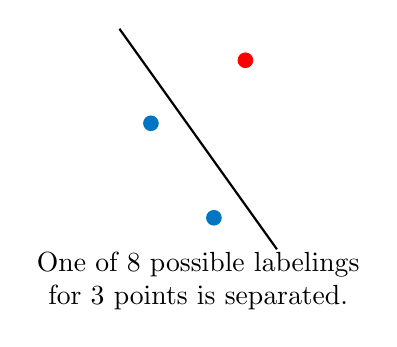
\begin{tikzpicture}[scale=0.8]
			\node[circle, fill=tudelftblue, inner sep=2pt] at (0,1) {};
			\node[circle, fill=red, inner sep=2pt] at (1.5,2) {};
			\node[circle, fill=tudelftblue, inner sep=2pt] at (1,-0.5) {};
			\draw[thick] (-0.5, 2.5) -- (2, -1);
			\node[align=center] at (0.75, -1.5) {One of 8 possible labelings\\for 3 points is separated.};
		\end{tikzpicture}
		\caption{A set of 3 points can be shattered by a line.}
	\end{subfigure}
	\hfill
	\begin{subfigure}{0.48\textwidth}
		\centering
		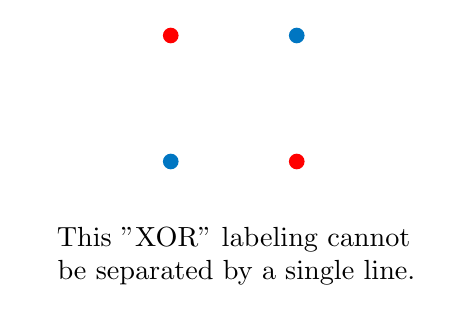
\begin{tikzpicture}[scale=0.8]
			\node[circle, fill=tudelftblue, inner sep=2pt] at (0,0) {};
			\node[circle, fill=tudelftblue, inner sep=2pt] at (2,2) {};
			\node[circle, fill=red, inner sep=2pt] at (0,2) {};
			\node[circle, fill=red, inner sep=2pt] at (2,0) {};
			\node[align=center, text width=5cm] at (1, -1.5) {This "XOR" labeling cannot be separated by a single line.};
		\end{tikzpicture}
		\caption{A set of 4 points cannot be shattered by a line.}
	\end{subfigure}
	\caption{Illustrating the VC-Dimension of a 2D linear classifier, which is 3.}
	\label{fig:vc_dimension}
\end{figure}

\paragraph{Theoretical Importance}
The main value of the VC-dimension is theoretical. It provides a probabilistic upper bound on the true error of a classifier based on its training error and its complexity $h$.  Conceptually, the bound is:
\[ \epsilon \le \epsilon_A + \text{ComplexityPenalty}(h, N, \eta) \]
This confirms our intuition: to keep the generalization error $\epsilon$ close to the training error $\epsilon_A$, we need a classifier with a small VC-dimension $h$.  In practice, these bounds are often too loose to be useful for direct calculation, but they provide the theoretical foundation for why controlling complexity is essential.

\subsection{Controlling Complexity with Support Vector Classifiers}
The \textbf{Support Vector Classifier (SVC)}, or \textbf{Support Vector Machine (SVM)}, is a linear classifier that is explicitly designed to control its complexity and thus generalize well. Instead of finding just \textit{any} hyperplane that separates the data (like the Perceptron), the SVM finds the single, unique, optimal hyperplane that has the \textbf{maximum margin} of separation between the two classes.

\paragraph{The Maximum Margin Principle}
The \textbf{margin} is the distance between the decision boundary and the closest data points from either class. These closest points, which lie on the edge of the margin, are called the \textbf{support vectors}. The intuition is that a larger margin corresponds to a more confident and robust classifier that is less sensitive to small variations in the training data.

Theoretically, maximizing the margin is equivalent to minimizing the classifier's VC-dimension. By finding the simplest possible boundary (in the maximum margin sense), the SVM aims to minimize the gap between the training error and the generalization error.


\paragraph{The Optimization Problem}
Maximizing the margin can be shown to be equivalent to minimizing the squared norm of the weight vector, $||\mathbf{w}||^2$. This leads to a constrained optimization problem, known as the \textbf{hard-margin SVM} formulation (for linearly separable data):
\begin{align}
	\min_{\mathbf{w}, b} \quad & \frac{1}{2} ||\mathbf{w}||^2                                                \\
	\text{subject to} \quad    & y_i(\mathbf{w}^T\mathbf{x}_i + b) \ge 1 \quad \text{for all } i=1, \dots, N
\end{align}
The constraints ensure that all data points are correctly classified and lie outside the margin. The solution to this problem is a decision boundary that depends only on the support vectors, making the model robust and memory-efficient.

\subsection{Non-Linear SVMs: The Kernel Trick}
The true power of Support Vector Machines is their ability to handle non-linearly separable data. This is achieved by combining the idea of feature maps with a clever mathematical shortcut known as the \textbf{Kernel Trick}.

The strategy is as follows:
\begin{enumerate}
	\item Project the original data from its low-dimensional feature space into a much higher-dimensional feature space using a non-linear mapping, $\phi(\mathbf{x})$.
	\item In this higher-dimensional space, the data may now be linearly separable.
	\item Find the maximum-margin linear classifier in this new feature space.
\end{enumerate}
The problem with this approach is that the new feature space can be enormous or even infinite-dimensional, making the computations intractable. This is where the Kernel Trick comes in.

The SVM's optimization problem and its final decision function only ever depend on the inner product (dot product) of feature vectors, not the vectors themselves. The \textbf{Kernel Trick} is to use a \textbf{kernel function}, $K(\mathbf{x}_i, \mathbf{x}_j)$, that computes the inner product of the data points in the high-dimensional space, $\phi(\mathbf{x}_i)^T \phi(\mathbf{x}_j)$, directly from the original low-dimensional vectors.
\begin{equation}
	K(\mathbf{x}_i, \mathbf{x}_j) = \phi(\mathbf{x}_i)^T \phi(\mathbf{x}_j)
\end{equation}
This allows us to get the full benefit of working in a high-dimensional space without ever having to explicitly perform the transformation, which is incredibly efficient.

\paragraph{Popular Kernel Functions}
By simply swapping the standard inner product $ \mathbf{x}_i^T \mathbf{x}_j $ with a kernel function, we can create powerful non-linear SVMs. Two popular kernels are:
\begin{itemize}
	\item \textbf{Polynomial Kernel:} Creates a polynomial decision boundary. The degree of the polynomial, $d$, is a hyperparameter.
	      \begin{equation}
		      K(\mathbf{x}_i, \mathbf{x}_j) = (\mathbf{x}_i^T \mathbf{x}_j + c)^d
	      \end{equation}
	\item \textbf{Radial Basis Function (RBF) Kernel:} A very powerful and popular general-purpose kernel. It can create complex, localized decision boundaries. Its hyperparameter, $\gamma$ (gamma), controls the flexibility of the boundary.
	      \begin{equation}
		      K(\mathbf{x}_i, \mathbf{x}_j) = \exp(-\gamma ||\mathbf{x}_i - \mathbf{x}_j||^2)
	      \end{equation}
\end{itemize}

\subsubsection{Chapter Conclusion}
Understanding \textbf{model complexity} is key to navigating the fundamental \textbf{Bias-Variance Tradeoff}. We saw that complexity is more than just the number of parameters and can be formally characterized by the \textbf{VC-Dimension}. This led us to the \textbf{Support Vector Machine}, a classifier explicitly designed to control complexity by finding a \textbf{maximum margin} solution. Finally, the \textbf{Kernel Trick} allows SVMs to efficiently learn complex, non-linear boundaries, making them one of the most powerful and theoretically elegant classifiers in machine learning.

\section{Regularisation}
\label{sec:ml_regularisation}

This final chapter focuses on \textbf{Regularisation}, a collection of essential techniques designed to combat overfitting. The core idea is to intentionally introduce a preference for simpler models during training, even if it means not fitting the training data as perfectly. As defined by Goodfellow et al., regularization encompasses any technique used to reduce a model's test error, possibly at the expense of an increased training error.

\subsection{The Problem of Overfitting}
As we've seen, a model with high complexity (or "capacity") can easily overfit a limited dataset. It learns not only the underlying signal but also the random noise specific to the training samples. A classic example is polynomial regression: a high-degree polynomial can perfectly pass through every training point but will likely oscillate wildly and perform poorly on new data. Regularisation aims to find a "sweet spot," like the quadratic fit below, that captures the general trend without memorizing the noise.


\subsection{The Regularisation Framework}
The most common way to implement regularisation is by adding a \textbf{penalty term}, $\Omega(\theta)$, to the standard loss function, $J(\theta)$. This creates a new, regularised loss function, $\tilde{J}(\theta)$:
\begin{equation}
	\tilde{J}(\theta) = J(\theta; X, y) + \alpha \Omega(\theta)
	\label{eq:regularisation_framework}
\end{equation}
The components of this framework are:
\begin{itemize}
	\item \textbf{$J(\theta; X, y)$:} The original \textbf{loss term} that measures how well the model with parameters $\theta$ fits the data (e.g., MSE or cross-entropy).
	\item \textbf{$\Omega(\theta)$:} The \textbf{regularisation penalty}. This term measures the complexity of the model. Common choices include penalizing the size of the model's weights.
	\item \textbf{$\alpha$:} The \textbf{regularisation parameter} ($\alpha \ge 0$). This is a hyperparameter that controls the strength of the penalty. It determines the tradeoff between fitting the training data well and keeping the model simple. A larger $\alpha$ encourages a simpler model.
\end{itemize}
During training, the optimizer now minimizes this combined objective. It is forced to find a set of parameters $\theta$ that not only achieves a low data-fitting error but also has low complexity.

\subsection{Parameter Norm Penalties}
This is the most common regularization strategy. It involves adding a penalty term $\Omega(\mathbf{w})$ to the loss function that is a function of the model's weights.

\subsubsection{L2 Regularisation (Weight Decay / Ridge)}
\textbf{L2 Regularisation} adds a penalty proportional to the squared L2 norm of the weight vector, $||\mathbf{w}||_2^2 = \sum_i w_i^2$. This is also known as \textbf{Ridge Regression} in the context of linear models.

The regularised loss function is:
\begin{equation}
	\tilde{J}(\mathbf{w}) = J(\mathbf{w}) + \frac{\alpha}{2} ||\mathbf{w}||_2^2
\end{equation}
This penalty discourages large weight values. During gradient descent, it results in an update rule that effectively shrinks the weights toward zero at each step, which is why it's often called \textbf{weight decay}. It encourages the model to use all features a little bit, rather than relying heavily on just a few.

\subsubsection{L1 Regularisation (Lasso)}
\textbf{L1 Regularisation} adds a penalty proportional to the L1 norm of the weight vector, $||\mathbf{w}||_1 = \sum_i |w_i|$. This is also known as \textbf{Lasso} (Least Absolute Shrinkage and Selection Operator) in linear models.

The regularised loss function is:
\begin{equation}
	\tilde{J}(\mathbf{w}) = J(\mathbf{w}) + \alpha ||\mathbf{w}||_1
\end{equation}
The L1 penalty has a unique and powerful property: it promotes \textbf{sparsity}. As the regularization strength $\alpha$ is increased, many of the model's weights are driven to be exactly zero. This means L1 regularization can be used for \textbf{automatic feature selection}, as it effectively removes irrelevant features from the model, leading to simpler and more interpretable results.

% === CHAPTER 2: Deep Learning ===
\chapter{Deep Learning}
\label{chap:dl}

\section{Feedforward Neural Networks}
\label{sec:dl_feedforward}

In the previous chapter, we explored classical machine learning algorithms where success hinged on the quality of the features provided to the model. A linear classifier on raw pixel values will fail, but given well-engineered features (e.g., histograms of gradients), it can excel. This process of \textbf{feature engineering} is laborious, domain-specific, and represents the core bottleneck in classical machine learning.

\textbf{Deep Learning} offers a radical alternative: instead of handcrafting features, we learn them directly from raw data. Deep feedforward networks, also known as \textbf{Multi-Layer Perceptrons (MLPs)}, achieve this by composing multiple layers of simple, parameterized transformations. Each layer learns a progressively more abstract representation of the input, culminating in a final layer that performs the task (e.g., classification). The network's parameters are adjusted end-to-end to minimize a loss function, simultaneously learning the feature extractor and the classifier.

More formally, the goal of a feedforward network is to approximate some target function $f^*$. For a classifier, this might be $y = f^*(\mathbf{x})$, which maps an input $\mathbf{x}$ to a category $y$. A feedforward network defines a parameterized mapping $\mathbf{y} = f(\mathbf{x}; \boldsymbol{\theta})$ and learns the parameters $\boldsymbol{\theta}$ that result in the best function approximation. These models are called \textit{feedforward} because information flows in one direction, which is from input $\mathbf{x}$, through intermediate computations, to output $\mathbf{y}$, without any feedback loops.

\subsection{Network Architecture and Notation}
A feedforward network is constructed by composing together many simpler functions, forming a \textbf{computational graph}. Consider a network represented as a chain of three functions:
\begin{equation}
	f(\mathbf{x}) = f^{(3)}(f^{(2)}(f^{(1)}(\mathbf{x})))
\end{equation}
The terminology for this architecture is as follows:
\begin{itemize}
	\item $f^{(1)}$ is the \textbf{first layer}, the one closest to the input.
	\item $f^{(2)}$ is a \textbf{hidden layer}. Its outputs are not directly observed in the training data; they are internal representations learned by the network.
	\item $f^{(3)}$ is the \textbf{output layer}, producing the final prediction.
	\item The number of layers in the chain is the \textbf{depth} of the network. This network has a depth of 3. The term ``deep learning'' refers to training networks with many such layers.
	\item The number of units (neurons) in a layer is its \textbf{width}.
\end{itemize}

\begin{figure}[H]
\centering
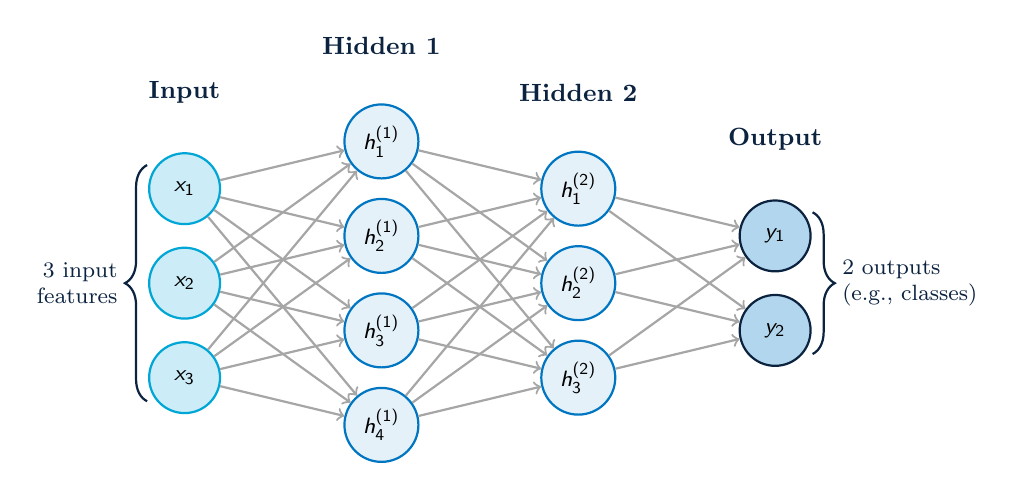
\begin{tikzpicture}[
    node distance=1.8cm and 2.5cm,
    neuron/.style={circle, draw=tudelftblue, fill=tudelftblue!10, thick, minimum size=0.9cm, font=\footnotesize},
    input neuron/.style={neuron, fill=tudelftcyan!20, draw=tudelftcyan},
    output neuron/.style={neuron, fill=tudelftblue!30, draw=tudelftdarkblue},
    connection/.style={->, thick, gray!70},
    layer label/.style={font=\small\bfseries, text=tudelftdarkblue}
]
    % Input Layer
    \node[input neuron] (x1) at (0, 1.2) {$x_1$};
    \node[input neuron] (x2) at (0, 0) {$x_2$};
    \node[input neuron] (x3) at (0, -1.2) {$x_3$};
    \node[layer label, above=0.5cm of x1] {Input};
    
    % Hidden Layer 1
    \node[neuron] (h11) at (2.5, 1.8) {$h_1^{(1)}$};
    \node[neuron] (h12) at (2.5, 0.6) {$h_2^{(1)}$};
    \node[neuron] (h13) at (2.5, -0.6) {$h_3^{(1)}$};
    \node[neuron] (h14) at (2.5, -1.8) {$h_4^{(1)}$};
    \node[layer label, above=0.5cm of h11] {Hidden 1};
    
    % Hidden Layer 2 (centered at y=0)
    \node[neuron] (h21) at (5, 1.2) {$h_1^{(2)}$};
    \node[neuron] (h22) at (5, 0) {$h_2^{(2)}$};
    \node[neuron] (h23) at (5, -1.2) {$h_3^{(2)}$};
    \node[layer label, above=0.5cm of h21] {Hidden 2};
    
    % Output Layer (centered at y=0)
    \node[output neuron] (y1) at (7.5, 0.6) {$y_1$};
    \node[output neuron] (y2) at (7.5, -0.6) {$y_2$};
    \node[layer label, above=0.5cm of y1] {Output};
    
    % Connections: Input -> Hidden 1
    \foreach \i in {1,2,3} {
        \foreach \j in {1,2,3,4} {
            \draw[connection] (x\i) -- (h1\j);
        }
    }
    
    % Connections: Hidden 1 -> Hidden 2
    \foreach \i in {1,2,3,4} {
        \foreach \j in {1,2,3} {
            \draw[connection] (h1\i) -- (h2\j);
        }
    }
    
    % Connections: Hidden 2 -> Output
    \foreach \i in {1,2,3} {
        \foreach \j in {1,2} {
            \draw[connection] (h2\i) -- (y\j);
        }
    }
    
    % Annotations
    \draw [decorate, decoration={brace, amplitude=8pt, raise=5pt}, thick, tudelftdarkblue] (7.8, 0.9) -- (7.8, -0.9) node [midway, right, xshift=12pt, align=left, font=\footnotesize] {2 outputs\\(e.g., classes)};
    \draw [decorate, decoration={brace, amplitude=8pt, raise=5pt, mirror}, thick, tudelftdarkblue] (-0.3, 1.5) -- (-0.3, -1.5) node [midway, left, xshift=-12pt, align=right, font=\footnotesize] {3 input\\features};
\end{tikzpicture}
\caption{Architecture of a feedforward neural network with two hidden layers. Arrows represent weighted connections. Each unit in a hidden layer computes a weighted sum of its inputs, adds a bias, and applies a non-linear activation function. This network has depth 4 (input + 2 hidden + output) and varying widths per layer.}
\label{fig:mlp_architecture}
\end{figure}

\subsubsection{The Computation Within a Layer}
Each layer $l$ performs a simple computation. Let $\mathbf{h}^{(l-1)}$ be the output of the previous layer (or the input $\mathbf{x}$ for the first layer). The layer computes:
\begin{equation}
	\mathbf{h}^{(l)} = g\left( \mathbf{W}^{(l)} \mathbf{h}^{(l-1)} + \mathbf{b}^{(l)} \right)
\end{equation}
where $\mathbf{W}^{(l)}$ is the \textbf{weight matrix}, $\mathbf{b}^{(l)}$ is the \textbf{bias vector}, and $g(\cdot)$ is a non-linear \textbf{activation function} applied element-wise. The weights and biases constitute the learnable parameters $\boldsymbol{\theta}$.

\subsubsection{Parameter Counting}
Understanding the number of parameters in a network is crucial for estimating its capacity and computational cost. Consider a simple network with:
\begin{itemize}
	\item Input dimensionality: $d_{in} = 2$
	\item One hidden layer with $d_h = 2$ neurons
	\item Output dimensionality: $d_{out} = 1$
\end{itemize}
The total number of parameters is calculated layer by layer:
\begin{enumerate}
	\item \textbf{Input to Hidden:} Weight matrix $\mathbf{W}^{(1)} \in \mathbb{R}^{d_h \times d_{in}} = \mathbb{R}^{2 \times 2}$ has $2 \times 2 = 4$ weights. Bias vector $\mathbf{b}^{(1)} \in \mathbb{R}^{d_h}$ has 2 biases. \textbf{Total: 6 parameters.}
	\item \textbf{Hidden to Output:} Weight matrix $\mathbf{W}^{(2)} \in \mathbb{R}^{d_{out} \times d_h} = \mathbb{R}^{1 \times 2}$ has $1 \times 2 = 2$ weights. Bias $b^{(2)} \in \mathbb{R}$ has 1 bias. \textbf{Total: 3 parameters.}
\end{enumerate}
\textbf{Grand Total:} $6 + 3 = 9$ parameters. Formally, the full model can be written as:
\begin{equation}
	f(\mathbf{x}; \boldsymbol{\theta}) = \mathbf{W}^{(2)} g\left( \mathbf{W}^{(1)} \mathbf{x} + \mathbf{b}^{(1)} \right) + b^{(2)}
\end{equation}
The goal of training is to find the values of $\boldsymbol{\theta} = \{\mathbf{W}^{(1)}, \mathbf{b}^{(1)}, \mathbf{W}^{(2)}, b^{(2)}\}$ such that $f(\mathbf{x}; \boldsymbol{\theta})$ approximates the target function $f^*(\mathbf{x})$.

\subsection{Activation Functions}
The non-linear activation function $g(\cdot)$ is the key ingredient that gives neural networks their power. Without it, a multi-layer network would collapse into a single linear transformation, regardless of its depth. This section details the most common activation functions.

\begin{figure}[H]
\begin{pycode}
z = np.linspace(-4, 4, 200)

# Activation Functions
relu = np.maximum(0, z)
leaky_relu = np.where(z > 0, z, 0.1 * z)
sigmoid = 1 / (1 + np.exp(-z))
tanh = np.tanh(z)

fig, axes = plt.subplots(1, 2, figsize=(12, 4.5))

# === Left: Activation Functions ===
axes[0].plot(z, relu, label=r'ReLU: $\max(0, z)$', color=utils.COLORS['primary'], linewidth=2.5)
axes[0].plot(z, leaky_relu, label=r'Leaky ReLU: $\max(0.1z, z)$', color=utils.COLORS['cyan'], linewidth=2, linestyle='--')
axes[0].plot(z, sigmoid, label=r'Sigmoid: $\sigma(z)$', color=utils.COLORS['red'], linewidth=2)
axes[0].plot(z, tanh, label='Tanh', color=utils.COLORS['green'], linewidth=2)

axes[0].axhline(0, color='gray', linewidth=0.5)
axes[0].axvline(0, color='gray', linewidth=0.5)
axes[0].set_title('Common Activation Functions')
axes[0].set_xlabel('$z$ (pre-activation)')
axes[0].set_ylabel('$g(z)$')
axes[0].legend(loc='upper left')
axes[0].set_ylim(-1.5, 4)
axes[0].grid(True, linestyle=':', alpha=0.5)

# === Right: Derivatives ===
# Derivatives
d_relu = np.where(z > 0, 1, 0).astype(float)
d_leaky_relu = np.where(z > 0, 1, 0.1)
d_sigmoid = sigmoid * (1 - sigmoid)
d_tanh = 1 - tanh**2

axes[1].plot(z, d_relu, label="ReLU'", color=utils.COLORS['primary'], linewidth=2.5)
axes[1].plot(z, d_leaky_relu, label="Leaky ReLU'", color=utils.COLORS['cyan'], linewidth=2, linestyle='--')
axes[1].plot(z, d_sigmoid, label="Sigmoid'", color=utils.COLORS['red'], linewidth=2)
axes[1].plot(z, d_tanh, label="Tanh'", color=utils.COLORS['green'], linewidth=2)

axes[1].axhline(0, color='gray', linewidth=0.5)
axes[1].axvline(0, color='gray', linewidth=0.5)
axes[1].set_title('Derivatives (Crucial for Backpropagation)')
axes[1].set_xlabel('$z$ (pre-activation)')
axes[1].set_ylabel("$g'(z)$")
axes[1].legend(loc='upper right')
axes[1].set_ylim(-0.1, 1.5)
axes[1].grid(True, linestyle=':', alpha=0.5)

utils.save_and_include("activation_functions.pdf", width=r"1.0\textwidth")
\end{pycode}
\caption{\textbf{Left:} Common activation functions. ReLU is the modern default due to its simplicity and favorable gradient properties. \textbf{Right:} The derivatives of these functions. Note how Sigmoid and Tanh derivatives saturate to near-zero for large $|z|$, which can cause vanishing gradients. ReLU's derivative is a constant 1 for positive inputs, ensuring healthy gradient flow.}
\label{fig:activation_functions}
\end{figure}

\paragraph{ReLU (Rectified Linear Unit):} Defined as $g(z) = \max\{0, z\}$. This is the default choice for modern deep learning for several reasons:
\begin{itemize}
    \item \textbf{Computational Efficiency:} It involves only a simple thresholding operation.
    \item \textbf{Sparsity:} For negative inputs, the output is exactly zero, leading to sparse activations which can improve efficiency and representation.
    \item \textbf{Non-saturating Gradient:} For positive inputs, the gradient is 1, which mitigates the \textit{vanishing gradient problem} that plagued earlier networks using Sigmoid or Tanh.
\end{itemize}
A known issue is the \textbf{Dying ReLU Problem}: if a neuron's input is always negative, its gradient is always zero, and it stops learning entirely.

\paragraph{Leaky ReLU:} A variant designed to fix the dying ReLU problem: $g(z) = \max\{\alpha z, z\}$, where $\alpha$ is a small constant (e.g., 0.01 or 0.1). This provides a small, non-zero gradient when the unit is not active.

\paragraph{Sigmoid:} Defined as $\sigma(z) = \frac{1}{1+e^{-z}}$. It squashes the input to the range $(0, 1)$. Historically important, it is now mostly used in output layers for binary classification (to produce a probability) rather than in hidden layers, due to its tendency to saturate.

\paragraph{Tanh (Hyperbolic Tangent):} Defined as $\tanh(z) = \frac{e^z - e^{-z}}{e^z + e^{-z}}$. Similar to Sigmoid but outputs are centered around zero, in the range $(-1, 1)$. This can be beneficial as it means the output of one layer has zero mean, which can help with the dynamics of training in some cases.

\subsection{The Need for Non-Linearity: The XOR Problem}
Why is non-linearity so essential? A linear model defines a hyperplane decision boundary: $y = \mathbf{w}^T \mathbf{x} + b$. Consider the classic \textbf{XOR (exclusive or)} problem:
\begin{itemize}
	\item Inputs: $\mathbf{X} = \{[0, 0]^T, [0, 1]^T, [1, 0]^T, [1, 1]^T\}$
	\item Labels: $Y = \{0, 1, 1, 0\}$
\end{itemize}
These points are \textbf{not linearly separable}. No single straight line can separate the class-0 points $\{(0,0), (1,1)\}$ from the class-1 points $\{(0,1), (1,0)\}$.

\begin{figure}[H]
\centering
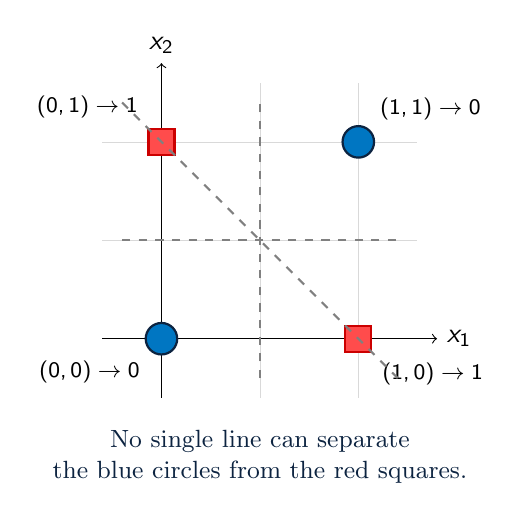
\begin{tikzpicture}[scale=2.5]
    % Grid
    \draw[gray!30, very thin] (-0.3, -0.3) grid[step=0.5] (1.3, 1.3);
    \draw[->] (-0.3, 0) -- (1.4, 0) node[right] {$x_1$};
    \draw[->] (0, -0.3) -- (0, 1.4) node[above] {$x_2$};
    
    % Points - Class 0 (Blue circles)
    \node[circle, fill=tudelftblue, draw=tudelftdarkblue, thick, minimum size=0.4cm, label={[font=\footnotesize]below left:$(0,0) \to 0$}] at (0, 0) {};
    \node[circle, fill=tudelftblue, draw=tudelftdarkblue, thick, minimum size=0.4cm, label={[font=\footnotesize]above right:$(1,1) \to 0$}] at (1, 1) {};
    
    % Points - Class 1 (Red squares)
    \node[regular polygon, regular polygon sides=4, fill=red!70, draw=red!80!black, thick, minimum size=0.4cm, label={[font=\footnotesize]above left:$(0,1) \to 1$}] at (0, 1) {};
    \node[regular polygon, regular polygon sides=4, fill=red!70, draw=red!80!black, thick, minimum size=0.4cm, label={[font=\footnotesize]below right:$(1,0) \to 1$}] at (1, 0) {};
    
    % Failed linear boundaries (dashed, to show impossibility)
    \draw[dashed, thick, gray] (-0.2, 0.5) -- (1.2, 0.5);
    \draw[dashed, thick, gray] (0.5, -0.2) -- (0.5, 1.2);
    \draw[dashed, thick, gray] (-0.2, 1.2) -- (1.2, -0.2);
    
    % Annotation
    \node[align=center, font=\small, text=tudelftdarkblue] at (0.5, -0.6) {No single line can separate\\the blue circles from the red squares.};
\end{tikzpicture}
\caption{The XOR problem is not linearly separable. The dashed lines show examples of linear decision boundaries, none of which can correctly classify all four points. This demonstrates the fundamental limitation of linear models.}
\label{fig:xor_problem}
\end{figure}

\subsubsection{The Solution: Learned Representations}
The key insight of deep learning is that we can use a hidden layer to \textbf{transform} the input into a new representation where the problem \textit{becomes} linearly separable. We introduce a hidden layer $\mathbf{h} = g(\mathbf{W}^{(1)} \mathbf{x} + \mathbf{b}^{(1)})$ with a non-linear activation $g$. The output is then a linear function of this hidden representation: $y = \mathbf{w}^T \mathbf{h} + b$.

The full model is:
\begin{equation}
	f(\mathbf{x}) = \mathbf{w}^T g(\mathbf{W}^{(1)} \mathbf{x} + \mathbf{b}^{(1)}) + b
\end{equation}
By learning the parameters $\mathbf{W}^{(1)}, \mathbf{b}^{(1)}$, the network learns a \textit{feature map} $\phi(\mathbf{x}) = g(\mathbf{W}^{(1)} \mathbf{x} + \mathbf{b}^{(1)})$ that ``unfolds'' the data so that a simple linear classifier on $\mathbf{h}$ can solve the original problem. This is the essence of \textbf{representation learning}.

\subsection{Worked Example: Solving XOR}
Let's construct a network that solves XOR using the ReLU activation function $g(z) = \max\{0, z\}$.

\textbf{Architecture:} 2 input units $\to$ 2 hidden units $\to$ 1 output unit.

\textbf{Manually Designed Parameters:}
\begin{equation}
	\mathbf{W}^{(1)} = \begin{pmatrix} 1 & 1 \\ 1 & 1 \end{pmatrix}, \quad
	\mathbf{b}^{(1)} = \begin{pmatrix} 0 \\ -1 \end{pmatrix}, \quad
	\mathbf{w} = \begin{pmatrix} 1 \\ -2 \end{pmatrix}, \quad
	b = 0
\end{equation}

\textbf{Forward Pass Computation:}
We compute $\mathbf{h} = \max\{0, \mathbf{W}^{(1)} \mathbf{x} + \mathbf{b}^{(1)}\}$ and then $y = \mathbf{w}^T \mathbf{h} + b$ for each input.

\begin{table}[H]
\centering
\begin{tblr}{
  colspec = {c|c|c|c|c},
  row{1} = {font=\bfseries},
  hline{1,2,Z} = {solid},
}
Input $\mathbf{x}$ & $\mathbf{W}^{(1)}\mathbf{x} + \mathbf{b}^{(1)}$ & $\mathbf{h} = \text{ReLU}(\cdot)$ & $y = \mathbf{w}^T\mathbf{h}$ & Target \\
$[0, 0]^T$ & $[0, -1]^T$ & $[0, 0]^T$ & $1(0) - 2(0) = \mathbf{0}$ & 0 \\
$[0, 1]^T$ & $[1, 0]^T$ & $[1, 0]^T$ & $1(1) - 2(0) = \mathbf{1}$ & 1 \\
$[1, 0]^T$ & $[1, 0]^T$ & $[1, 0]^T$ & $1(1) - 2(0) = \mathbf{1}$ & 1 \\
$[1, 1]^T$ & $[2, 1]^T$ & $[2, 1]^T$ & $1(2) - 2(1) = \mathbf{0}$ & 0 \\
\end{tblr}
\caption{Step-by-step computation of the XOR network, showing the hidden representation $\mathbf{h}$ and the final output $y$ for each input.}
\label{tab:xor_computation}
\end{table}

The network correctly computes the XOR function for all inputs. The key is looking at the hidden representation column: the hidden layer has mapped the four input points to only three distinct points in the hidden space. Crucially, the class-0 inputs $(0,0)$ and $(1,1)$ are now separated from the class-1 inputs.

\begin{figure}[H]
\begin{pycode}
# Define our XOR Network Parameters manually to match the worked example
W = np.array([[1, 1], [1, 1]])
c = np.array([0, -1])
w = np.array([1, -2])
b = 0

def relu(z):
    return np.maximum(0, z)

def forward(X):
    z = X @ W + c
    h = relu(z)
    y = h @ w + b
    return h, y

# Generate Grid for Input Space
resolution = 0.02
x_min, x_max = -0.3, 1.3
xx1, xx2 = np.meshgrid(np.arange(x_min, x_max, resolution),
                       np.arange(x_min, x_max, resolution))
X_grid = np.array([xx1.ravel(), xx2.ravel()]).T

# Forward pass on grid
H_grid, Y_grid = forward(X_grid)
Y_grid_reshaped = Y_grid.reshape(xx1.shape)

# XOR Data Points
X_xor = np.array([[0,0], [0,1], [1,0], [1,1]])
y_xor = np.array([0, 1, 1, 0])
colors = [utils.COLORS['primary'] if y == 0 else utils.COLORS['red'] for y in y_xor]
markers = ['o' if y==0 else 's' for y in y_xor]

# === Plotting ===
fig, axes = plt.subplots(1, 2, figsize=(11, 4.5))

# 1. Input Space Decision Boundary
axes[0].contourf(xx1, xx2, Y_grid_reshaped, alpha=0.5, levels=[-0.5, 0.5, 1.5],
                 colors=[utils.COLORS['light_bg'][0], utils.COLORS['light_bg'][2]])
# Draw the actual non-linear decision boundary (contour at y=0.5)
axes[0].contour(xx1, xx2, Y_grid_reshaped, levels=[0.5], colors=utils.COLORS['dark'], linewidths=2)

for i in range(4):
    axes[0].scatter(X_xor[i, 0], X_xor[i, 1], c=colors[i], marker=markers[i], s=150, edgecolors='k', linewidths=1.5, zorder=10)

axes[0].set_title('Input Space $(x_1, x_2)$\n(Non-linear Decision Boundary)', fontsize=11)
axes[0].set_xlabel('$x_1$')
axes[0].set_ylabel('$x_2$')
axes[0].set_xlim(-0.3, 1.3)
axes[0].set_ylim(-0.3, 1.3)
axes[0].set_aspect('equal')

# 2. Hidden Space Representation
H_xor, _ = forward(X_xor)

# Define h-space grid for background
h_min, h_max = -0.3, 2.3
hh1, hh2 = np.meshgrid(np.arange(h_min, h_max, resolution),
                       np.arange(h_min, h_max, resolution))
H_grid_manual = np.array([hh1.ravel(), hh2.ravel()]).T
Y_h_space = H_grid_manual @ w + b
Y_h_space = Y_h_space.reshape(hh1.shape)

axes[1].contourf(hh1, hh2, Y_h_space, alpha=0.5, levels=[-3, 0.5, 3],
                 colors=[utils.COLORS['light_bg'][0], utils.COLORS['light_bg'][2]])
# Linear decision boundary in hidden space: w^T h = 0.5 => h1 - 2*h2 = 0.5 => h2 = (h1 - 0.5)/2
axes[1].contour(hh1, hh2, Y_h_space, levels=[0.5], colors=utils.COLORS['dark'], linewidths=2)

# Plot hidden space points - handle collision at (1,0) where both (0,1) and (1,0) map
# Point 0: (0,0) -> (0,0) - blue circle (class 0)
axes[1].scatter(H_xor[0, 0], H_xor[0, 1], c=utils.COLORS['primary'], marker='o', s=150, edgecolors='k', linewidths=1.5, zorder=10)

# Points 1 and 2: (0,1) and (1,0) both -> (1,0) - plot ONE red square with double ring to show collision
axes[1].scatter(1, 0, c=utils.COLORS['red'], marker='s', s=200, edgecolors='k', linewidths=2.5, zorder=10)
axes[1].scatter(1, 0, c='none', marker='s', s=350, edgecolors=utils.COLORS['red'], linewidths=2, zorder=9)  # outer ring

# Point 3: (1,1) -> (2,1) - blue circle (class 0)
axes[1].scatter(H_xor[3, 0], H_xor[3, 1], c=utils.COLORS['primary'], marker='o', s=150, edgecolors='k', linewidths=1.5, zorder=10)

# Annotations for the hidden space points - with arrows for clarity
axes[1].annotate(r'$(0,0) \to (0,0)$', xy=(0, 0), xytext=(0.3, 0.5), fontsize=8, color=utils.COLORS['dark'],
                 arrowprops=dict(arrowstyle='->', color=utils.COLORS['dark'], lw=0.8))
axes[1].annotate(r'$(0,1), (1,0) \to (1,0)$', xy=(1, 0), xytext=(1.15, 0.5), fontsize=8, color=utils.COLORS['dark'],
                 arrowprops=dict(arrowstyle='->', color=utils.COLORS['dark'], lw=0.8))
axes[1].annotate(r'$(1,1) \to (2,1)$', xy=(2, 1), xytext=(1.6, 0.55), fontsize=8, color=utils.COLORS['dark'],
                 arrowprops=dict(arrowstyle='->', color=utils.COLORS['dark'], lw=0.8))


axes[1].set_title(r'Hidden Space $(h_1, h_2)$' + '\n(Linear Decision Boundary!)', fontsize=11)
axes[1].set_xlabel(r'$h_1 = \max(0, x_1+x_2)$')
axes[1].set_ylabel(r'$h_2 = \max(0, x_1+x_2-1)$')
axes[1].set_xlim(-0.3, 2.5)
axes[1].set_ylim(-0.3, 1.3)
axes[1].set_aspect('equal')

utils.save_and_include("xor_solution_enhanced.pdf", width=r"1.0\textwidth")
\end{pycode}
\caption{Solving XOR with a hidden layer. \textbf{Left:} The learned decision boundary in the original input space is non-linear (a composition of two lines due to ReLU). \textbf{Right:} In the hidden representation space $(h_1, h_2)$, the four original points are mapped to only three locations, and these are now linearly separable. The network has learned a representation that makes the problem easy.}
\label{fig:xor_solution}
\end{figure}

\subsection{Training Neural Networks with Gradient Descent}
How do we find the parameters $\boldsymbol{\theta}$ that minimize the loss? In the XOR example, we manually crafted a solution, but for real problems with millions of parameters, this is impossible. We rely on \textbf{Gradient Descent}.

The idea is simple: start with random parameters, compute the gradient of the loss function with respect to all parameters, and iteratively update the parameters in the direction that reduces the loss.
\begin{equation}
	\boldsymbol{\theta}' = \boldsymbol{\theta} - \epsilon \nabla_{\boldsymbol{\theta}} J(\boldsymbol{\theta})
\end{equation}
where $\epsilon$ is the \textbf{learning rate}, a crucial hyperparameter that controls the step size.

\paragraph{Stochastic Gradient Descent (SGD):}
Computing the gradient over the entire dataset (\textbf{Batch Gradient Descent}) is computationally prohibitive for large datasets. \textbf{Stochastic Gradient Descent (SGD)} instead computes an estimate of the gradient using a small random subset of the data called a \textbf{mini-batch}:
\begin{equation}
	\boldsymbol{\theta}' = \boldsymbol{\theta} - \epsilon \frac{1}{|\mathcal{B}|} \sum_{i \in \mathcal{B}} \nabla_{\boldsymbol{\theta}} L(\mathbf{x}^{(i)}, y^{(i)}; \boldsymbol{\theta})
\end{equation}
where $\mathcal{B}$ is the mini-batch. This introduces noise into the gradient estimate, but it allows for much faster updates and, surprisingly, the noise can even help escape shallow local minima.

\begin{figure}[H]
\begin{pycode}
# Visualize Gradient Descent on a 2D loss surface (Rosenbrock-like function for visual appeal)
from matplotlib.colors import LogNorm

# Define a loss surface (simple quadratic for clarity)
def loss_func(w1, w2):
    # An elongated valley loss landscape
    return 0.5 * (w1**2 + 10 * w2**2)

# Generate grid for contour plot
w1_range = np.linspace(-3, 3, 100)
w2_range = np.linspace(-1.5, 1.5, 100)
W1, W2 = np.meshgrid(w1_range, w2_range)
L = loss_func(W1, W2)

# Simulate Gradient Descent
def gd_update(w, lr, grad_func):
    g = grad_func(w)
    return w - lr * g

def grad_loss(w):
    return np.array([w[0], 10 * w[1]])

# Run GD
np.random.seed(42)
lr = 0.15
w_init = np.array([-2.5, 1.2])
trajectory = [w_init.copy()]
w = w_init.copy()
for _ in range(15):
    w = gd_update(w, lr, grad_loss)
    trajectory.append(w.copy())
trajectory = np.array(trajectory)

fig, ax = plt.subplots(figsize=(8, 5))

# Contour plot
contour = ax.contour(W1, W2, L, levels=15, cmap='Blues', linewidths=0.7)
ax.contourf(W1, W2, L, levels=15, cmap='Blues', alpha=0.3)
ax.clabel(contour, inline=True, fontsize=7, fmt='%.1f')

# Plot trajectory
ax.plot(trajectory[:, 0], trajectory[:, 1], 'o-', color=utils.COLORS['red'], markersize=6, linewidth=1.5, label='GD Path')
ax.scatter(trajectory[0, 0], trajectory[0, 1], s=100, c=utils.COLORS['red'], marker='X', zorder=10, edgecolors='k', label='Start')
ax.scatter(0, 0, s=150, c=utils.COLORS['green'], marker='*', zorder=10, edgecolors='k', label='Optimum')

ax.set_xlabel('$w_1$')
ax.set_ylabel('$w_2$')
ax.set_title('Gradient Descent on a Loss Surface')
ax.legend(loc='upper right')
ax.set_xlim(-3, 3)
ax.set_ylim(-1.5, 1.5)

utils.save_and_include("gradient_descent_contour.pdf", width=r"0.8\textwidth")
\end{pycode}
\caption{Gradient descent visualized on a 2D loss contour. The red path shows the trajectory of the parameters as they are iteratively updated in the direction of steepest descent. The algorithm converges towards the global minimum (green star). Notice how the trajectory can oscillate in directions of high curvature (steep gradients).}
\label{fig:gd_contour}
\end{figure}

\subsection{The Universal Approximation Theorem}
A natural question arises: what functions can a neural network represent? The \textbf{Universal Approximation Theorem} provides a powerful theoretical answer.

\begin{tcolorbox}[colback=tudelftblue!5!white, colframe=tudelftblue, title=Universal Approximation Theorem]
A feedforward network with a single hidden layer containing a finite number of neurons can approximate any continuous function on a compact subset of $\mathbb{R}^n$ to arbitrary accuracy, provided the activation function is non-polynomial (e.g., Sigmoid, Tanh, or ReLU).
\end{tcolorbox}

This is a remarkable result: it tells us that neural networks are \textbf{universal function approximators}. However, the theorem comes with crucial caveats:
\begin{itemize}
	\item \textbf{Existence, not construction:} It guarantees that a solution \textit{exists} but says nothing about how to find it (i.e., whether gradient descent will converge to it).
	\item \textbf{Width, not depth:} It proves that a single, sufficiently \textit{wide} layer is enough. It does not explain the empirical success of \textit{deep} (many-layered) networks. In practice, depth is often more parameter-efficient than width for approximating complex functions.
	\item \textbf{No guarantees on size:} The number of neurons required could be astronomically large for complex functions.
\end{itemize}
In essence, the theorem assures us that neural networks are a flexible enough model family. The practical challenge lies in finding a good solution within the vast parameter space, which is the domain of optimization algorithms and the art of deep learning.

\subsection{Depth vs. Width: Why ``Deep'' Learning?}
If a single wide layer is theoretically sufficient, why do we use deep networks with many layers?

\paragraph{Hierarchical Representations:} Many real-world functions (like image recognition) have a hierarchical structure. Early layers can learn simple features (edges, colors), intermediate layers combine these into parts (eyes, noses), and later layers assemble parts into objects (faces). Depth allows the network to naturally capture this compositional structure.

\paragraph{Exponential Efficiency:} For certain classes of functions, deep networks can represent them with exponentially fewer parameters than a shallow network of the same accuracy. Intuitively, depth allows for efficient re-use of computations. A feature learned in an early layer can be combined in many different ways by later layers, leading to combinatorial richness.

\paragraph{Empirical Success:} In practice, deep networks consistently outperform shallow ones on complex tasks like image classification, natural language processing, and game playing, even when the total number of parameters is matched. The inductive bias towards hierarchical, compositional features seems to match the structure of many problems we care about.


\section{Loss Functions}
\label{sec:dl_loss}

In the previous section, we saw how to build feedforward networks and update their weights using gradient descent. But gradient descent requires a scalar objective function, which is a single number that tells us how ``wrong'' our model is. This section answers a fundamental question: \textbf{how do we define this objective?}

The choice of loss function is not arbitrary. A principled approach comes from the framework of \textbf{Maximum Likelihood Estimation (MLE)}, which connects our learning objective to the goal of finding a model that best explains the observed data.

\subsection{Maximum Likelihood Estimation}
Suppose we have a training set of $m$ samples $\mathcal{D} = \{\mathbf{x}^{(1)}, \mathbf{x}^{(2)}, \ldots, \mathbf{x}^{(m)}\}$, drawn independently and identically distributed (i.i.d.) from an unknown true data distribution $p_{\text{data}}(\mathbf{x})$. Our model defines a family of probability distributions $p_{\text{model}}(\mathbf{x}; \boldsymbol{\theta})$ parameterized by $\boldsymbol{\theta}$.

The \textbf{Maximum Likelihood Estimator} chooses the parameters that maximize the probability of the observed data under our model:
\begin{equation}
	\boldsymbol{\theta}_{\text{ML}} = \arg\max_{\boldsymbol{\theta}} p_{\text{model}}(\mathcal{D}; \boldsymbol{\theta})
\end{equation}
Thanks to the i.i.d. assumption, the probability of the entire dataset is the product of probabilities for each sample:
\begin{equation}
	\boldsymbol{\theta}_{\text{ML}} = \arg\max_{\boldsymbol{\theta}} \prod_{i=1}^{m} p_{\text{model}}(\mathbf{x}^{(i)}; \boldsymbol{\theta})
\end{equation}
Multiplying many probabilities (values between 0 and 1) quickly leads to numerical underflow. To solve this, we take the logarithm. Since $\log$ is a monotonically increasing function, it preserves the $\arg\max$. Products become sums:
\begin{equation}
	\boldsymbol{\theta}_{\text{ML}} = \arg\max_{\boldsymbol{\theta}} \sum_{i=1}^{m} \log p_{\text{model}}(\mathbf{x}^{(i)}; \boldsymbol{\theta})
\end{equation}
Dividing by $m$ (which does not change the $\arg\max$) gives us the expectation with respect to the empirical data distribution $\hat{p}_{\text{data}}$:
\begin{equation}
	\boldsymbol{\theta}_{\text{ML}} = \arg\max_{\boldsymbol{\theta}} \mathbb{E}_{\mathbf{x} \sim \hat{p}_{\text{data}}} \left[ \log p_{\text{model}}(\mathbf{x}; \boldsymbol{\theta}) \right]
\end{equation}
This is our training objective: maximize the average log-probability of the data under our model.

\subsection{KL Divergence and Cross-Entropy}
An alternative interpretation of MLE comes from information theory. We want our model distribution $p_{\text{model}}$ to be ``close'' to the true data distribution $p_{\text{data}}$. A natural measure of the dissimilarity between two distributions is the \textbf{Kullback-Leibler (KL) Divergence}:
\begin{equation}
	D_{\text{KL}}(p_{\text{data}} \| p_{\text{model}}) = \mathbb{E}_{\mathbf{x} \sim p_{\text{data}}} \left[ \log \frac{p_{\text{data}}(\mathbf{x})}{p_{\text{model}}(\mathbf{x}; \boldsymbol{\theta})} \right]
\end{equation}
Expanding the logarithm:
\begin{equation}
	D_{\text{KL}}(p_{\text{data}} \| p_{\text{model}}) = \mathbb{E}_{\mathbf{x} \sim p_{\text{data}}} [\log p_{\text{data}}(\mathbf{x})] - \mathbb{E}_{\mathbf{x} \sim p_{\text{data}}} [\log p_{\text{model}}(\mathbf{x}; \boldsymbol{\theta})]
\end{equation}
The first term, $-H(p_{\text{data}})$, is the negative entropy of the data distribution, which does not depend on $\boldsymbol{\theta}$. Therefore, minimizing the KL divergence is equivalent to minimizing the \textbf{negative log-likelihood}, which is known as the \textbf{Cross-Entropy}:
\begin{equation}
	H(p_{\text{data}}, p_{\text{model}}) = -\mathbb{E}_{\mathbf{x} \sim p_{\text{data}}} [\log p_{\text{model}}(\mathbf{x}; \boldsymbol{\theta})]
\end{equation}

\begin{tcolorbox}[colback=tudelftblue!5!white, colframe=tudelftblue, title=Equivalent Objectives]
The following are all equivalent objectives for training:
\begin{itemize}
	\item Maximize the \textbf{log-likelihood} (MLE)
	\item Minimize the \textbf{negative log-likelihood}
	\item Minimize the \textbf{KL divergence} from the data to the model
	\item Minimize the \textbf{cross-entropy} between data and model
\end{itemize}
\end{tcolorbox}

\subsection{Conditional Likelihood for Classification}
In most supervised learning problems, we are not interested in modeling the distribution of inputs $p(\mathbf{x})$. Instead, we want to predict labels $y$ given inputs $\mathbf{x}$. This leads us to the \textbf{conditional log-likelihood}:
\begin{equation}
	\boldsymbol{\theta}_{\text{ML}} = \arg\max_{\boldsymbol{\theta}} \sum_{i=1}^{m} \log p_{\text{model}}(y^{(i)} | \mathbf{x}^{(i)}; \boldsymbol{\theta})
\end{equation}
The form of $p_{\text{model}}(y | \mathbf{x})$ depends on the task:
\begin{itemize}
	\item For \textbf{binary classification}: $y \in \{0, 1\}$, modeled by a Bernoulli distribution.
	\item For \textbf{multiclass classification}: $y \in \{1, 2, \ldots, K\}$, modeled by a Categorical distribution.
	\item For \textbf{regression}: $y \in \mathbb{R}$, often modeled by a Gaussian (which leads to the familiar MSE loss).
\end{itemize}
The \textbf{output unit} of the network (e.g., Sigmoid, Softmax, Linear) determines which distribution we are using, and thus the specific form of the loss function.

\subsection{Binary Classification: Logistic Regression}
For binary classification, we need our model to output a probability $\hat{y} = P(y=1 | \mathbf{x}) \in [0, 1]$. A naïve approach is to use a linear output and clamp it: $\hat{y} = \max\{0, \min\{1, \mathbf{w}^T\mathbf{x} + b\}\}$. However, this kills gradients outside the $[0, 1]$ interval.

The solution is the \textbf{Sigmoid} (or logistic) function, which smoothly squashes any real number into $(0, 1)$:
\begin{equation}
	\sigma(z) = \frac{1}{1 + e^{-z}}
\end{equation}

\begin{figure}[H]
\centering
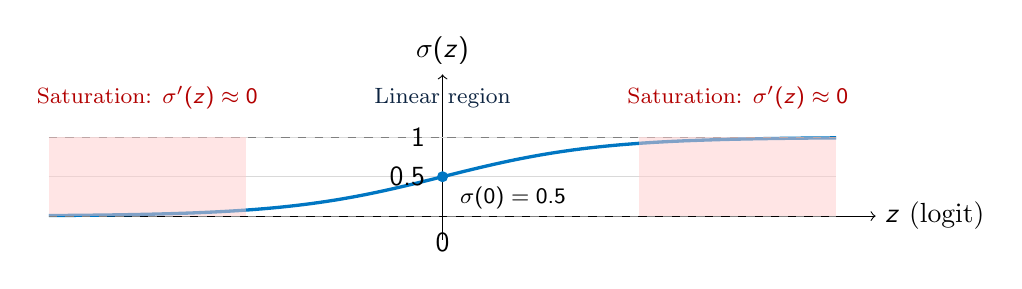
\begin{tikzpicture}[scale=1.0]
    % Axes
    \draw[->] (-5, 0) -- (5.5, 0) node[right] {$z$ (logit)};
    \draw[->] (0, -0.3) -- (0, 1.8) node[above] {$\sigma(z)$};
    
    % Grid lines
    \draw[gray!30, thin] (-5, 0.5) -- (5, 0.5);
    \draw[gray!30, thin] (-5, 1) -- (5, 1);
    
    % Sigmoid curve
    \draw[tudelftblue, very thick, domain=-5:5, samples=100] plot (\x, {1/(1+exp(-\x))});
    
    % Asymptotes
    \draw[dashed, gray] (-5, 1) -- (5, 1);
    \draw[dashed, gray] (-5, 0) -- (5, 0);
    
    % Labels for asymptotes
    \node[left] at (-0.1, 1) {$1$};
    \node[left] at (-0.1, 0.5) {$0.5$};
    \node[below] at (0, -0.1) {$0$};
    
    % Saturation regions
    \fill[red!20, opacity=0.5] (-5, 0) rectangle (-2.5, 1);
    \fill[red!20, opacity=0.5] (2.5, 0) rectangle (5, 1);
    
    % Annotations - positioned above the plot to avoid overlap
    \node[font=\footnotesize, text=red!70!black] at (-3.75, 1.5) {Saturation: $\sigma'(z) \approx 0$};
    \node[font=\footnotesize, text=red!70!black] at (3.75, 1.5) {Saturation: $\sigma'(z) \approx 0$};
    \node[font=\footnotesize, text=tudelftdarkblue] at (0, 1.5) {Linear region};
    
    % Key point
    \fill[tudelftblue] (0, 0.5) circle (2pt);
    \node[below right, font=\footnotesize] at (0.1, 0.5) {$\sigma(0) = 0.5$};
\end{tikzpicture}
\caption{The Sigmoid function. It maps any real-valued logit $z$ to a probability in $(0, 1)$. In the \textbf{saturation regions} (red), the gradient $\sigma'(z) = \sigma(z)(1-\sigma(z))$ is very small, which can cause slow learning if the wrong loss function is used.}
\label{fig:sigmoid_annotated}
\end{figure}

The input $z = \mathbf{w}^T\mathbf{x} + b$ is called the \textbf{logit}. The complete model for \textbf{logistic regression} is:
\begin{equation}
	\hat{y} = \sigma(\mathbf{w}^T\mathbf{x} + b)
\end{equation}

\subsubsection{The Binary Cross-Entropy Loss}
Since $y \in \{0, 1\}$ follows a Bernoulli distribution, the likelihood is $P(y | \mathbf{x}) = \hat{y}^y (1-\hat{y})^{1-y}$. Taking the negative log gives the \textbf{Binary Cross-Entropy} (BCE) loss:
\begin{equation}
	L_{\text{BCE}}(\hat{y}, y) = -y \log \hat{y} - (1-y) \log(1 - \hat{y})
\end{equation}
This can be understood intuitively:
\begin{itemize}
	\item If the true label is $y=1$: The loss is $-\log \hat{y}$. This penalizes low predictions heavily.
	\item If the true label is $y=0$: The loss is $-\log(1-\hat{y})$. This penalizes high predictions heavily.
\end{itemize}

\subsubsection{Why Not Squared Error?}
A natural question is: why not simply use the Squared Error $L_{\text{SE}} = \frac{1}{2}(\hat{y} - y)^2$? The answer lies in the gradients.

When we compute the gradient of the loss with respect to the logit $z$:
\begin{itemize}
	\item \textbf{Squared Error:} $\frac{\partial L_{\text{SE}}}{\partial z} = (\hat{y} - y) \cdot \sigma'(z) = (\hat{y} - y) \cdot \hat{y}(1-\hat{y})$
	\item \textbf{Cross-Entropy:} $\frac{\partial L_{\text{BCE}}}{\partial z} = \hat{y} - y$
\end{itemize}
With Squared Error, the gradient includes the term $\hat{y}(1-\hat{y})$. When the model is \textit{confidently wrong} (e.g., $y=1$ but $\hat{y} \approx 0$), this term is nearly zero, causing the \textbf{vanishing gradient problem}. Cross-Entropy's gradient is simply proportional to the error $(\hat{y} - y)$, which remains large when predictions are wrong.

\begin{figure}[H]
\begin{pycode}
# Plot comparing gradients of SE vs CE for Sigmoid
z = np.linspace(-10, 10, 400)
y_pred = 1 / (1 + np.exp(-z))
t = 1 # Target is class 1

# Losses
loss_ce = -np.log(y_pred + 1e-10)  # add eps for stability
loss_se = 0.5 * (y_pred - t)**2

# Gradients w.r.t z
grad_ce = y_pred - t
grad_se = (y_pred - t) * y_pred * (1 - y_pred)

fig, axes = plt.subplots(1, 2, figsize=(12, 5))

# Plot Losses
axes[0].plot(z, loss_ce, label='Cross-Entropy', color=utils.COLORS['primary'], linewidth=2)
axes[0].plot(z, loss_se, label='Squared Error', color=utils.COLORS['red'], linewidth=2)
axes[0].set_title(r'Loss Value (Target $y=1$)')
axes[0].set_xlabel(r'$z$ (Logit)')
axes[0].set_ylabel('Loss')
axes[0].legend()
axes[0].set_ylim(0, 4)
axes[0].grid(True, linestyle=':', alpha=0.6)

# Plot Derivatives (Magnitude)
axes[1].plot(z, np.abs(grad_ce), label=r'$|\nabla_z L_{CE}| = |\hat{y}-y|$', color=utils.COLORS['primary'], linewidth=2)
axes[1].plot(z, np.abs(grad_se), label=r'$|\nabla_z L_{SE}| = |(\hat{y}-y)\hat{y}(1-\hat{y})|$', color=utils.COLORS['red'], linewidth=2)
axes[1].set_title(r'Gradient Magnitude (Target $y=1$)')
axes[1].set_xlabel(r'$z$ (Logit)')
axes[1].set_ylabel('Gradient Magnitude')
axes[1].legend()
axes[1].grid(True, linestyle=':', alpha=0.6)

# Annotation for vanishing gradient
axes[1].annotate('Vanishing Gradient\n(SE)', xy=(-5, 0.02), xytext=(-5, 0.5),
                 arrowprops=dict(facecolor=utils.COLORS['red'], shrink=0.05, width=1.5),
                 ha='center', color=utils.COLORS['red'], fontsize=9)

utils.save_and_include("loss_gradient_comparison.pdf", width=r"1.0\textwidth")
\end{pycode}
\caption{Comparison of Cross-Entropy and Squared Error for a target $y=1$. \textbf{Left:} CE punishes confidently wrong predictions ($z \ll 0$) much more heavily than SE. \textbf{Right:} The gradient of SE vanishes when the model is saturated (large negative $z$), while CE maintains a strong, learning-friendly gradient.}
\label{fig:loss_gradient_comparison}
\end{figure}

\subsection{Multiclass Classification: Softmax}
When there are $K > 2$ classes, we predict a probability distribution over all classes. Labels are typically represented using \textbf{one-hot encoding}: a vector $\mathbf{y} = (0, \ldots, 0, 1, 0, \ldots, 0)^T$ where only the entry corresponding to the true class is 1.

The network produces $K$ logits $\mathbf{z} = (z_1, z_2, \ldots, z_K)^T$, one for each class. The \textbf{Softmax} function converts these into a valid probability distribution:
\begin{equation}
	\hat{y}_k = \text{softmax}(\mathbf{z})_k = \frac{e^{z_k}}{\sum_{j=1}^{K} e^{z_j}}
\end{equation}

\begin{figure}[H]
\centering
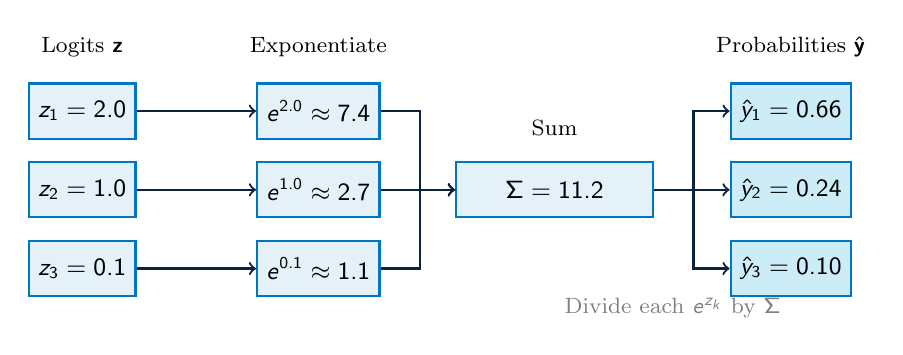
\begin{tikzpicture}[
    node distance=0.8cm,
    box/.style={rectangle, draw=tudelftblue, fill=tudelftblue!10, thick, minimum width=1.2cm, minimum height=0.7cm, font=\small},
    arrow/.style={->, thick, tudelftdarkblue},
    label/.style={font=\footnotesize}
]
    % Input logits
    \node[box] (z1) at (0, 2) {$z_1 = 2.0$};
    \node[box] (z2) at (0, 1) {$z_2 = 1.0$};
    \node[box] (z3) at (0, 0) {$z_3 = 0.1$};
    \node[label, above=0.2cm of z1] {Logits $\mathbf{z}$};
    
    % Exp
    \node[box] (e1) at (3, 2) {$e^{2.0} \approx 7.4$};
    \node[box] (e2) at (3, 1) {$e^{1.0} \approx 2.7$};
    \node[box] (e3) at (3, 0) {$e^{0.1} \approx 1.1$};
    \node[label, above=0.2cm of e1] {Exponentiate};
    
    % Sum
    \node[box, minimum width=2.5cm] (sum) at (6, 1) {$\Sigma = 11.2$};
    \node[label, above=0.2cm of sum] {Sum};
    
    % Output probabilities
    \node[box, fill=tudelftcyan!20] (p1) at (9, 2) {$\hat{y}_1 = 0.66$};
    \node[box, fill=tudelftcyan!20] (p2) at (9, 1) {$\hat{y}_2 = 0.24$};
    \node[box, fill=tudelftcyan!20] (p3) at (9, 0) {$\hat{y}_3 = 0.10$};
    \node[label, above=0.2cm of p1] {Probabilities $\hat{\mathbf{y}}$};
    
    % Arrows
    \draw[arrow] (z1) -- (e1);
    \draw[arrow] (z2) -- (e2);
    \draw[arrow] (z3) -- (e3);
    
    \draw[arrow] (e1.east) -- ++(0.5, 0) |- (sum.west);
    \draw[arrow] (e2) -- (sum);
    \draw[arrow] (e3.east) -- ++(0.5, 0) |- (sum.west);
    
    \draw[arrow] (sum.east) -- ++(0.5, 0) |- (p1.west);
    \draw[arrow] (sum.east) -- ++(0.5, 0) |- (p2.west);
    \draw[arrow] (sum.east) -- ++(0.5, 0) |- (p3.west);
    
    % Division annotation
    \node[label, text=gray] at (7.5, -0.5) {Divide each $e^{z_k}$ by $\Sigma$};
\end{tikzpicture}
\caption{The Softmax function transforms raw logits into a valid probability distribution. All outputs are positive (due to $\exp$) and sum to 1 (due to normalization). The largest logit gets the highest probability.}
\label{fig:softmax_flow}
\end{figure}

Key properties of Softmax:
\begin{itemize}
	\item All outputs are \textbf{positive} (due to exponentials) and \textbf{sum to 1} (due to normalization).
	\item It is a \textbf{soft} version of the $\arg\max$: if one logit is much larger than the others, its probability approaches 1.
	\item It is a generalization of the Sigmoid: for $K=2$, $\text{softmax}(z_1, z_2)_1 = \sigma(z_1 - z_2)$.
\end{itemize}

\subsubsection{Categorical Cross-Entropy Loss}
For multiclass classification, the negative log-likelihood of the Categorical distribution gives the \textbf{Categorical Cross-Entropy} loss:
\begin{equation}
	L_{\text{CCE}}(\hat{\mathbf{y}}, \mathbf{y}) = -\sum_{k=1}^{K} y_k \log \hat{y}_k = -\mathbf{y}^T \log \hat{\mathbf{y}}
\end{equation}
Since only one entry of $\mathbf{y}$ is 1 (for the true class $c$), this simplifies to:
\begin{equation}
	L_{\text{CCE}} = -\log \hat{y}_c
\end{equation}
The loss is simply the negative log-probability assigned to the correct class.

\subsection{Summary of Output Units and Loss Functions}
The choice of output activation and loss function are tightly coupled, determined by the task:

\begin{table}[H]
\centering
\begin{tblr}{
  colspec = {l l l l},
  row{1} = {font=\bfseries},
  hline{1,2,Z} = {solid},
}
Task & Output Activation & Loss Function & Output Distribution \\
Binary Classification & Sigmoid & Binary Cross-Entropy & Bernoulli \\
Multiclass Classification & Softmax & Categorical Cross-Entropy & Categorical \\
Regression & Linear (none) & Mean Squared Error & Gaussian \\
\end{tblr}
\caption{Summary of common output units and their corresponding loss functions, derived from the principle of maximum likelihood.}
\label{tab:loss_summary}
\end{table}

\section{Backpropagation}
\label{sec:dl_backprop}

We have established that training a neural network means minimizing a loss function $L(\boldsymbol{\theta})$, and that gradient descent requires computing $\nabla_{\boldsymbol{\theta}} L$, i.e. the gradient of the loss with respect to \textit{every} learnable parameter. In a modern network with millions of parameters, how do we compute these gradients efficiently?

\textbf{Backpropagation} (short for ``backward propagation of errors'') is the answer. It is not a new optimization algorithm, but rather a highly efficient method for computing gradients by cleverly applying the \textbf{chain rule of calculus} to the \textbf{computational graph} of the network. It powers virtually all of modern deep learning.

\subsection{The Chain Rule of Calculus}
Recall that a deep network is a composition of functions: $f(\mathbf{x}) = f^{(L)}( f^{(L-1)}( \cdots f^{(1)}(\mathbf{x}) \cdots ))$. To find how the loss changes with respect to a parameter deep inside the network, we need to trace how changes propagate through all the intermediate functions.

\paragraph{Single Variable Chain Rule:}
If $y = g(x)$ and $z = f(y) = f(g(x))$, then:
\begin{equation}
	\frac{dz}{dx} = \frac{dz}{dy} \cdot \frac{dy}{dx}
\end{equation}
The derivative of the composition is the product of the individual derivatives.

\paragraph{Multivariate Chain Rule:}
If a variable $x$ influences the output $L$ through multiple intermediate paths, we must sum the contributions from each path. If $L$ depends on $y_1, y_2, \ldots, y_n$, and each $y_i$ depends on $x$, then:
\begin{equation}
	\frac{\partial L}{\partial x} = \sum_{i=1}^{n} \frac{\partial L}{\partial y_i} \cdot \frac{\partial y_i}{\partial x}
\end{equation}
This is the key formula for backpropagation: the gradient with respect to a node is the sum of gradients flowing back from all its children.

\subsection{Computational Graphs}
To systematically apply the chain rule, we represent the network as a \textbf{computational graph}, a directed acyclic graph (DAG) where:
\begin{itemize}
	\item \textbf{Nodes} represent variables (scalars, vectors, matrices, tensors).
	\item \textbf{Edges} represent operations: an edge from $x$ to $y$ means $y$ is computed from $x$.
\end{itemize}

\begin{figure}[H]
\centering
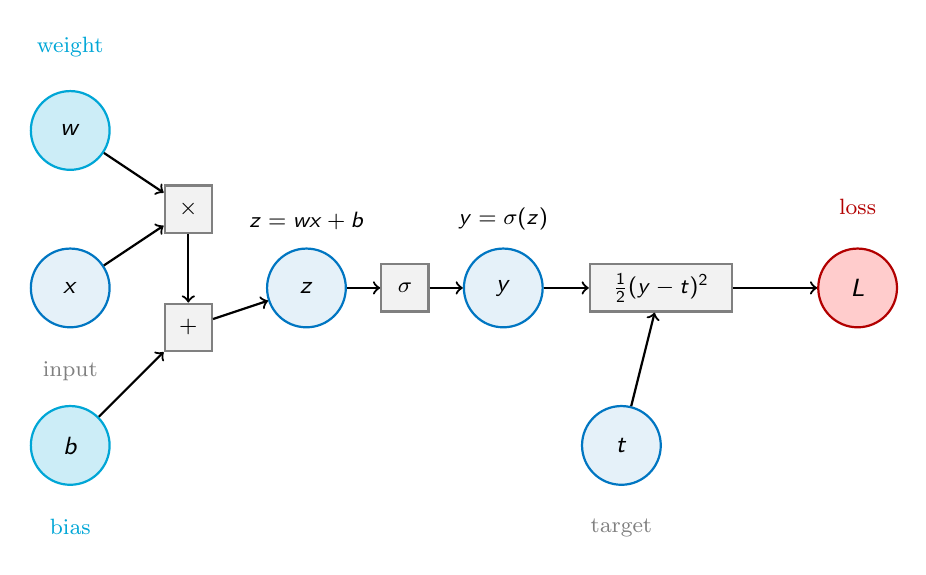
\begin{tikzpicture}[
    node distance=1.5cm,
    var/.style={circle, draw=tudelftblue, fill=tudelftblue!10, thick, minimum size=1cm, font=\small},
    param/.style={circle, draw=tudelftcyan, fill=tudelftcyan!20, thick, minimum size=1cm, font=\small},
    loss/.style={circle, draw=red!70!black, fill=red!20, thick, minimum size=1cm, font=\small},
    op/.style={rectangle, draw=gray, fill=gray!10, thick, minimum size=0.6cm, font=\footnotesize},
    opwide/.style={rectangle, draw=gray, fill=gray!10, thick, minimum width=1.8cm, minimum height=0.6cm, font=\footnotesize},
    arrow/.style={->, thick}
]
    % Input and parameters
    \node[var] (x) at (0, 0) {$x$};
    \node[param] (w) at (0, 2) {$w$};
    \node[param] (b) at (0, -2) {$b$};
    
    % z = wx + b
    \node[var] (z) at (3, 0) {$z$};
    \node[op] (mult) at (1.5, 1) {$\times$};
    \node[op] (add) at (1.5, -0.5) {$+$};
    
    % y = sigma(z)
    \node[var] (y) at (5.5, 0) {$y$};
    \node[op] (sig) at (4.25, 0) {$\sigma$};
    
    % t (target)
    \node[var] (t) at (7, -2) {$t$};
    
    % Loss - spread out more
    \node[loss] (L) at (10, 0) {$L$};
    \node[opwide] (lossfn) at (7.5, 0) {$\tfrac{1}{2}(y - t)^2$};
    
    % Forward arrows
    \draw[arrow] (x) -- (mult);
    \draw[arrow] (w) -- (mult);
    \draw[arrow] (mult) -- (add);
    \draw[arrow] (b) -- (add);
    \draw[arrow] (add) -- (z);
    \draw[arrow] (z) -- (sig);
    \draw[arrow] (sig) -- (y);
    \draw[arrow] (y) -- (lossfn);
    \draw[arrow] (t) -- (lossfn);
    \draw[arrow] (lossfn) -- (L);
    
    % Labels
    \node[below=0.3cm of x, font=\footnotesize, text=gray] {input};
    \node[above=0.3cm of w, font=\footnotesize, text=tudelftcyan] {weight};
    \node[below=0.3cm of b, font=\footnotesize, text=tudelftcyan] {bias};
    \node[below=0.3cm of t, font=\footnotesize, text=gray] {target};
    \node[above=0.3cm of L, font=\footnotesize, text=red!70!black] {loss};
    
    % Annotations for z
    \node[above=0.1cm of z, font=\footnotesize] {$z = wx + b$};
    \node[above=0.1cm of y, font=\footnotesize] {$y = \sigma(z)$};
\end{tikzpicture}
\caption{A computational graph for logistic regression with squared error loss. Blue nodes are inputs/intermediate values, cyan nodes are learnable parameters ($w$, $b$), and the red node is the loss. Edges show the flow of computation during the forward pass.}
\label{fig:comp_graph_forward}
\end{figure}

\subsection{Forward Pass and Backward Pass}
The backpropagation algorithm consists of two phases:

\paragraph{1. Forward Pass:}
Starting from the inputs, compute and cache the value of every node in topological order (parents before children) until we reach the loss $L$. This is simply running the network to get a prediction.

\paragraph{2. Backward Pass:}
Starting from the loss, compute the gradient of $L$ with respect to every node in \textit{reverse} topological order (children before parents). We use the chain rule: the gradient of a node is the sum of gradients flowing back from all its children, each multiplied by the local derivative.

Let $\bar{n} = \frac{\partial L}{\partial n}$ denote the gradient of the loss with respect to node $n$ (``bar notation''). The backward pass computes:
\begin{equation}
	\bar{n} = \sum_{c \in \text{Children}(n)} \bar{c} \cdot \frac{\partial c}{\partial n}
\end{equation}
where ``Children($n$)'' are all nodes that directly depend on $n$.

\subsection{Worked Example: Logistic Regression}
Consider the model $L = \frac{1}{2}(y - t)^2$, where $y = \sigma(z)$ and $z = wx + b$. We want $\frac{\partial L}{\partial w}$ and $\frac{\partial L}{\partial b}$.

\subsubsection{The Naïve Approach}
Directly applying the chain rule from scratch for each parameter:
\begin{align}
	\frac{\partial L}{\partial w} &= \frac{\partial}{\partial w} \left[ \frac{1}{2}(\sigma(wx+b) - t)^2 \right] \\
	&= (\sigma(wx+b) - t) \cdot \sigma'(wx+b) \cdot x
\end{align}
Similarly for $b$. The problem: we recompute many sub-expressions (like $\sigma'(wx+b)$) multiple times. For deep networks, this redundancy leads to \textbf{exponential complexity}.

\subsubsection{The Backpropagation Approach}
Decompose the computation into elementary steps and reuse intermediate gradients.

\textbf{Forward Pass:} Compute and store:
\begin{align}
	z &= wx + b \\
	y &= \sigma(z) \\
	L &= \frac{1}{2}(y - t)^2
\end{align}

\textbf{Backward Pass (using bar notation $\bar{n} = \frac{\partial L}{\partial n}$):}
\begin{enumerate}
	\item $\bar{L} = 1$ \quad (gradient of loss w.r.t. itself)
	\item $\bar{y} = \bar{L} \cdot \frac{\partial L}{\partial y} = 1 \cdot (y - t) = y - t$
	\item $\bar{z} = \bar{y} \cdot \frac{\partial y}{\partial z} = (y - t) \cdot \sigma'(z)$
	\item $\bar{w} = \bar{z} \cdot \frac{\partial z}{\partial w} = \bar{z} \cdot x$ \quad $\leftarrow$ \textbf{This is $\frac{\partial L}{\partial w}$}
	\item $\bar{b} = \bar{z} \cdot \frac{\partial z}{\partial b} = \bar{z} \cdot 1 = \bar{z}$ \quad $\leftarrow$ \textbf{This is $\frac{\partial L}{\partial b}$}
\end{enumerate}

Notice that $\bar{z}$ is computed \textit{once} and reused to compute both $\bar{w}$ and $\bar{b}$. This reuse is what makes backpropagation efficient: we only compute each intermediate gradient once, achieving \textbf{linear complexity} in the number of nodes.

\begin{figure}[H]
\centering
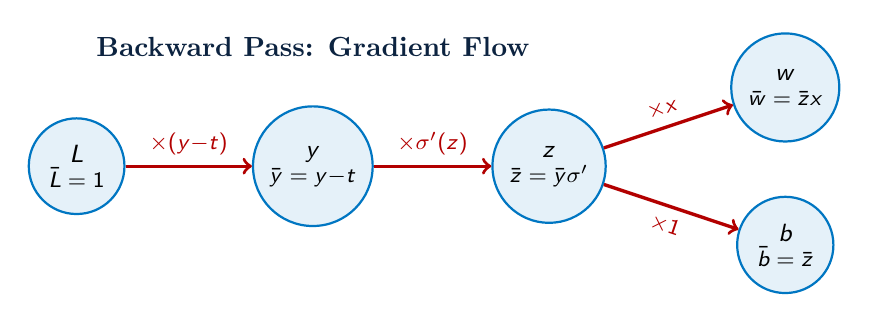
\begin{tikzpicture}[
    node distance=1.8cm,
    var/.style={circle, draw=tudelftblue, fill=tudelftblue!10, thick, minimum size=1.2cm, font=\small, align=center},
    arrow/.style={->, very thick, red!70!black},
    label/.style={font=\footnotesize, text=red!70!black}
]
    % Nodes
    \node[var] (L) at (0, 0) {$L$\\[-2pt]\footnotesize$\bar{L}=1$};
    \node[var] (y) at (3, 0) {$y$\\[-2pt]\footnotesize$\bar{y}=y{-}t$};
    \node[var] (z) at (6, 0) {$z$\\[-2pt]\footnotesize$\bar{z}=\bar{y}\sigma'$};
    \node[var] (w) at (9, 1) {$w$\\[-2pt]\footnotesize$\bar{w}=\bar{z}x$};
    \node[var] (b) at (9, -1) {$b$\\[-2pt]\footnotesize$\bar{b}=\bar{z}$};
    
    % Backward arrows (reversed direction, showing gradient flow)
    \draw[arrow] (L) -- node[above, label] {$\times(y{-}t)$} (y);
    \draw[arrow] (y) -- node[above, label] {$\times\sigma'(z)$} (z);
    \draw[arrow] (z) -- node[above, label, sloped] {$\times x$} (w);
    \draw[arrow] (z) -- node[below, label, sloped] {$\times 1$} (b);
    
    % Title
    \node[above=0.5cm of y, font=\bfseries, text=tudelftdarkblue] {Backward Pass: Gradient Flow};
\end{tikzpicture}
\caption{Gradient flow in the backward pass. Starting from $\bar{L} = 1$, we propagate gradients backwards, multiplying by local derivatives at each step. The gradient $\bar{z}$ is computed once and reused for both $\bar{w}$ and $\bar{b}$.}
\label{fig:backprop_flow}
\end{figure}

\subsection{Modularity: Local Gradients}
A beautiful property of backpropagation is its \textbf{modularity}. Each node in the computational graph only needs to know:
\begin{enumerate}
	\item How to compute its output given its inputs (for the forward pass).
	\item How to compute the gradient with respect to its inputs, given the gradient with respect to its output (for the backward pass).
\end{enumerate}
This is why deep learning frameworks like PyTorch and TensorFlow can automatically differentiate arbitrary compositions of operations: each operation is a module that defines its own forward and backward functions. You can compose modules freely, and the framework handles the gradient computation.

\begin{table}[H]
\centering
\begin{tblr}{
  colspec = {l l l},
  row{1} = {font=\bfseries},
  hline{1,2,Z} = {solid},
}
Operation & Forward: $y = f(x)$ & Backward: $\bar{x} = \bar{y} \cdot \frac{\partial y}{\partial x}$ \\
Addition: $y = x_1 + x_2$ & $y = x_1 + x_2$ & $\bar{x}_1 = \bar{y}$, $\bar{x}_2 = \bar{y}$ \\
Multiplication: $y = x_1 \cdot x_2$ & $y = x_1 \cdot x_2$ & $\bar{x}_1 = \bar{y} \cdot x_2$, $\bar{x}_2 = \bar{y} \cdot x_1$ \\
ReLU: $y = \max(0, x)$ & $y = \max(0, x)$ & $\bar{x} = \bar{y} \cdot \mathbf{1}_{x > 0}$ \\
Sigmoid: $y = \sigma(x)$ & $y = \frac{1}{1+e^{-x}}$ & $\bar{x} = \bar{y} \cdot y(1-y)$ \\
\end{tblr}
\caption{Examples of local forward and backward rules for common operations. Each operation only needs to know its own local derivative. The framework chains these together using the chain rule.}
\label{tab:local_gradients}
\end{table}

\subsection{Complexity Analysis}
\paragraph{Naïve Approach:} Computing each parameter's gradient independently requires tracing back through the entire graph for each parameter, leading to $O(N \cdot M)$ complexity where $N$ is the number of nodes and $M$ is the number of parameters.

\paragraph{Backpropagation:} By caching and reusing intermediate gradients, backpropagation computes \textit{all} gradients in a single backward pass with $O(N)$ complexity (the same order as the forward pass). This is an enormous saving for networks with millions of parameters.


\section{Optimization Algorithms}
\label{sec:dl_optimization}

We have a loss function and we know how to compute its gradient via backpropagation. The final ingredient is an algorithm to actually update the parameters. While vanilla Stochastic Gradient Descent (SGD) is the conceptual foundation, its noisy updates can lead to slow, oscillating convergence. Modern optimizers leverage \textbf{past gradient statistics} to smooth out noise and accelerate training.

\subsection{The Problem with Vanilla SGD}
Recall the SGD update rule for a mini-batch of $k$ samples:
\begin{equation}
	\boldsymbol{\theta}_{t+1} = \boldsymbol{\theta}_t - \eta \cdot \frac{1}{k} \sum_{i=1}^{k} \nabla_{\boldsymbol{\theta}} L(\mathbf{x}^{(i)}, y^{(i)}; \boldsymbol{\theta}_t)
\end{equation}
where $\eta$ is the learning rate. The key issue is that the mini-batch gradient is a \textit{noisy estimate} of the true gradient over the full dataset. This stochasticity is a blessing (it enables training on huge datasets and can help escape local minima) but also a curse:
\begin{itemize}
	\item \textbf{Oscillations in ravines:} When the loss surface is much steeper in one direction than another (an elongated ``ravine''), SGD oscillates back and forth across the steep direction while making slow progress along the shallow direction.
	\item \textbf{Learning rate sensitivity:} A learning rate that is too high causes divergence; too low causes painfully slow convergence.
\end{itemize}

\subsection{Exponentially Weighted Moving Average (EWMA)}
The solution is to smooth out the noisy gradient estimates using their history. A naïve approach of storing all past gradients is infeasible for networks with millions of parameters. Instead, we use the \textbf{Exponentially Weighted Moving Average (EWMA)}, an elegant recursive formula that summarizes history in a single vector:
\begin{equation}
	v_t = \rho \cdot v_{t-1} + (1 - \rho) \cdot g_t
\end{equation}
where $g_t$ is the current gradient, $v_t$ is the smoothed average, and $\rho \in [0, 1)$ is the \textbf{decay rate} controlling how much history to retain. A higher $\rho$ means more smoothing (longer memory).

\paragraph{Bias Correction:} Initializing $v_0 = 0$ biases the estimate towards zero in early iterations. We correct this:
\begin{equation}
	\hat{v}_t = \frac{v_t}{1 - \rho^t}
\end{equation}
As $t \to \infty$, the correction factor $1 - \rho^t \to 1$, so it only matters at the start.

\begin{figure}[H]
\begin{pycode}
# Exponential Weighted Moving Average (EWMA) Visualization
np.random.seed(42)
T = 100
t_arr = np.arange(1, T + 1)
# Generate noisy data: True signal is 1, plus noise
true_signal = np.ones(T)
noise = np.random.normal(0, 0.5, T)
y = true_signal + noise

# EWMA Calculation
rho = 0.9
v = np.zeros(T)
v_corrected = np.zeros(T)
current_v = 0

for i in range(T):
    current_v = rho * current_v + (1 - rho) * y[i]
    v[i] = current_v
    # Bias correction
    v_corrected[i] = current_v / (1 - rho**(i + 1))

fig, ax = plt.subplots(figsize=(10, 5))

# Plot Raw Noisy Data
ax.plot(t_arr, y, 'o', color=utils.COLORS['gray'], alpha=0.4, label=r'Noisy Gradients ($g_t$)', markersize=4)

# Plot Uncorrected EWMA
ax.plot(t_arr, v, '--', color=utils.COLORS['red'], linewidth=2, label=rf'EWMA ($\rho={rho}$, No Bias Corr.)')

# Plot Corrected EWMA
ax.plot(t_arr, v_corrected, '-', color=utils.COLORS['primary'], linewidth=2.5, label=rf'EWMA ($\rho={rho}$, Bias Corrected)')

ax.axhline(1.0, color='black', linestyle=':', label='True Mean')

ax.set_title('Smoothing Noisy Signals with EWMA')
ax.set_xlabel('Iteration ($t$)')
ax.set_ylabel('Value')
ax.legend(loc='lower right')
ax.grid(True, linestyle=':', alpha=0.6)

utils.save_and_include("ewma_bias_correction.pdf", width=r"0.9\textwidth")
\end{pycode}
\caption{EWMA and Bias Correction. The noisy gradients (gray dots) are smoothed. Without bias correction (red dashed), the estimate starts near zero. With bias correction (blue solid), the estimate tracks the true mean from the beginning.}
\label{fig:ewma_bias_correction}
\end{figure}

\subsection{Momentum}
\textbf{Momentum} applies EWMA directly to the gradient, accumulating a ``velocity'' vector that smooths out oscillations and accelerates motion in consistent directions:

\begin{tcolorbox}[colback=tudelftblue!5!white, colframe=tudelftblue, title=SGD with Momentum]
\textbf{Initialize:} $\mathbf{v}_0 = \mathbf{0}$

\textbf{At each iteration $t$:}
\begin{enumerate}
	\item Compute gradient: $\mathbf{g}_t = \nabla_{\boldsymbol{\theta}} L(\boldsymbol{\theta}_{t-1})$
	\item Update velocity: $\mathbf{v}_t = \rho \cdot \mathbf{v}_{t-1} + (1 - \rho) \cdot \mathbf{g}_t$
	\item Update parameters: $\boldsymbol{\theta}_t = \boldsymbol{\theta}_{t-1} - \eta \cdot \mathbf{v}_t$
\end{enumerate}
\textbf{Typical hyperparameter:} $\rho = 0.9$
\end{tcolorbox}

The intuition: imagine a ball rolling down a hill. It doesn't just follow the local gradient; it builds up speed. If the gradient consistently points in one direction, the velocity grows. If it oscillates, the velocity damps out. This allows Momentum to traverse ravines efficiently.

\subsection{RMSprop}
While Momentum smooths the \textit{direction} of the gradient, \textbf{RMSprop} (Root Mean Square Propagation) addresses its \textit{magnitude}. It maintains an EWMA of the \textit{squared} gradients, which estimates the variance:

\begin{tcolorbox}[colback=tudelftblue!5!white, colframe=tudelftblue, title=RMSprop]
\textbf{Initialize:} $\mathbf{r}_0 = \mathbf{0}$

\textbf{At each iteration $t$:}
\begin{enumerate}
	\item Compute gradient: $\mathbf{g}_t = \nabla_{\boldsymbol{\theta}} L(\boldsymbol{\theta}_{t-1})$
	\item Update squared gradient average: $\mathbf{r}_t = \rho \cdot \mathbf{r}_{t-1} + (1 - \rho) \cdot \mathbf{g}_t^2$ \quad (element-wise)
	\item Update parameters: $\boldsymbol{\theta}_t = \boldsymbol{\theta}_{t-1} - \frac{\eta}{\sqrt{\mathbf{r}_t} + \epsilon} \odot \mathbf{g}_t$
\end{enumerate}
\textbf{Typical hyperparameters:} $\rho = 0.99$, $\epsilon = 10^{-8}$ (for numerical stability)
\end{tcolorbox}

The key insight: dividing by $\sqrt{\mathbf{r}_t}$ \textit{normalizes} the update. Parameters with large, variable gradients get smaller updates (preventing exploding steps), while parameters with small, consistent gradients get larger updates (accelerating through flat regions). RMSprop adapts the learning rate \textit{per-parameter}.

\subsection{Adam (Adaptive Moment Estimation)}
\textbf{Adam} combines the best of both worlds: Momentum's smoothed gradient direction and RMSprop's per-parameter adaptive learning rate. It is currently the \textbf{default optimizer} for most deep learning applications.

\begin{tcolorbox}[colback=tudelftblue!5!white, colframe=tudelftblue, title=Adam Optimizer]
\textbf{Initialize:} $\mathbf{m}_0 = \mathbf{0}$ (first moment), $\mathbf{v}_0 = \mathbf{0}$ (second moment)

\textbf{At each iteration $t$:}
\begin{enumerate}
	\item Compute gradient: $\mathbf{g}_t = \nabla_{\boldsymbol{\theta}} L(\boldsymbol{\theta}_{t-1})$
	\item Update first moment (mean): $\mathbf{m}_t = \beta_1 \cdot \mathbf{m}_{t-1} + (1 - \beta_1) \cdot \mathbf{g}_t$
	\item Update second moment (variance): $\mathbf{v}_t = \beta_2 \cdot \mathbf{v}_{t-1} + (1 - \beta_2) \cdot \mathbf{g}_t^2$
	\item Bias correction: $\hat{\mathbf{m}}_t = \frac{\mathbf{m}_t}{1 - \beta_1^t}$, \quad $\hat{\mathbf{v}}_t = \frac{\mathbf{v}_t}{1 - \beta_2^t}$
	\item Update parameters: $\boldsymbol{\theta}_t = \boldsymbol{\theta}_{t-1} - \frac{\eta \cdot \hat{\mathbf{m}}_t}{\sqrt{\hat{\mathbf{v}}_t} + \epsilon}$
\end{enumerate}
\textbf{Default hyperparameters:} $\beta_1 = 0.9$, $\beta_2 = 0.999$, $\epsilon = 10^{-8}$
\end{tcolorbox}

\subsection{Summary of Optimizers}

\begin{table}[H]
\centering
\begin{tblr}{
  colspec = {l l X[l]},
  row{1} = {font=\bfseries},
  hline{1,2,Z} = {solid},
}
Optimizer & Tracks & Key Benefit \\
SGD & --- & Simple baseline \\
Momentum & EWMA of $\mathbf{g}$ (first moment) & Smooths direction, accelerates in consistent directions \\
RMSprop & EWMA of $\mathbf{g}^2$ (second moment) & Adapts learning rate per-parameter \\
Adam & Both first and second moments & Combines benefits of Momentum and RMSprop \\
\end{tblr}
\caption{Comparison of optimization algorithms.}
\label{tab:optimizer_comparison}
\end{table}

\paragraph{Practical Note: Learning Rate Sensitivity.}
Different optimizers require different learning rates to converge effectively. SGD typically needs careful tuning (often $0.01$--$0.1$), while Adam is more forgiving due to its adaptive per-parameter rates (default $\eta = 0.001$ works well in many cases). When switching optimizers, always re-tune the learning rate.

\paragraph{Weight Decay and L2 Regularization.}
In frameworks like PyTorch, the \texttt{weight\_decay} parameter in optimizers is simply L2 regularization implemented within the update rule. Setting \texttt{weight\_decay=0.01} is equivalent to adding $\frac{0.01}{2}\|\boldsymbol{\theta}\|^2$ to the loss. This penalizes large weights and encourages simpler models.

\paragraph{Early Stopping.}
Rather than training for a fixed number of epochs, we can halt training when the model begins to overfit. We monitor the validation loss (or accuracy) and stop when it fails to improve for a set number of epochs (called \textbf{patience}). This acts as a form of regularization: the model is prevented from memorizing the training set. In practice, we save the best model checkpoint and restore it after training ends.
\section{Normalization Techniques}
\label{sec:dl_normalization}

Optimization is significantly easier when the loss landscape is \textbf{well-conditioned}---spherical rather than elongated. Normalizing the inputs to have zero mean and unit variance is a well-known preprocessing step. But what about the hidden layers?

\subsection{The Internal Covariate Shift Problem}
As a deep network trains, the distribution of activations in each hidden layer changes continuously because the parameters of preceding layers are being updated. This phenomenon, called \textbf{Internal Covariate Shift}, forces each layer to constantly adapt to new input distributions, slowing down training.

\subsection{Batch Normalization}
\textbf{Batch Normalization (BatchNorm)} addresses this by normalizing the activations within each mini-batch. For a layer with pre-activation $\mathbf{z}$, given a mini-batch $\mathcal{B}$ of size $m$:

\begin{enumerate}
	\item \textbf{Compute batch statistics:}
	\begin{equation}
		\mu_{\mathcal{B}} = \frac{1}{m} \sum_{i=1}^{m} z_i, \qquad \sigma_{\mathcal{B}}^2 = \frac{1}{m} \sum_{i=1}^{m} (z_i - \mu_{\mathcal{B}})^2
	\end{equation}
	\item \textbf{Normalize:}
	\begin{equation}
		\hat{z}_i = \frac{z_i - \mu_{\mathcal{B}}}{\sqrt{\sigma_{\mathcal{B}}^2 + \epsilon}}
	\end{equation}
	where $\epsilon$ (e.g., $10^{-8}$) prevents division by zero.
	\item \textbf{Scale and shift} (learnable parameters $\gamma$, $\beta$):
	\begin{equation}
		y_i = \gamma \hat{z}_i + \beta
	\end{equation}
\end{enumerate}

The learnable parameters $\gamma$ and $\beta$ are crucial: they allow the network to \textit{undo} the normalization if that is optimal, restoring the representational power. In fact, setting $\gamma = \sigma_{\mathcal{B}}$ and $\beta = \mu_{\mathcal{B}}$ recovers the original activations.

\begin{figure}[H]
\centering
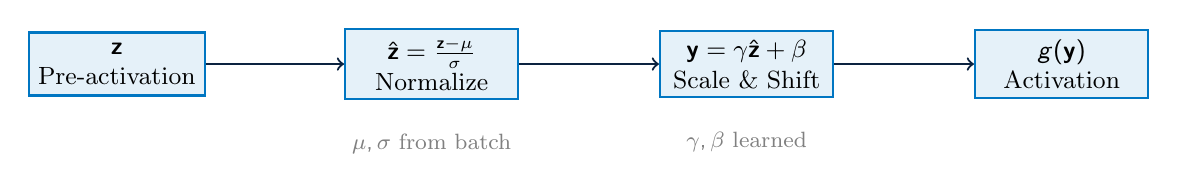
\begin{tikzpicture}[
    block/.style={rectangle, draw=tudelftblue, fill=tudelftblue!10, thick, minimum width=2.2cm, minimum height=0.8cm, font=\small, align=center},
    arrow/.style={->, thick, tudelftdarkblue},
    label/.style={font=\footnotesize, text=gray}
]
    % Nodes
    \node[block] (z) at (0, 0) {$\mathbf{z}$\\Pre-activation};
    \node[block] (norm) at (4, 0) {$\hat{\mathbf{z}} = \frac{\mathbf{z} - \mu}{\sigma}$\\Normalize};
    \node[block] (scale) at (8, 0) {$\mathbf{y} = \gamma\hat{\mathbf{z}} + \beta$\\Scale \& Shift};
    \node[block] (act) at (12, 0) {$g(\mathbf{y})$\\Activation};
    
    % Arrows
    \draw[arrow] (z) -- (norm);
    \draw[arrow] (norm) -- (scale);
    \draw[arrow] (scale) -- (act);
    
    % Annotations
    \node[label, below=0.3cm of norm] {$\mu, \sigma$ from batch};
    \node[label, below=0.3cm of scale] {$\gamma, \beta$ learned};
\end{tikzpicture}
\caption{Batch Normalization pipeline. The pre-activations are normalized using batch statistics, then scaled and shifted by learnable parameters before being passed through the activation function.}
\label{fig:batchnorm_pipeline}
\end{figure}

\paragraph{Inference Time:} At test time, we don't have a batch to compute statistics from. Instead, we use \textbf{running averages} of $\mu$ and $\sigma^2$ accumulated during training (using EWMA, our friend from optimization!).

\paragraph{Where to Apply BatchNorm:} There is some debate, but the common practice is to apply BatchNorm \textit{before} the activation function: $\text{Activation}(\text{BatchNorm}(\mathbf{W}\mathbf{x} + \mathbf{b}))$. Note that the bias $\mathbf{b}$ becomes redundant since BatchNorm has its own learnable shift $\beta$.


\section{Convolutional Neural Networks (CNNs)}
\label{sec:dl_cnn}

Deep Feedforward Networks are powerful universal function approximators, but they face a fundamental challenge with high-dimensional structured data like images. Consider a modest $256 \times 256$ RGB image: a fully connected layer would have $256 \times 256 \times 3 = 196,608$ input units. Connecting this to just 1,000 hidden units requires nearly 200 million parameters, and that's just the first layer! This is computationally intractable and extremely prone to overfitting.

\textbf{Convolutional Neural Networks (CNNs)} solve this problem by encoding strong \textbf{prior knowledge} about the structure of images:
\begin{enumerate}
	\item \textbf{Locality}: Nearby pixels are strongly correlated (a sky pixel is likely surrounded by other sky pixels). Distant pixels are often unrelated.
	\item \textbf{Translation Equivariance}: An object (e.g., a cat) is the same object regardless of where it appears in the image. The features that detect it should be shared across all positions.
\end{enumerate}

\subsection{The Convolution Operation}
The core building block of CNNs is the \textbf{convolution} (technically, a cross-correlation). Instead of connecting every input to every output, we slide a small \textbf{kernel} (or filter) $\mathbf{K}$ over the input image $\mathbf{I}$, computing a dot product at each position:
\begin{equation}
	(\mathbf{I} * \mathbf{K})(i, j) = \sum_{m=0}^{k-1} \sum_{n=0}^{k-1} \mathbf{I}(i+m, j+n) \cdot \mathbf{K}(m, n)
\end{equation}
where $k$ is the kernel size (e.g., $3 \times 3$). This produces an \textbf{output feature map} (or activation map).

\begin{figure}[H]
\centering
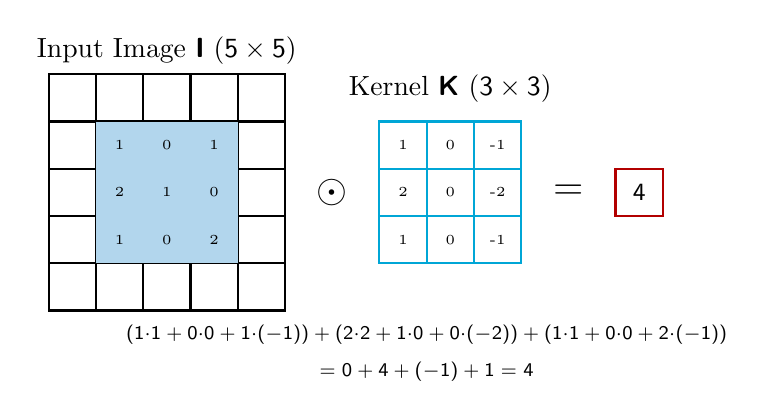
\begin{tikzpicture}[scale=0.6]
    % Input image (5x5 grid)
    \foreach \i in {0,...,4} {
        \foreach \j in {0,...,4} {
            \draw[thick] (\i, -\j) rectangle (\i+1, -\j-1);
        }
    }
    \node at (2.5, 0.5) {Input Image $\mathbf{I}$ ($5 \times 5$)};
    
    % Highlight the receptive field (3x3 at position 1,1)
    \fill[tudelftblue!30] (1, -1) rectangle (4, -4);
    
    % Sample values in receptive field
    \node[font=\tiny] at (1.5, -1.5) {1};
    \node[font=\tiny] at (2.5, -1.5) {0};
    \node[font=\tiny] at (3.5, -1.5) {1};
    \node[font=\tiny] at (1.5, -2.5) {2};
    \node[font=\tiny] at (2.5, -2.5) {1};
    \node[font=\tiny] at (3.5, -2.5) {0};
    \node[font=\tiny] at (1.5, -3.5) {1};
    \node[font=\tiny] at (2.5, -3.5) {0};
    \node[font=\tiny] at (3.5, -3.5) {2};
    
    % Multiplication symbol
    \node at (6, -2.5) {\Large $\odot$};
    
    % Kernel (3x3)
    \foreach \i in {0,...,2} {
        \foreach \j in {0,...,2} {
            \draw[thick, tudelftcyan] (7+\i, -1-\j) rectangle (8+\i, -2-\j);
        }
    }
    \node at (8.5, -0.3) {Kernel $\mathbf{K}$ ($3 \times 3$)};
    
    % Kernel values
    \node[font=\tiny] at (7.5, -1.5) {1};
    \node[font=\tiny] at (8.5, -1.5) {0};
    \node[font=\tiny] at (9.5, -1.5) {-1};
    \node[font=\tiny] at (7.5, -2.5) {2};
    \node[font=\tiny] at (8.5, -2.5) {0};
    \node[font=\tiny] at (9.5, -2.5) {-2};
    \node[font=\tiny] at (7.5, -3.5) {1};
    \node[font=\tiny] at (8.5, -3.5) {0};
    \node[font=\tiny] at (9.5, -3.5) {-1};
    
    % Equals
    \node at (11, -2.5) {\Large $=$};
    
    % Output (single value in context of 3x3 output)
    \draw[thick, red!70!black] (12, -2) rectangle (13, -3);
    \node[font=\small] at (12.5, -2.5) {$4$};
    
    % Calculation below
    \node[font=\scriptsize, align=left] at (8, -5.5) {$(1{\cdot}1 + 0{\cdot}0 + 1{\cdot}(-1)) + (2{\cdot}2 + 1{\cdot}0 + 0{\cdot}(-2)) + (1{\cdot}1 + 0{\cdot}0 + 2{\cdot}(-1))$};
    \node[font=\scriptsize] at (8, -6.3) {$= 0 + 4 + (-1) + 1 = 4$};
\end{tikzpicture}
\caption{The convolution operation. A $3 \times 3$ kernel slides over the input. At each position, we compute the element-wise product and sum all values to produce one output. The highlighted blue region shows the \textbf{receptive field} for one output pixel.}
\label{fig:conv_operation}
\end{figure}

\paragraph{Key Properties of Convolution:}
\begin{itemize}
	\item \textbf{Sparse Interactions:} Each output depends on only a small local region of the input (the kernel size), not the entire image. This drastically reduces parameters.
	\item \textbf{Parameter Sharing:} The same kernel weights $\mathbf{K}$ are used at every spatial position. We don't learn separate weights for the top-left vs. bottom-right of the image.
\end{itemize}

\subsection{Multiple Channels and Multiple Kernels}
Real images have multiple \textbf{input channels} (e.g., 3 for RGB). And we typically want to learn multiple different features (edges, textures, colors), requiring multiple \textbf{output channels}.

For an input with $C_{in}$ channels, the kernel is actually 3-dimensional: $(C_{in} \times k \times k)$. We sum the convolutions across all input channels to produce one output channel:
\begin{equation}
	\text{Output}(i, j) = \sum_{c=1}^{C_{in}} (\mathbf{I}_c * \mathbf{K}_c)(i, j) + b
\end{equation}
To produce $C_{out}$ output channels (feature maps), we use $C_{out}$ different kernels, each of shape $(C_{in} \times k \times k)$.

\begin{tcolorbox}[colback=tudelftblue!5!white, colframe=tudelftblue, title=Parameter Count for a Convolutional Layer]
A convolutional layer with input channels $C_{in}$, output channels $C_{out}$, and kernel size $k \times k$ has:
\begin{equation}
	\text{Parameters} = C_{out} \times (C_{in} \times k \times k + 1) = C_{out} \cdot C_{in} \cdot k^2 + C_{out}
\end{equation}
where the $+1$ accounts for a bias term per output channel. For example, a $3 \times 3$ conv from 64 to 128 channels has $128 \times 64 \times 9 + 128 = 73,856$ parameters, compared to millions for a fully connected equivalent.
\end{tcolorbox}

\subsection{Padding and Stride}
Two important hyperparameters control the spatial size of the output:

\paragraph{Padding:} Without padding, applying a $k \times k$ kernel shrinks the spatial dimensions. For an input of size $N \times N$:
\begin{equation}
	\text{Output size (valid/no padding)} = N - k + 1
\end{equation}
To maintain the same spatial size, we add \textbf{zero-padding} of $p = \lfloor k/2 \rfloor$ pixels around the border (called ``same'' padding).

\begin{figure}[H]
\centering
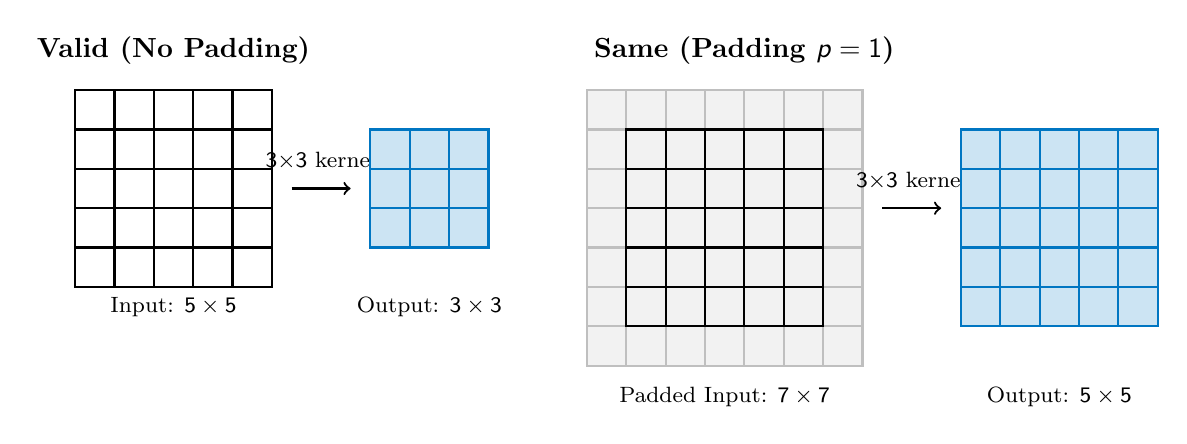
\begin{tikzpicture}[scale=0.5]
    % Valid convolution (no padding)
    \node[font=\bfseries] at (2.5, 1) {Valid (No Padding)};
    
    % Input 5x5
    \foreach \i in {0,...,4} {
        \foreach \j in {0,...,4} {
            \draw[thick] (\i, -\j) rectangle (\i+1, -\j-1);
        }
    }
    \node[font=\footnotesize] at (2.5, -5.5) {Input: $5 \times 5$};
    
    % Arrow
    \draw[->, thick] (5.5, -2.5) -- (7, -2.5);
    \node[font=\footnotesize] at (6.25, -1.8) {$3{\times}3$ kernel};
    
    % Output 3x3
    \foreach \i in {0,...,2} {
        \foreach \j in {0,...,2} {
            \draw[thick, tudelftblue, fill=tudelftblue!20] (7.5+\i, -1-\j) rectangle (8.5+\i, -2-\j);
        }
    }
    \node[font=\footnotesize] at (9, -5.5) {Output: $3 \times 3$};
    
    % Same convolution (with padding)
    \node[font=\bfseries] at (17, 1) {Same (Padding $p=1$)};
    
    % Padding (7x7)
    \foreach \i in {0,...,6} {
        \foreach \j in {0,...,6} {
            \draw[thick, gray!50, fill=gray!10] (13+\i, -\j) rectangle (14+\i, -\j-1);
        }
    }
    % Inner input 5x5
    \foreach \i in {0,...,4} {
        \foreach \j in {0,...,4} {
            \draw[thick] (14+\i, -1-\j) rectangle (15+\i, -2-\j);
        }
    }
    \node[font=\footnotesize] at (16.5, -7.8) {Padded Input: $7 \times 7$};
    
    % Arrow
    \draw[->, thick] (20.5, -3) -- (22, -3);
    \node[font=\footnotesize] at (21.25, -2.3) {$3{\times}3$ kernel};
    
    % Output 5x5
    \foreach \i in {0,...,4} {
        \foreach \j in {0,...,4} {
            \draw[thick, tudelftblue, fill=tudelftblue!20] (22.5+\i, -1-\j) rectangle (23.5+\i, -2-\j);
        }
    }
    \node[font=\footnotesize] at (25, -7.8) {Output: $5 \times 5$};
\end{tikzpicture}
\caption{\textbf{Left:} Valid convolution: no padding, output shrinks. \textbf{Right:} Same convolution: zero-padding (gray) preserves spatial dimensions.}
\label{fig:padding}
\end{figure}

\paragraph{Stride:} Instead of moving the kernel one pixel at a time, we can move it by $s$ pixels (\textbf{stride}). This downsamples the output:
\begin{equation}
	\text{Output size} = \left\lfloor \frac{N + 2p - k}{s} \right\rfloor + 1
\end{equation}
Strided convolutions are an alternative to pooling for reducing spatial dimensions.

\subsection{Pooling}
\textbf{Pooling} layers reduce the spatial dimensions by summarizing local regions:
\begin{itemize}
	\item \textbf{Max Pooling:} Takes the maximum value in each region. Retains the strongest activation.
	\item \textbf{Average Pooling:} Takes the mean value. Provides a smoother downsampling.
\end{itemize}

\begin{figure}[H]
\centering
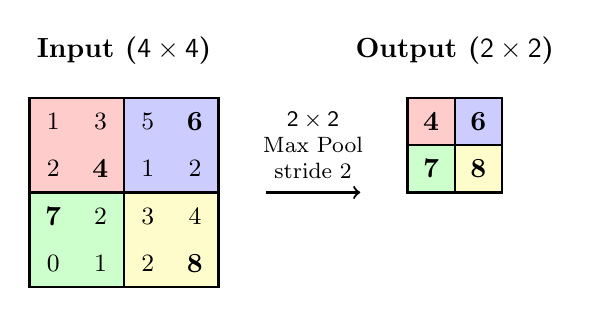
\begin{tikzpicture}[scale=0.6]
    % Input 4x4
    \node[font=\bfseries] at (2, 1) {Input ($4 \times 4$)};
    \foreach \i in {0,...,3} {
        \foreach \j in {0,...,3} {
            \draw[thick] (\i, -\j) rectangle (\i+1, -\j-1);
        }
    }
    % Fill quadrants with colors
    \fill[red!20] (0, 0) rectangle (2, -2);
    \fill[blue!20] (2, 0) rectangle (4, -2);
    \fill[green!20] (0, -2) rectangle (2, -4);
    \fill[yellow!20] (2, -2) rectangle (4, -4);
    \draw[thick] (0, 0) rectangle (4, -4);
    \draw[thick] (2, 0) -- (2, -4);
    \draw[thick] (0, -2) -- (4, -2);
    
    % Values
    \node[font=\small] at (0.5, -0.5) {1};
    \node[font=\small] at (1.5, -0.5) {3};
    \node[font=\small] at (0.5, -1.5) {2};
    \node[font=\small, font=\bfseries] at (1.5, -1.5) {4};
    
    \node[font=\small] at (2.5, -0.5) {5};
    \node[font=\small, font=\bfseries] at (3.5, -0.5) {6};
    \node[font=\small] at (2.5, -1.5) {1};
    \node[font=\small] at (3.5, -1.5) {2};
    
    \node[font=\small, font=\bfseries] at (0.5, -2.5) {7};
    \node[font=\small] at (1.5, -2.5) {2};
    \node[font=\small] at (0.5, -3.5) {0};
    \node[font=\small] at (1.5, -3.5) {1};
    
    \node[font=\small] at (2.5, -2.5) {3};
    \node[font=\small] at (3.5, -2.5) {4};
    \node[font=\small] at (2.5, -3.5) {2};
    \node[font=\small, font=\bfseries] at (3.5, -3.5) {8};
    
    % Arrow
    \draw[->, thick] (5, -2) -- (7, -2);
    \node[font=\footnotesize, align=center] at (6, -1) {$2 \times 2$\\Max Pool\\stride 2};
    
    % Output 2x2
    \node[font=\bfseries] at (9, 1) {Output ($2 \times 2$)};
    \fill[red!20] (8, 0) rectangle (9, -1);
    \fill[blue!20] (9, 0) rectangle (10, -1);
    \fill[green!20] (8, -1) rectangle (9, -2);
    \fill[yellow!20] (9, -1) rectangle (10, -2);
    \draw[thick] (8, 0) rectangle (10, -2);
    \draw[thick] (9, 0) -- (9, -2);
    \draw[thick] (8, -1) -- (10, -1);
    
    \node[font=\small, font=\bfseries] at (8.5, -0.5) {4};
    \node[font=\small, font=\bfseries] at (9.5, -0.5) {6};
    \node[font=\small, font=\bfseries] at (8.5, -1.5) {7};
    \node[font=\small, font=\bfseries] at (9.5, -1.5) {8};
\end{tikzpicture}
\caption{$2 \times 2$ Max Pooling with stride 2. Each $2 \times 2$ region is replaced by its maximum value (shown in bold). Spatial dimensions are halved.}
\label{fig:max_pooling}
\end{figure}

Pooling provides a small degree of \textbf{translation invariance}: small shifts in the input may not change the max value. Modern architectures often use strided convolutions instead of pooling, as they can be learned.

\subsection{Translation Equivariance}
A key property of convolution is \textbf{translation equivariance}. Let $T$ be a translation operator that shifts an image. Then:
\begin{equation}
	\text{Conv}(T(\mathbf{I})) = T(\text{Conv}(\mathbf{I}))
\end{equation}
If the input shifts, the output shifts by the same amount. This means the network can detect a feature (e.g., an edge) regardless of where it appears in the image, without needing to learn separate detectors for each position.

Note that \textbf{equivariance} is not the same as \textbf{invariance}. Equivariance preserves the transformation (output shifts with input), while invariance ignores it (output stays the same). Pooling introduces partial invariance; the final classification layer introduces full invariance by discarding spatial information.

\paragraph{Data Augmentation.}
While CNNs have built-in translation equivariance, they are not inherently invariant to other transformations like rotations, flips, or changes in brightness. \textbf{Data augmentation} addresses this by artificially expanding the training set with transformed copies of the data. Common augmentations include random cropping, horizontal flips, rotations, color jitter, and affine transformations. This is one of the most effective regularization techniques: it forces the model to learn transformation-invariant features rather than memorizing specific pixel patterns.

\subsection{Receptive Field}
The \textbf{receptive field} of a unit is the region of the input image that can influence its activation. A single $3 \times 3$ conv has a receptive field of 3. But as we stack layers, receptive fields grow:
\begin{itemize}
	\item Two $3 \times 3$ convs: Receptive field = $5 \times 5$
	\item Three $3 \times 3$ convs: Receptive field = $7 \times 7$
\end{itemize}
\textbf{Strided convolutions or pooling} increase the receptive field multiplicatively. This allows deep networks to integrate global context while keeping kernels small.

\begin{figure}[H]
\centering
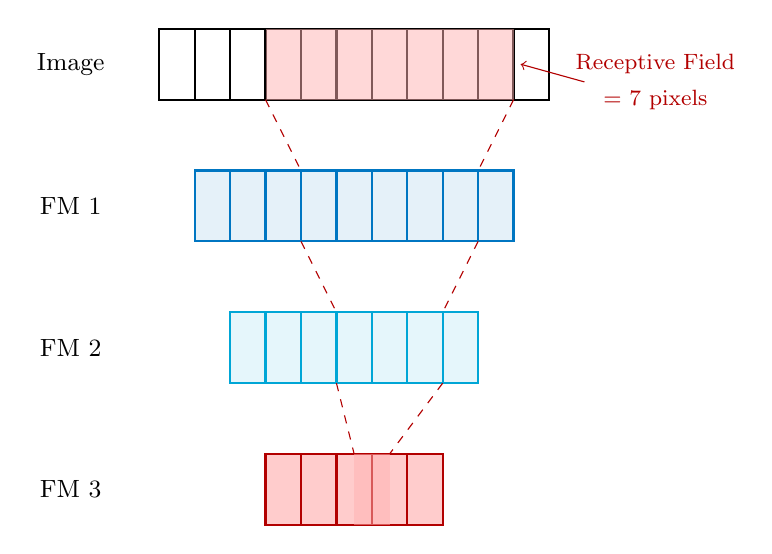
\begin{tikzpicture}[scale=0.45]
    % Layer labels
    \node[font=\small] at (-2.5, -2) {Image};
    \node[font=\small] at (-2.5, -6) {FM 1};
    \node[font=\small] at (-2.5, -10) {FM 2};
    \node[font=\small] at (-2.5, -14) {FM 3};
    
    % Image layer (11 units)
    \foreach \i in {0,...,10} {
        \draw[thick] (\i, -1) rectangle (\i+1, -3);
    }
    
    % Feature map 1 (9 units) - after 3x3 conv
    \foreach \i in {0,...,8} {
        \draw[thick, tudelftblue, fill=tudelftblue!10] (\i+1, -5) rectangle (\i+2, -7);
    }
    
    % Feature map 2 (7 units) - after 3x3 conv
    \foreach \i in {0,...,6} {
        \draw[thick, tudelftcyan, fill=tudelftcyan!10] (\i+2, -9) rectangle (\i+3, -11);
    }
    
    % Feature map 3 (5 units) - after 3x3 conv
    \foreach \i in {0,...,4} {
        \draw[thick, red!70!black, fill=red!20] (\i+3, -13) rectangle (\i+4, -15);
    }
    
    % Highlight receptive field
    \fill[red!30, opacity=0.5] (3, -1) rectangle (10, -3);
    \fill[red!30, opacity=0.5] (5.5, -13) rectangle (6.5, -15);
    
    % Connections showing receptive field growth
    \draw[dashed, red!70!black] (3, -3) -- (4, -5);
    \draw[dashed, red!70!black] (10, -3) -- (9, -5);
    \draw[dashed, red!70!black] (4, -7) -- (5, -9);
    \draw[dashed, red!70!black] (9, -7) -- (8, -9);
    \draw[dashed, red!70!black] (5, -11) -- (5.5, -13);
    \draw[dashed, red!70!black] (8, -11) -- (6.5, -13);
    
    % Annotation
    \node[font=\footnotesize, text=red!70!black] at (14, -2) {Receptive Field};
    \node[font=\footnotesize, text=red!70!black] at (14, -3) {= 7 pixels};
    \draw[->, red!70!black] (12, -2.5) -- (10.2, -2);
\end{tikzpicture}
\caption{Receptive field growth with stacked $3 \times 3$ convolutions. One unit in Feature Map 3 (highlighted) ``sees'' 7 pixels of the original image. Three $3 \times 3$ convs have the same receptive field as one $7 \times 7$ conv, but with far fewer parameters.}
\label{fig:receptive_field}
\end{figure}

\subsection{Convolution as a Sparse Matrix Multiplication}
Convolution can be viewed as multiplication by a sparse, structured \textbf{Toeplitz matrix}. For 1D convolution of $[x_1, x_2, x_3, x_4]$ with kernel $[-1, 0, 1]$:
\begin{equation}
\begin{bmatrix}
-1 & 0 & 1 & 0 \\
0 & -1 & 0 & 1 \\
\end{bmatrix}
\begin{bmatrix}
x_1 \\ x_2 \\ x_3 \\ x_4
\end{bmatrix}
=
\begin{bmatrix}
-x_1 + x_3 \\
-x_2 + x_4
\end{bmatrix}
\end{equation}
The matrix is:
\begin{itemize}
	\item \textbf{Sparse:} Many zeros, reducing computation.
	\item \textbf{Locally connected:} Non-zeros are clustered.
	\item \textbf{Weight-sharing:} The same kernel values appear in each row.
\end{itemize}
A CNN is a constrained fully-connected network. This constraint reduces parameters and encodes our prior knowledge about images.

\subsection{Residual Connections (ResNets)}
As networks become deeper (50, 100, 1000 layers), two problems arise:
\begin{enumerate}
	\item \textbf{Vanishing Gradients:} Gradients shrink exponentially as they backpropagate through many layers.
	\item \textbf{Degradation Problem:} Deeper networks often perform \textit{worse} than shallower ones on training data, even though they have more capacity.
\end{enumerate}

\textbf{Residual Networks (ResNets)} solve this with \textbf{skip connections}. Instead of learning a mapping $\mathcal{H}(\mathbf{x})$ directly, a residual block learns the \textbf{residual} $\mathcal{F}(\mathbf{x}) = \mathcal{H}(\mathbf{x}) - \mathbf{x}$:
\begin{equation}
	\mathbf{h}_{l+1} = \mathbf{h}_l + \mathcal{F}(\mathbf{h}_l; \mathbf{W}_l)
\end{equation}

\begin{figure}[H]
\centering
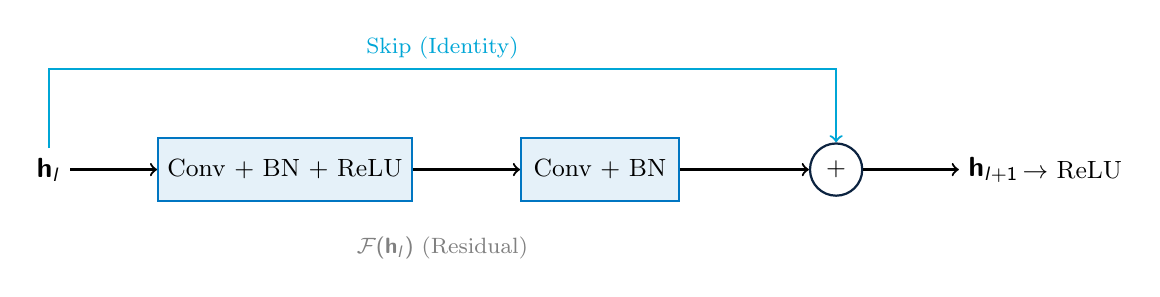
\begin{tikzpicture}[
    block/.style={rectangle, draw=tudelftblue, fill=tudelftblue!10, thick, minimum width=2cm, minimum height=0.8cm, font=\small},
    arrow/.style={->, thick},
    plus/.style={circle, draw=tudelftdarkblue, fill=white, thick, minimum size=0.5cm, font=\small}
]
    % Input
    \node (x) at (0, 0) {$\mathbf{h}_l$};
    
    % Conv blocks
    \node[block] (conv1) at (3, 0) {Conv + BN + ReLU};
    \node[block] (conv2) at (7, 0) {Conv + BN};
    
    % Plus
    \node[plus] (plus) at (10, 0) {$+$};
    
    % Output
    \node (out) at (12, 0) {$\mathbf{h}_{l+1}$};
    \node[font=\small] at (13, 0) {$\to$ ReLU};
    
    % Main path
    \draw[arrow] (x) -- (conv1);
    \draw[arrow] (conv1) -- (conv2);
    \draw[arrow] (conv2) -- (plus);
    \draw[arrow] (plus) -- (out);
    
    % Skip connection
    \draw[arrow, tudelftcyan, thick] (x.north) -- ++(0, 1) -| node[above, pos=0.25, font=\footnotesize, text=tudelftcyan] {Skip (Identity)} (plus.north);
    
    % Labels
    \node[font=\footnotesize, text=gray] at (5, -1) {$\mathcal{F}(\mathbf{h}_l)$ (Residual)};
\end{tikzpicture}
\caption{A Residual Block. The skip connection allows the input to bypass the weight layers. The block learns the residual $\mathcal{F}(\mathbf{h}_l)$, which is added to the input. If $\mathcal{F} = 0$, the block implements an identity mapping, which istrivially easy to learn.}
\label{fig:resnet_block}
\end{figure}

\paragraph{Why Skip Connections Work:}
\begin{itemize}
	\item \textbf{Gradient Highway:} During backpropagation, gradients can flow directly through the skip connection, bypassing the nonlinearities that cause vanishing gradients.
	\item \textbf{Easy Identity:} If the optimal solution is close to the identity, the network only needs to learn $\mathcal{F} \approx 0$, which is easier than learning a full identity mapping from scratch.
	\item \textbf{Ensemble Perspective:} A ResNet can be seen as an ensemble of many paths of varying depths, improving robustness.
\end{itemize}
ResNets enabled training of networks with 100+ layers and won the ImageNet 2015 competition by a large margin.


\section{Recurrent Neural Networks (RNNs)}
\label{sec:dl_rnn}

Feedforward networks and CNNs excel at processing fixed-size inputs, but many real-world problems involve \textbf{sequences} of variable length: text (words in a sentence), time series (stock prices), audio (speech frames), and more. For these tasks, we need architectures that can:
\begin{enumerate}
	\item Handle inputs of \textbf{arbitrary length}.
	\item Preserve the \textbf{order} of elements (``the cat sat on the mat'' $\neq$ ``mat the on sat cat the'').
	\item Model \textbf{long-range dependencies} (e.g., ``The student$_{[\text{singular}]}$, after reading the book, \textit{was}$_{[\text{singular}]}$ well prepared.'').
\end{enumerate}

\textbf{Recurrent Neural Networks (RNNs)} achieve this by maintaining an internal \textbf{hidden state} $\mathbf{h}_t$ that summarizes the sequence seen so far. At each time step, the network updates this state based on the current input and the previous state.

\subsection{The Recurrence Relation}
An RNN processes a sequence $\mathbf{x}_1, \mathbf{x}_2, \ldots, \mathbf{x}_T$ one element at a time. The core update rule is:
\begin{equation}
	\mathbf{h}_t = \phi(\mathbf{W}_{xh} \mathbf{x}_t + \mathbf{W}_{hh} \mathbf{h}_{t-1} + \mathbf{b}_h)
\end{equation}
where:
\begin{itemize}
	\item $\mathbf{h}_t \in \mathbb{R}^{d_h}$ is the hidden state at time $t$ (the ``memory'').
	\item $\mathbf{x}_t \in \mathbb{R}^{d_x}$ is the input at time $t$ (e.g., a one-hot encoded word).
	\item $\mathbf{W}_{xh} \in \mathbb{R}^{d_h \times d_x}$ transforms the input.
	\item $\mathbf{W}_{hh} \in \mathbb{R}^{d_h \times d_h}$ transforms the previous hidden state.
	\item $\phi$ is a non-linearity, typically $\tanh$ (outputs in $(-1, 1)$).
\end{itemize}
An optional output $\mathbf{y}_t$ can be computed from the hidden state: $\mathbf{y}_t = \mathbf{W}_{hy} \mathbf{h}_t + \mathbf{b}_y$.

\begin{figure}[H]
\centering
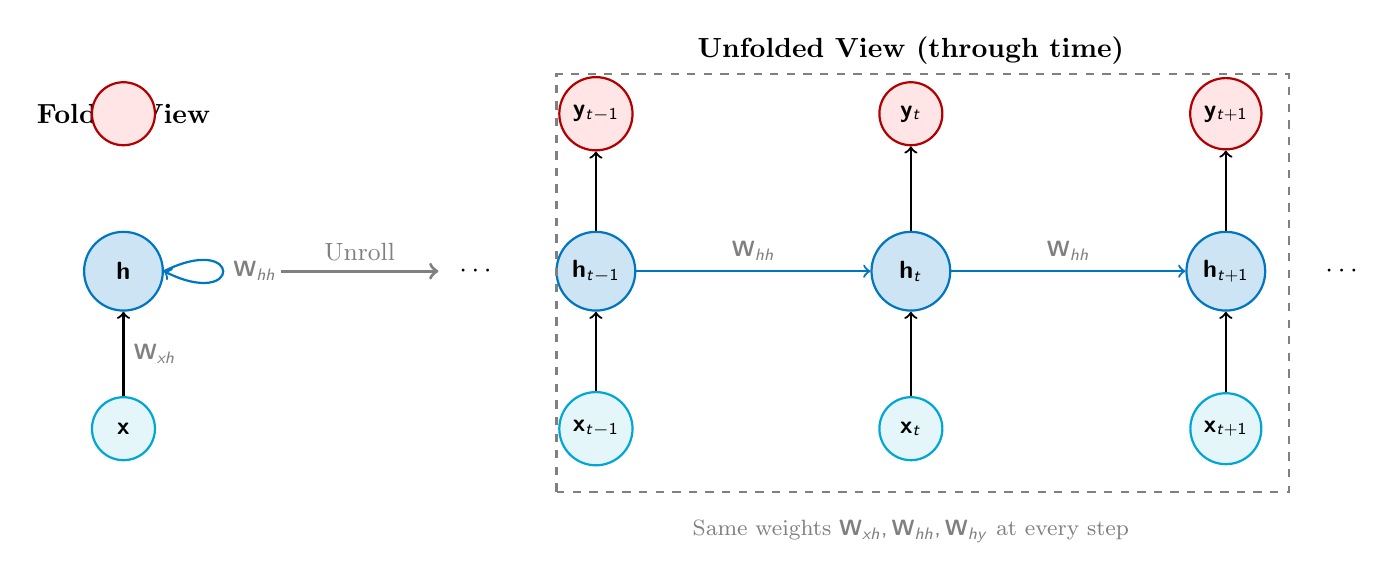
\begin{tikzpicture}[
    node distance=1.5cm,
    hidden/.style={circle, draw=tudelftblue, fill=tudelftblue!20, thick, minimum size=1cm, font=\small},
    input/.style={circle, draw=tudelftcyan, fill=tudelftcyan!10, thick, minimum size=0.8cm, font=\small},
    output/.style={circle, draw=red!70!black, fill=red!10, thick, minimum size=0.8cm, font=\small},
    arrow/.style={->, thick},
    weight/.style={font=\footnotesize, text=gray}
]
    % Folded representation (left)
    \node[font=\bfseries] at (-2, 2) {Folded View};
    \node[hidden] (h) at (-2, 0) {$\mathbf{h}$};
    \node[input] (x) at (-2, -2) {$\mathbf{x}$};
    \node[output] (y) at (-2, 2) {};
    \draw[arrow] (x) -- node[right, weight] {$\mathbf{W}_{xh}$} (h);
    \draw[arrow, tudelftblue, thick] (h.east) .. controls +(1, 0.5) and +(1, -0.5) .. node[right, weight] {$\mathbf{W}_{hh}$} (h.east);
    
    % Arrow between
    \draw[->, very thick, gray] (0, 0) -- (2, 0) node[midway, above, font=\small] {Unroll};
    
    % Unfolded representation (right)
    \node[font=\bfseries] at (8, 2.8) {Unfolded View (through time)};
    
    % Time step t-1
    \node[hidden] (h0) at (4, 0) {$\mathbf{h}_{t-1}$};
    \node[input] (x0) at (4, -2) {$\mathbf{x}_{t-1}$};
    \node[output] (y0) at (4, 2) {$\mathbf{y}_{t-1}$};
    \draw[arrow] (x0) -- (h0);
    \draw[arrow] (h0) -- (y0);
    
    % Time step t
    \node[hidden] (h1) at (8, 0) {$\mathbf{h}_t$};
    \node[input] (x1) at (8, -2) {$\mathbf{x}_t$};
    \node[output] (y1) at (8, 2) {$\mathbf{y}_t$};
    \draw[arrow] (x1) -- (h1);
    \draw[arrow] (h1) -- (y1);
    \draw[arrow, tudelftblue] (h0) -- node[above, weight] {$\mathbf{W}_{hh}$} (h1);
    
    % Time step t+1
    \node[hidden] (h2) at (12, 0) {$\mathbf{h}_{t+1}$};
    \node[input] (x2) at (12, -2) {$\mathbf{x}_{t+1}$};
    \node[output] (y2) at (12, 2) {$\mathbf{y}_{t+1}$};
    \draw[arrow] (x2) -- (h2);
    \draw[arrow] (h2) -- (y2);
    \draw[arrow, tudelftblue] (h1) -- node[above, weight] {$\mathbf{W}_{hh}$} (h2);
    
    % Dots
    \node at (2.5, 0) {$\cdots$};
    \node at (13.5, 0) {$\cdots$};
    
    % Shared weights annotation
    \draw[dashed, gray, thick] (3.5, -2.8) rectangle (12.8, 2.5);
    \node[font=\footnotesize, text=gray, align=center] at (8, -3.3) {Same weights $\mathbf{W}_{xh}, \mathbf{W}_{hh}, \mathbf{W}_{hy}$ at every step};
\end{tikzpicture}
\caption{\textbf{Left:} The folded (compact) view of an RNN, showing the self-loop on the hidden state. \textbf{Right:} The unfolded view, showing the network replicated across time steps. Crucially, all copies \textbf{share the same weights}, allowing the network to handle sequences of any length.}
\label{fig:rnn_unrolled}
\end{figure}

\paragraph{Key Insight: Parameter Sharing.}
Unlike a fully connected network where each position has separate weights, the RNN uses the \textbf{same} $\mathbf{W}_{xh}$ and $\mathbf{W}_{hh}$ at every time step. This:
\begin{itemize}
	\item Drastically reduces the number of parameters (independent of sequence length).
	\item Allows generalization to sequences longer than those seen during training.
	\item Encodes the prior that the ``rules'' of the sequence (e.g., grammar) are consistent across positions.
\end{itemize}

\subsection{Backpropagation Through Time (BPTT)}
To train an RNN, we \textbf{unroll} the network across all time steps and apply standard backpropagation on this unrolled graph. This is called \textbf{Backpropagation Through Time (BPTT)}.

Consider the gradient of the loss $L$ at time $T$ with respect to the hidden state at an earlier time $t$:
\begin{equation}
	\frac{\partial L_T}{\partial \mathbf{h}_t} = \frac{\partial L_T}{\partial \mathbf{h}_T} \cdot \prod_{k=t+1}^{T} \frac{\partial \mathbf{h}_k}{\partial \mathbf{h}_{k-1}}
\end{equation}
Each term $\frac{\partial \mathbf{h}_k}{\partial \mathbf{h}_{k-1}}$ is the Jacobian of the recurrence, which depends on $\mathbf{W}_{hh}$ and the derivative of $\tanh$. For long sequences, this becomes a product of $T - t$ matrices.

\subsection{The Vanishing and Exploding Gradient Problem}
The magnitude of gradients depends on the eigenvalues $\lambda$ of the effective weight matrix:
\begin{itemize}
	\item If $|\lambda| < 1$: The product of many terms $< 1$ shrinks exponentially $\to$ \textbf{Vanishing Gradients}. The network cannot learn long-range dependencies because gradients from distant past states are effectively zero.
	\item If $|\lambda| > 1$: The product grows exponentially $\to$ \textbf{Exploding Gradients}. Weights receive enormous updates, causing training to diverge (NaNs).
\end{itemize}

\begin{figure}[H]
\begin{pycode}
# Visualizing Vanishing and Exploding Gradients
T = 50
t_steps = np.arange(T)

# Simulate the effect of repeated multiplication w^t
w_vanish = 0.9
w_stable = 1.0
w_explode = 1.1

y_vanish = w_vanish ** t_steps
y_stable = w_stable ** t_steps
y_explode = w_explode ** t_steps

fig, ax = plt.subplots(figsize=(10, 5))

ax.plot(t_steps, y_vanish, '-', color=utils.COLORS['primary'], linewidth=2.5, label=r'Vanishing ($\lambda=0.9$)')
ax.plot(t_steps, y_stable, '--', color='gray', linewidth=2, label=r'Stable ($\lambda=1.0$)')
ax.plot(t_steps, y_explode, '-', color=utils.COLORS['red'], linewidth=2.5, label=r'Exploding ($\lambda=1.1$)')

ax.set_title(r'Effect of Repeated Multiplication ($\lambda^t$) Over Time')
ax.set_xlabel('Time Steps Back ($t$)')
ax.set_ylabel(r'Gradient Magnitude ($\lambda^t$)')
ax.legend()
ax.grid(True, linestyle=':', alpha=0.6)
ax.set_yscale('log')

utils.save_and_include("gradient_stability.pdf", width=r"0.9\textwidth")
\end{pycode}
\caption{The vanishing and exploding gradient problem. Even a small deviation from 1.0 in the eigenvalue leads to exponential decay or growth of gradient magnitude. Learning long-range dependencies becomes impossible because gradients from 50 steps ago are either $\approx 0$ or $\to \infty$.}
\label{fig:gradient_stability}
\end{figure}

\paragraph{Mitigation: Gradient Clipping.}
For exploding gradients, a simple fix is \textbf{gradient clipping}: if the norm of the gradient exceeds a threshold, rescale it:
\begin{equation}
	\mathbf{g} \leftarrow \min\left(1, \frac{\text{threshold}}{\|\mathbf{g}\|}\right) \cdot \mathbf{g}
\end{equation}
This prevents catastrophic updates but does not fix vanishing gradients.

\subsection{Gated Architectures: The Solution}
The fundamental problem is that vanilla RNNs transform the hidden state at every step, making it hard to preserve information unchanged. \textbf{Gated architectures} solve this by introducing \textbf{gates}, which are learned, data-dependent switches (values in $[0, 1]$) that control information flow.

The key idea: if a gate is ``open'' (value $\approx 1$), information (and gradients!) can flow through \textit{unchanged}. This creates a ``gradient highway'' that bypasses the vanishing gradient problem.

\subsubsection{Gated Recurrent Unit (GRU)}
The \textbf{GRU} uses two gates:

\begin{tcolorbox}[colback=tudelftblue!5!white, colframe=tudelftblue, title=GRU Equations]
\textbf{Reset Gate} (what to forget from the past):
\begin{equation}
	\mathbf{r}_t = \sigma(\mathbf{W}_{xr}\mathbf{x}_t + \mathbf{W}_{hr}\mathbf{h}_{t-1} + \mathbf{b}_r)
\end{equation}
\textbf{Update Gate} (how much of the past to keep):
\begin{equation}
	\mathbf{z}_t = \sigma(\mathbf{W}_{xz}\mathbf{x}_t + \mathbf{W}_{hz}\mathbf{h}_{t-1} + \mathbf{b}_z)
\end{equation}
\textbf{Candidate Hidden State} (new information):
\begin{equation}
	\tilde{\mathbf{h}}_t = \tanh(\mathbf{W}_{xh}\mathbf{x}_t + \mathbf{W}_{hh}(\mathbf{r}_t \odot \mathbf{h}_{t-1}) + \mathbf{b}_h)
\end{equation}
\textbf{Final Hidden State} (linear interpolation):
\begin{equation}
	\mathbf{h}_t = \mathbf{z}_t \odot \mathbf{h}_{t-1} + (1 - \mathbf{z}_t) \odot \tilde{\mathbf{h}}_t
\end{equation}
\end{tcolorbox}

\begin{itemize}
	\item If $\mathbf{z}_t \approx 1$: The new hidden state is almost the old one ($\mathbf{h}_t \approx \mathbf{h}_{t-1}$). Information is \textbf{preserved} across time, and gradients flow directly.
	\item If $\mathbf{z}_t \approx 0$: The new hidden state is the candidate ($\mathbf{h}_t \approx \tilde{\mathbf{h}}_t$). The memory is \textbf{reset} with new information.
	\item The reset gate $\mathbf{r}_t$ controls how much of $\mathbf{h}_{t-1}$ is used when computing the candidate.
\end{itemize}

\subsubsection{Long Short-Term Memory (LSTM)}
The \textbf{LSTM} is an older but still widely-used architecture. It introduces a separate \textbf{Cell State} $\mathbf{c}_t$ that acts as a ``conveyor belt'' for information, plus three gates:

\begin{tcolorbox}[colback=tudelftblue!5!white, colframe=tudelftblue, title=LSTM Equations]
\textbf{Forget Gate} (what to erase from cell):
\begin{equation}
	\mathbf{f}_t = \sigma(\mathbf{W}_{xf}\mathbf{x}_t + \mathbf{W}_{hf}\mathbf{h}_{t-1} + \mathbf{b}_f)
\end{equation}
\textbf{Input Gate} (what new information to write):
\begin{equation}
	\mathbf{i}_t = \sigma(\mathbf{W}_{xi}\mathbf{x}_t + \mathbf{W}_{hi}\mathbf{h}_{t-1} + \mathbf{b}_i)
\end{equation}
\textbf{Output Gate} (what to output from cell):
\begin{equation}
	\mathbf{o}_t = \sigma(\mathbf{W}_{xo}\mathbf{x}_t + \mathbf{W}_{ho}\mathbf{h}_{t-1} + \mathbf{b}_o)
\end{equation}
\textbf{Candidate Cell State}:
\begin{equation}
	\tilde{\mathbf{c}}_t = \tanh(\mathbf{W}_{xc}\mathbf{x}_t + \mathbf{W}_{hc}\mathbf{h}_{t-1} + \mathbf{b}_c)
\end{equation}
\textbf{Cell State Update} (linear combination):
\begin{equation}
	\mathbf{c}_t = \mathbf{f}_t \odot \mathbf{c}_{t-1} + \mathbf{i}_t \odot \tilde{\mathbf{c}}_t
\end{equation}
\textbf{Hidden State Output}:
\begin{equation}
	\mathbf{h}_t = \mathbf{o}_t \odot \tanh(\mathbf{c}_t)
\end{equation}
\end{tcolorbox}

\begin{figure}[H]
\centering
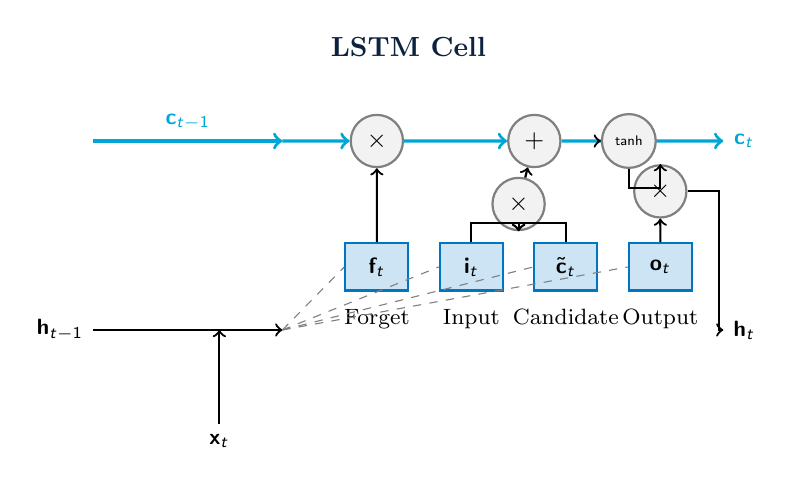
\begin{tikzpicture}[
    scale=0.8,
    gate/.style={rectangle, draw=tudelftblue, fill=tudelftblue!20, thick, minimum width=0.8cm, minimum height=0.6cm, font=\footnotesize},
    op/.style={circle, draw=gray, fill=gray!10, thick, minimum size=0.5cm, font=\small},
    cell/.style={rectangle, draw=tudelftcyan, fill=tudelftcyan!20, thick, rounded corners, minimum width=2cm, minimum height=0.6cm, font=\small},
    arrow/.style={->, thick},
    label/.style={font=\footnotesize}
]
    % Cell state conveyor belt
    \draw[arrow, tudelftcyan, very thick] (-3, 3) -- node[above, label] {$\mathbf{c}_{t-1}$} (0, 3);
    \node[op] (forget_mult) at (1.5, 3) {$\times$};
    \node[op] (add) at (4, 3) {$+$};
    \draw[arrow, tudelftcyan, very thick] (0, 3) -- (forget_mult);
    \draw[arrow, tudelftcyan, very thick] (forget_mult) -- (add);
    \draw[arrow, tudelftcyan, very thick] (add) -- (7, 3) node[right, label] {$\mathbf{c}_t$};
    
    % Forget gate
    \node[gate] (f) at (1.5, 1) {$\mathbf{f}_t$};
    \node[label, below=0.1cm of f] {Forget};
    \draw[arrow] (f) -- (forget_mult);
    
    % Input gate and candidate
    \node[gate] (i) at (3, 1) {$\mathbf{i}_t$};
    \node[label, below=0.1cm of i] {Input};
    \node[gate] (c_tilde) at (4.5, 1) {$\tilde{\mathbf{c}}_t$};
    \node[label, below=0.1cm of c_tilde] {Candidate};
    \node[op] (input_mult) at (3.75, 2) {$\times$};
    \draw[arrow] (i.north) -- ++(0, 0.3) -| (input_mult);
    \draw[arrow] (c_tilde.north) -- ++(0, 0.3) -| (input_mult);
    \draw[arrow] (input_mult) -- (add);
    
    % Output gate
    \node[gate] (o) at (6, 1) {$\mathbf{o}_t$};
    \node[label, below=0.1cm of o] {Output};
    \node[op] (tanh_out) at (5.5, 3) {\tiny$\tanh$};
    \node[op] (out_mult) at (6, 2.2) {$\times$};
    \draw[arrow] (5, 3) -- (tanh_out);
    \draw[arrow] (tanh_out.south) -- ++(0, -0.3) -| (out_mult.north);
    \draw[arrow] (o) -- (out_mult);
    
    % Hidden state
    \draw[arrow] (out_mult.east) -- ++(0.5, 0) |- (7, 0) node[right, label] {$\mathbf{h}_t$};
    
    % Inputs
    \draw[arrow] (-3, 0) node[left, label] {$\mathbf{h}_{t-1}$} -- (0, 0);
    \draw[arrow] (-1, -1.5) node[below, label] {$\mathbf{x}_t$} -- (-1, 0);
    
    % Connections to gates (conceptual)
    \draw[dashed, gray] (0, 0) -- (f.west);
    \draw[dashed, gray] (0, 0) -- (i.west);
    \draw[dashed, gray] (0, 0) -- (c_tilde.west);
    \draw[dashed, gray] (0, 0) -- (o.west);
    
    % Title
    \node[font=\bfseries, text=tudelftdarkblue] at (2, 4.5) {LSTM Cell};
\end{tikzpicture}
\caption{The LSTM architecture. The horizontal line at the top is the \textbf{Cell State} $\mathbf{c}_t$, a ``conveyor belt'' that can carry information unchanged across many time steps. Gates (forget, input, output) control what information is removed, added, or output at each step.}
\label{fig:lstm_cell}
\end{figure}

\paragraph{Why LSTMs Solve Vanishing Gradients:}
The cell state $\mathbf{c}_t$ is updated via \textbf{addition} (not multiplication):
\begin{equation}
	\mathbf{c}_t = \mathbf{f}_t \odot \mathbf{c}_{t-1} + \mathbf{i}_t \odot \tilde{\mathbf{c}}_t
\end{equation}
If $\mathbf{f}_t \approx 1$ and $\mathbf{i}_t \approx 0$, then $\mathbf{c}_t \approx \mathbf{c}_{t-1}$. The gradient $\frac{\partial \mathbf{c}_T}{\partial \mathbf{c}_t}$ involves products of forget gate values, not weight matrices. If forget gates are $\approx 1$, gradients flow through unchanged for hundreds of time steps.

\subsection{Summary: RNN Architectures}

\begin{table}[H]
\centering
\begin{tblr}{
  colspec = {l l l X[l]},
  row{1} = {font=\bfseries},
  hline{1,2,Z} = {solid},
}
Architecture & Gates & Cell State & Key Feature \\
Vanilla RNN & None & No & Simple but suffers from vanishing gradients \\
GRU & Reset, Update & No (merged with $\mathbf{h}$) & Simpler, fewer parameters than LSTM \\
LSTM & Forget, Input, Output & Yes ($\mathbf{c}_t$) & Gold standard, explicit memory cell \\
\end{tblr}
\caption{Comparison of RNN architectures. Gated architectures (GRU, LSTM) solve the vanishing gradient problem by allowing information to flow unchanged through time.}
\label{tab:rnn_architectures}
\end{table}


\section{Self-Attention and Transformers}
\label{sec:dl_transformers}

RNNs suffer from two fundamental limitations:
\begin{enumerate}
	\item \textbf{Sequential Processing:} Each hidden state depends on the previous one, preventing parallelization across time steps. Training is slow.
	\item \textbf{Vanishing Gradients:} Despite gating mechanisms, modeling very long-range dependencies remains challenging.
\end{enumerate}

The \textbf{Transformer} architecture (Vaswani et al., 2017, ``Attention Is All You Need'') revolutionized Deep Learning by discarding recurrence entirely. Instead, it uses \textbf{Self-Attention}, a mechanism where every token can directly attend to every other token in a single step, regardless of distance. This enables full parallelization and captures long-range dependencies effortlessly.

\subsection{The Core Idea: Weighted Aggregation}
Consider a sequence of word embeddings $\mathbf{x}_1, \mathbf{x}_2, \ldots, \mathbf{x}_n$. Self-attention produces new representations $\mathbf{y}_1, \ldots, \mathbf{y}_n$ where each $\mathbf{y}_i$ is a \textbf{weighted sum of all input embeddings}:
\begin{equation}
	\mathbf{y}_i = \sum_{j=1}^{n} w_{ij} \cdot \mathbf{x}_j
\end{equation}
The key question is: how do we determine the weights $w_{ij}$?

\paragraph{Step 1: Compute Similarity.}
We measure how ``relevant'' token $j$ is to token $i$ using a dot product (similarity):
\begin{equation}
	e_{ij} = \mathbf{x}_i^\top \mathbf{x}_j
\end{equation}

\paragraph{Step 2: Normalize with Softmax.}
The raw scores $e_{ij}$ can be any real number. We convert them to proper probability-like weights using softmax:
\begin{equation}
	w_{ij} = \frac{\exp(e_{ij})}{\sum_{k=1}^{n} \exp(e_{ik})}
\end{equation}
This ensures $\sum_j w_{ij} = 1$ and $w_{ij} \geq 0$ for all $j$.

\paragraph{Step 3: Weighted Aggregation.}
Each output $\mathbf{y}_i$ is a convex combination of all input vectors, with weights determined by their similarity to $\mathbf{x}_i$.

\subsection{Queries, Keys, and Values}
The basic attention formula uses the same embedding $\mathbf{x}$ for two different purposes:
\begin{enumerate}
	\item \textbf{Determining relevance} (computing $e_{ij}$).
	\item \textbf{Providing content} (being aggregated into $\mathbf{y}_i$).
\end{enumerate}
These are conceptually different tasks. Consider:
\begin{quote}
	``The \textit{student}, after reading the book, \textit{was} prepared.''
\end{quote}
When deciding how ``student'' influences ``was'', we care about grammatical features (singular noun $\to$ singular verb). But when aggregating content from ``student'' into ``was'', we might want semantic features (the concept of a person).

The Transformer introduces three \textbf{learned linear projections} for each embedding:
\begin{tcolorbox}[colback=tudelftblue!5!white, colframe=tudelftblue, 
    title={Query $\mid$ Key $\mid$ Value}]
For each input embedding $\mathbf{x}_i$:
\begin{align}
	\mathbf{q}_i &= \mathbf{W}_Q \mathbf{x}_i \quad \text{(Query: ``What am I looking for?'')} \\
	\mathbf{k}_i &= \mathbf{W}_K \mathbf{x}_i \quad \text{(Key: ``What do I contain?'')} \\
	\mathbf{v}_i &= \mathbf{W}_V \mathbf{x}_i \quad \text{(Value: ``What should I contribute?'')}
\end{align}
The attention weight from $i$ to $j$ is computed using queries and keys:
\begin{equation}
	e_{ij} = \mathbf{q}_i^\top \mathbf{k}_j
\end{equation}
The output uses values:
\begin{equation}
	\mathbf{y}_i = \sum_{j=1}^{n} w_{ij} \cdot \mathbf{v}_j
\end{equation}
\end{tcolorbox}

The intuition:
\begin{itemize}
	\item A \textbf{verb} (``was'') emits a query looking for its subject's number (singular/plural).
	\item A \textbf{noun} (``student'') advertises via its key that it is a singular noun.
	\item The dot product $\mathbf{q}_{\text{was}}^\top \mathbf{k}_{\text{student}}$ is high $\to$ high attention weight.
	\item ``student'''s \textbf{value} (perhaps encoding ``singular'') is then added to ``was'''s representation.
\end{itemize}

\begin{figure}[H]
\centering
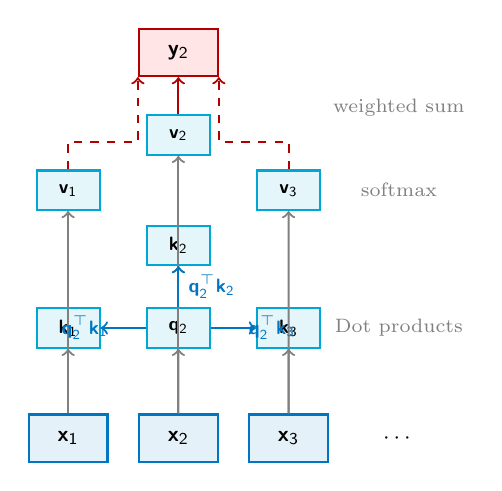
\begin{tikzpicture}[
    scale=0.7,
    embed/.style={rectangle, draw=tudelftblue, fill=tudelftblue!10, thick, minimum width=1cm, minimum height=0.6cm, font=\footnotesize},
    proj/.style={rectangle, draw=tudelftcyan, fill=tudelftcyan!10, thick, minimum width=0.8cm, minimum height=0.5cm, font=\scriptsize},
    score/.style={rectangle, draw=gray, fill=gray!10, thick, minimum width=0.6cm, minimum height=0.6cm, font=\scriptsize},
    output/.style={rectangle, draw=red!70!black, fill=red!10, thick, minimum width=1cm, minimum height=0.6cm, font=\footnotesize},
    arrow/.style={->, thick}
]
    % Input embeddings
    \node[embed] (x1) at (0, 0) {$\mathbf{x}_1$};
    \node[embed] (x2) at (2, 0) {$\mathbf{x}_2$};
    \node[embed] (x3) at (4, 0) {$\mathbf{x}_3$};
    \node[font=\footnotesize] at (6, 0) {$\cdots$};
    
    % Q, K, V projections for x2
    \node[proj] (q2) at (2, 2) {$\mathbf{q}_2$};
    \node[proj] (k1) at (0, 2) {$\mathbf{k}_1$};
    \node[proj] (k2) at (2, 3.5) {$\mathbf{k}_2$};
    \node[proj] (k3) at (4, 2) {$\mathbf{k}_3$};
    \node[proj] (v1) at (0, 4.5) {$\mathbf{v}_1$};
    \node[proj] (v2) at (2, 5.5) {$\mathbf{v}_2$};
    \node[proj] (v3) at (4, 4.5) {$\mathbf{v}_3$};
    
    % Arrows from inputs to projections
    \draw[arrow, gray] (x1) -- (k1);
    \draw[arrow, gray] (x2) -- (q2);
    \draw[arrow, gray] (x2) -- (k2);
    \draw[arrow, gray] (x3) -- (k3);
    \draw[arrow, gray] (x1) -- (v1);
    \draw[arrow, gray] (x2) -- (v2);
    \draw[arrow, gray] (x3) -- (v3);
    
    % Dot products (scores)
    \draw[arrow, tudelftblue] (q2.west) -- +(-0.5, 0) |- node[left, font=\scriptsize] {$\mathbf{q}_2^\top \mathbf{k}_1$} (k1.east);
    \draw[arrow, tudelftblue] (q2.north) -- node[right, font=\scriptsize] {$\mathbf{q}_2^\top \mathbf{k}_2$} (k2.south);
    \draw[arrow, tudelftblue] (q2.east) -- +(0.5, 0) |- node[right, font=\scriptsize] {$\mathbf{q}_2^\top \mathbf{k}_3$} (k3.west);
    
    % Output
    \node[output] (y2) at (2, 7) {$\mathbf{y}_2$};
    
    % Weighted sum arrows
    \draw[arrow, red!70!black, dashed] (v1.north) -- ++(0, 0.5) -| (y2.south west);
    \draw[arrow, red!70!black] (v2.north) -- (y2.south);
    \draw[arrow, red!70!black, dashed] (v3.north) -- ++(0, 0.5) -| (y2.south east);
    
    % Annotations
    \node[font=\scriptsize, text=gray] at (6, 2) {Dot products};
    \node[font=\scriptsize, text=gray] at (6, 4.5) {softmax};
    \node[font=\scriptsize, text=gray] at (6, 6) {weighted sum};
\end{tikzpicture}
\caption{Self-Attention for computing $\mathbf{y}_2$. The query $\mathbf{q}_2$ is compared to all keys via dot product. After softmax, the resulting weights multiply the values, which are summed to produce the output.}
\label{fig:self_attention_mechanism}
\end{figure}

\subsection{Scaled Dot-Product Attention}
In matrix form, for a sequence of $n$ tokens with embedding dimension $d$:
\begin{equation}
	\mathbf{Q} = \mathbf{X}\mathbf{W}_Q, \quad \mathbf{K} = \mathbf{X}\mathbf{W}_K, \quad \mathbf{V} = \mathbf{X}\mathbf{W}_V
\end{equation}
where $\mathbf{X} \in \mathbb{R}^{n \times d}$ and $\mathbf{W}_Q, \mathbf{W}_K, \mathbf{W}_V \in \mathbb{R}^{d \times d_k}$.

The full attention formula is:
\begin{equation}
	\text{Attention}(\mathbf{Q}, \mathbf{K}, \mathbf{V}) = \text{softmax}\left( \frac{\mathbf{Q}\mathbf{K}^\top}{\sqrt{d_k}} \right) \mathbf{V}
\end{equation}

\paragraph{Why scale by $\sqrt{d_k}$?}
The dot product $\mathbf{q}^\top \mathbf{k}$ has variance proportional to $d_k$ (each element of $\mathbf{q}$ and $\mathbf{k}$ contributes to the sum). For large $d_k$, some dot products become very large, pushing softmax into saturation (outputs close to 0 or 1) where gradients are tiny. Dividing by $\sqrt{d_k}$ normalizes the variance to $\approx 1$, keeping softmax in a well-behaved regime.

\subsection{Multi-Head Attention}
A single attention head learns one type of relationship (e.g., subject-verb agreement). But language has many simultaneous relationships (grammar, coreference, semantic roles). \textbf{Multi-Head Attention} runs $h$ attention heads in parallel, each with its own $\mathbf{W}_Q^{(r)}, \mathbf{W}_K^{(r)}, \mathbf{W}_V^{(r)}$:
\begin{equation}
	\text{head}_r = \text{Attention}(\mathbf{Q}^{(r)}, \mathbf{K}^{(r)}, \mathbf{V}^{(r)})
\end{equation}
The outputs are concatenated and projected:
\begin{equation}
	\text{MultiHead}(\mathbf{Q}, \mathbf{K}, \mathbf{V}) = \text{Concat}(\text{head}_1, \ldots, \text{head}_h) \mathbf{W}^O
\end{equation}
Typically, if the model dimension is $d = 512$ and we use $h = 8$ heads, each head operates on $d_k = d/h = 64$ dimensions.

\begin{figure}[H]
\centering
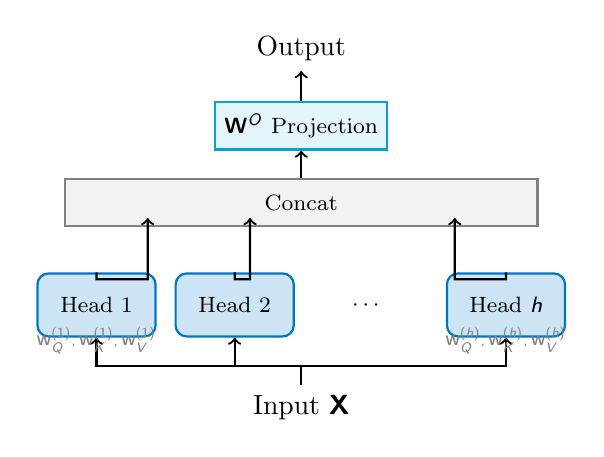
\begin{tikzpicture}[
    scale=0.65,
    head/.style={rectangle, draw=tudelftblue, fill=tudelftblue!20, thick, rounded corners, minimum width=1.5cm, minimum height=0.8cm, font=\footnotesize},
    proj/.style={rectangle, draw=tudelftcyan, fill=tudelftcyan!10, thick, minimum width=1.5cm, minimum height=0.6cm, font=\footnotesize},
    concat/.style={rectangle, draw=gray, fill=gray!10, thick, minimum width=6cm, minimum height=0.6cm, font=\footnotesize},
    arrow/.style={->, thick}
]
    % Input
    \node (input) at (0, 0) {Input $\mathbf{X}$};
    
    % Heads
    \node[head] (h1) at (-4, 2) {Head 1};
    \node[head] (h2) at (-1.3, 2) {Head 2};
    \node[font=\footnotesize] at (1.3, 2) {$\cdots$};
    \node[head] (hh) at (4, 2) {Head $h$};
    
    % Arrows to heads
    \draw[arrow] (input) -- ++(0, 0.8) -| (h1);
    \draw[arrow] (input) -- ++(0, 0.8) -| (h2);
    \draw[arrow] (input) -- ++(0, 0.8) -| (hh);
    
    % Concat
    \node[concat] (concat) at (0, 4) {Concat};
    
    \draw[arrow] (h1) -- ++(0, 0.5) -| (-3, 3.7);
    \draw[arrow] (h2) -- ++(0, 0.5) -| (-1, 3.7);
    \draw[arrow] (hh) -- ++(0, 0.5) -| (3, 3.7);
    
    % Output projection
    \node[proj] (wo) at (0, 5.5) {$\mathbf{W}^O$ Projection};
    \draw[arrow] (concat) -- (wo);
    
    % Output
    \node (output) at (0, 7) {Output};
    \draw[arrow] (wo) -- (output);
    
    % Annotations inside heads
    \node[font=\tiny, text=gray] at (-4, 1.3) {$\mathbf{W}_Q^{(1)}, \mathbf{W}_K^{(1)}, \mathbf{W}_V^{(1)}$};
    \node[font=\tiny, text=gray] at (4, 1.3) {$\mathbf{W}_Q^{(h)}, \mathbf{W}_K^{(h)}, \mathbf{W}_V^{(h)}$};
\end{tikzpicture}
\caption{Multi-Head Attention. Each head has its own Q, K, V projections and computes attention independently. Outputs are concatenated and projected back to the model dimension.}
\label{fig:multi_head_attention}
\end{figure}

\subsection{Positional Encodings}
The self-attention formula is \textbf{permutation invariant}: if we shuffle the input tokens, the outputs are shuffled the same way, but the attention weights themselves don't change. The model has no notion of word order!

To inject position information, we add \textbf{Positional Encodings} to the input embeddings:
\begin{equation}
	\mathbf{x}_t' = \mathbf{x}_t + \mathbf{p}_t
\end{equation}
The original Transformer uses fixed sinusoidal encodings:
\begin{align}
	\text{PE}_{(pos, 2i)} &= \sin\left(\frac{pos}{10000^{2i/d}}\right) \\
	\text{PE}_{(pos, 2i+1)} &= \cos\left(\frac{pos}{10000^{2i/d}}\right)
\end{align}
where $pos$ is the position and $i$ is the dimension index. Different frequencies allow the model to learn to attend to relative positions.

Modern models often use \textbf{learned positional embeddings} or more advanced schemes like Rotary Position Embedding (RoPE).

\subsection{The Transformer Block}
A complete Transformer layer combines Multi-Head Attention with a Feed-Forward Network (FFN), using residual connections and layer normalization:

\begin{figure}[H]
\centering
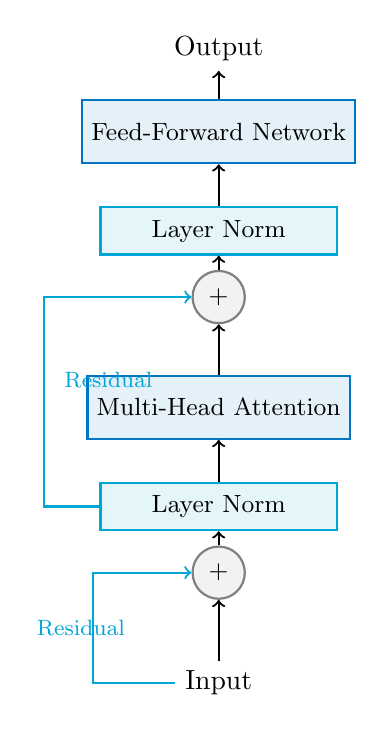
\begin{tikzpicture}[
    scale=0.7,
    block/.style={rectangle, draw=tudelftblue, fill=tudelftblue!10, thick, minimum width=3cm, minimum height=0.8cm, font=\small},
    norm/.style={rectangle, draw=tudelftcyan, fill=tudelftcyan!10, thick, minimum width=3cm, minimum height=0.6cm, font=\small},
    add/.style={circle, draw=gray, fill=gray!10, thick, minimum size=0.5cm, font=\small},
    arrow/.style={->, thick}
]
    % Input
    \node (input) at (0, 0) {Input};
    
    % Add + Norm 1
    \node[add] (add1) at (0, 2) {$+$};
    \node[norm] (norm1) at (0, 3.2) {Layer Norm};
    
    % Multi-Head Attention
    \node[block] (mha) at (0, 5) {Multi-Head Attention};
    
    % Add + Norm 2
    \node[add] (add2) at (0, 7) {$+$};
    \node[norm] (norm2) at (0, 8.2) {Layer Norm};
    
    % FFN
    \node[block] (ffn) at (0, 10) {Feed-Forward Network};
    
    % Output
    \node (output) at (0, 11.5) {Output};
    
    % Main path
    \draw[arrow] (input) -- (add1);
    \draw[arrow] (add1) -- (norm1);
    \draw[arrow] (norm1) -- (mha);
    \draw[arrow] (mha) -- (add2);
    \draw[arrow] (add2) -- (norm2);
    \draw[arrow] (norm2) -- (ffn);
    \draw[arrow] (ffn) -- (output);
    
    % Residual connections
    \draw[arrow, tudelftcyan] (input.west) -- ++(-1.5, 0) |- (add1.west);
    \draw[arrow, tudelftcyan] (norm1.west) -- ++(-1, 0) |- (add2.west);
    
    % Labels
    \node[font=\footnotesize, text=tudelftcyan] at (-2.5, 1) {Residual};
    \node[font=\footnotesize, text=tudelftcyan] at (-2, 5.5) {Residual};
\end{tikzpicture}
\caption{A Transformer Block (Post-Norm variant). Multi-Head Attention is followed by a Feed-Forward Network. Residual connections (skip connections) and Layer Normalization are applied after each sub-layer, enabling stable training of very deep models.}
\label{fig:transformer_block}
\end{figure}

The Feed-Forward Network is a simple two-layer MLP applied position-wise:
\begin{equation}
	\text{FFN}(\mathbf{x}) = \max(0, \mathbf{x}\mathbf{W}_1 + \mathbf{b}_1)\mathbf{W}_2 + \mathbf{b}_2
\end{equation}
It expands the dimension (e.g., $512 \to 2048$), applies a non-linearity, and projects back.

\subsection{Why Transformers Dominate}
\begin{itemize}
	\item \textbf{Parallelization:} All attention computations for all positions happen simultaneously. Training is highly efficient on modern GPUs.
	\item \textbf{Long-Range Dependencies:} Any two tokens interact directly in a single attention layer, regardless of distance.
	\item \textbf{Scalability:} The architecture scales to billions of parameters and trillions of tokens (foundation models like GPT, BERT, LLaMA).
	\item \textbf{Flexibility:} The same architecture works for language, vision (ViT), audio, and multimodal tasks.
\end{itemize}

\begin{figure}[H]
\centering
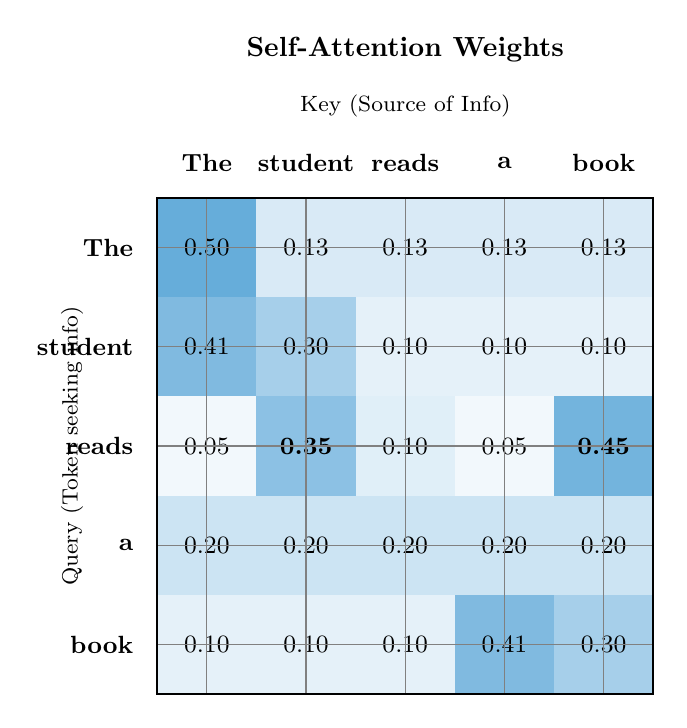
\begin{tikzpicture}[
    scale=0.9,
    cell/.style={minimum width=1.4cm, minimum height=1.4cm, font=\small},
    label/.style={font=\small\bfseries}
]
    % Define attention weights (pre-computed from softmax)
    % Row = Query, Col = Key
    % Row 0: "The" -> weights [0.50, 0.13, 0.13, 0.13, 0.13]
    % Row 1: "student" -> weights [0.41, 0.30, 0.10, 0.10, 0.10]
    % Row 2: "reads" -> weights [0.05, 0.35, 0.10, 0.05, 0.45]
    % Row 3: "a" -> weights [0.20, 0.20, 0.20, 0.20, 0.20]
    % Row 4: "book" -> weights [0.10, 0.10, 0.10, 0.41, 0.30]
    
    % Column labels (Keys)
    \node[label] at (1.4, 1.2) {The};
    \node[label] at (2.8, 1.2) {student};
    \node[label] at (4.2, 1.2) {reads};
    \node[label] at (5.6, 1.2) {a};
    \node[label] at (7.0, 1.2) {book};
    
    % Row labels (Queries)
    \node[label, anchor=east] at (0.5, 0) {The};
    \node[label, anchor=east] at (0.5, -1.4) {student};
    \node[label, anchor=east] at (0.5, -2.8) {reads};
    \node[label, anchor=east] at (0.5, -4.2) {a};
    \node[label, anchor=east] at (0.5, -5.6) {book};
    
    % Row 0: The
    \fill[tudelftblue!60] (0.7, -0.7) rectangle (2.1, 0.7);
    \fill[tudelftblue!15] (2.1, -0.7) rectangle (3.5, 0.7);
    \fill[tudelftblue!15] (3.5, -0.7) rectangle (4.9, 0.7);
    \fill[tudelftblue!15] (4.9, -0.7) rectangle (6.3, 0.7);
    \fill[tudelftblue!15] (6.3, -0.7) rectangle (7.7, 0.7);
    \node[cell] at (1.4, 0) {0.50};
    \node[cell] at (2.8, 0) {0.13};
    \node[cell] at (4.2, 0) {0.13};
    \node[cell] at (5.6, 0) {0.13};
    \node[cell] at (7.0, 0) {0.13};
    
    % Row 1: student
    \fill[tudelftblue!50] (0.7, -2.1) rectangle (2.1, -0.7);
    \fill[tudelftblue!35] (2.1, -2.1) rectangle (3.5, -0.7);
    \fill[tudelftblue!10] (3.5, -2.1) rectangle (4.9, -0.7);
    \fill[tudelftblue!10] (4.9, -2.1) rectangle (6.3, -0.7);
    \fill[tudelftblue!10] (6.3, -2.1) rectangle (7.7, -0.7);
    \node[cell] at (1.4, -1.4) {0.41};
    \node[cell] at (2.8, -1.4) {0.30};
    \node[cell] at (4.2, -1.4) {0.10};
    \node[cell] at (5.6, -1.4) {0.10};
    \node[cell] at (7.0, -1.4) {0.10};
    
    % Row 2: reads (high attention to student and book)
    \fill[tudelftblue!5] (0.7, -3.5) rectangle (2.1, -2.1);
    \fill[tudelftblue!45] (2.1, -3.5) rectangle (3.5, -2.1);
    \fill[tudelftblue!12] (3.5, -3.5) rectangle (4.9, -2.1);
    \fill[tudelftblue!5] (4.9, -3.5) rectangle (6.3, -2.1);
    \fill[tudelftblue!55] (6.3, -3.5) rectangle (7.7, -2.1);
    \node[cell] at (1.4, -2.8) {0.05};
    \node[cell] at (2.8, -2.8) {\textbf{0.35}};
    \node[cell] at (4.2, -2.8) {0.10};
    \node[cell] at (5.6, -2.8) {0.05};
    \node[cell] at (7.0, -2.8) {\textbf{0.45}};
    
    % Row 3: a
    \fill[tudelftblue!20] (0.7, -4.9) rectangle (2.1, -3.5);
    \fill[tudelftblue!20] (2.1, -4.9) rectangle (3.5, -3.5);
    \fill[tudelftblue!20] (3.5, -4.9) rectangle (4.9, -3.5);
    \fill[tudelftblue!20] (4.9, -4.9) rectangle (6.3, -3.5);
    \fill[tudelftblue!20] (6.3, -4.9) rectangle (7.7, -3.5);
    \node[cell] at (1.4, -4.2) {0.20};
    \node[cell] at (2.8, -4.2) {0.20};
    \node[cell] at (4.2, -4.2) {0.20};
    \node[cell] at (5.6, -4.2) {0.20};
    \node[cell] at (7.0, -4.2) {0.20};
    
    % Row 4: book (high attention to a)
    \fill[tudelftblue!10] (0.7, -6.3) rectangle (2.1, -4.9);
    \fill[tudelftblue!10] (2.1, -6.3) rectangle (3.5, -4.9);
    \fill[tudelftblue!10] (3.5, -6.3) rectangle (4.9, -4.9);
    \fill[tudelftblue!50] (4.9, -6.3) rectangle (6.3, -4.9);
    \fill[tudelftblue!35] (6.3, -6.3) rectangle (7.7, -4.9);
    \node[cell] at (1.4, -5.6) {0.10};
    \node[cell] at (2.8, -5.6) {0.10};
    \node[cell] at (4.2, -5.6) {0.10};
    \node[cell] at (5.6, -5.6) {0.41};
    \node[cell] at (7.0, -5.6) {0.30};
    
    % Grid lines
    \draw[gray] (0.7, 0.7) grid[step=1.4] (7.7, -6.3);
    \draw[thick] (0.7, 0.7) rectangle (7.7, -6.3);
    
    % Axis labels
    \node[font=\footnotesize, rotate=90] at (-0.5, -2.8) {Query (Token seeking info)};
    \node[font=\footnotesize] at (4.2, 2) {Key (Source of Info)};
    
    % Title
    \node[font=\bfseries] at (4.2, 2.8) {Self-Attention Weights};
\end{tikzpicture}
\caption{Heatmap of Attention Weights for ``The student reads a book.'' The verb ``reads'' (Query) assigns high attention to its subject ``student'' and object ``book'' (Keys), aggregating their information. Darker cells indicate higher attention weights.}
\label{fig:attention_heatmap}
\end{figure}


\section{Unsupervised Learning and Generative Models}
\label{sec:dl_unsupervised}

In Supervised Learning, we have labeled examples $(\mathbf{x}, \mathbf{y})$ and learn a mapping $\mathbf{x} \to \mathbf{y}$. In \textbf{Unsupervised Learning}, we only have data $\mathbf{x}$ with no labels. The goal is to discover the underlying \textbf{structure} of the data distribution $p_{\text{data}}(\mathbf{x})$.

\paragraph{Why Unsupervised Learning?}
\begin{itemize}
	\item \textbf{Labels are expensive:} Annotating millions of images or documents requires significant human effort.
	\item \textbf{Compression:} Learning compact representations for efficient storage and transmission.
	\item \textbf{Feature learning:} Pre-training representations that transfer to downstream tasks.
	\item \textbf{Generation:} Creating new synthetic data (images, text, audio) that looks like the training data.
\end{itemize}

\subsection{Autoencoders}
An \textbf{Autoencoder} learns to compress data into a lower-dimensional representation and then reconstruct it. It consists of two parts:
\begin{itemize}
	\item \textbf{Encoder} $f$: Maps input $\mathbf{x}$ to a latent code $\mathbf{h} = f(\mathbf{x})$.
	\item \textbf{Decoder} $g$: Reconstructs the input from the code $\hat{\mathbf{x}} = g(\mathbf{h})$.
\end{itemize}
The training objective is to minimize reconstruction error:
\begin{equation}
	\mathcal{L} = \|\mathbf{x} - g(f(\mathbf{x}))\|^2
\end{equation}

\begin{figure}[H]
\centering
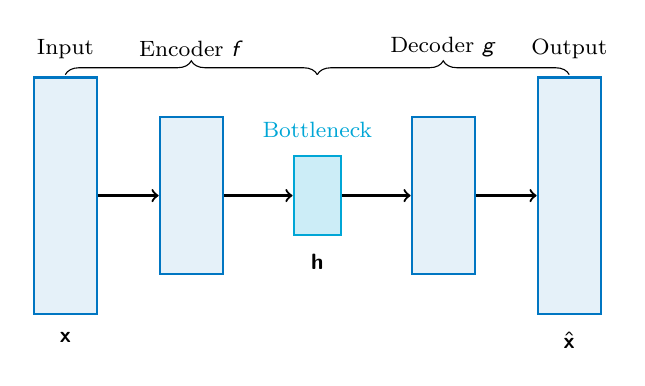
\begin{tikzpicture}[
    scale=0.8,
    layer/.style={rectangle, draw=tudelftblue, fill=tudelftblue!10, thick, minimum width=0.8cm, font=\footnotesize},
    latent/.style={rectangle, draw=tudelftcyan, fill=tudelftcyan!20, thick, minimum width=0.6cm, font=\footnotesize},
    arrow/.style={->, thick}
]
    % Input
    \node[layer, minimum height=3cm] (input) at (0, 0) {};
    \node[below=0.1cm of input, font=\footnotesize] {$\mathbf{x}$};
    \node[above=0.1cm of input, font=\footnotesize] {Input};
    
    % Encoder hidden
    \node[layer, minimum height=2cm] (enc1) at (2, 0) {};
    
    % Latent (bottleneck)
    \node[latent, minimum height=1cm] (latent) at (4, 0) {};
    \node[below=0.1cm of latent, font=\footnotesize] {$\mathbf{h}$};
    \node[above=0.1cm of latent, font=\footnotesize, text=tudelftcyan] {Bottleneck};
    
    % Decoder hidden
    \node[layer, minimum height=2cm] (dec1) at (6, 0) {};
    
    % Output
    \node[layer, minimum height=3cm] (output) at (8, 0) {};
    \node[below=0.1cm of output, font=\footnotesize] {$\hat{\mathbf{x}}$};
    \node[above=0.1cm of output, font=\footnotesize] {Output};
    
    % Arrows
    \draw[arrow] (input) -- (enc1);
    \draw[arrow] (enc1) -- (latent);
    \draw[arrow] (latent) -- (dec1);
    \draw[arrow] (dec1) -- (output);
    
    % Labels
    \draw[decorate, decoration={brace, amplitude=5pt, raise=5pt}] (0, 1.7) -- (4, 1.7) node[midway, above=8pt, font=\footnotesize] {Encoder $f$};
    \draw[decorate, decoration={brace, amplitude=5pt, raise=5pt}] (4, 1.7) -- (8, 1.7) node[midway, above=8pt, font=\footnotesize] {Decoder $g$};
\end{tikzpicture}
\caption{Autoencoder architecture. The encoder compresses the input through progressively smaller layers until reaching the \textbf{bottleneck} (latent code $\mathbf{h}$). The decoder then expands it back to reconstruct the input.}
\label{fig:autoencoder}
\end{figure}

\paragraph{Undercomplete vs. Overcomplete:}
\begin{itemize}
	\item \textbf{Undercomplete} ($\dim(\mathbf{h}) < \dim(\mathbf{x})$): The bottleneck forces compression. The network must learn the most important features to reconstruct $\mathbf{x}$ from $\mathbf{h}$. Similar to PCA but with non-linear mappings.
	\item \textbf{Overcomplete} ($\dim(\mathbf{h}) \geq \dim(\mathbf{x})$): No compression needed, the network could simply copy the input. We need regularization to learn useful features.
\end{itemize}

\paragraph{Denoising Autoencoders (DAEs):}
A powerful regularization strategy is to train the autoencoder to \textbf{denoise} corrupted inputs:
\begin{equation}
	\mathcal{L}_{\text{DAE}} = \|\mathbf{x} - g(f(\tilde{\mathbf{x}}))\|^2, \quad \tilde{\mathbf{x}} = \mathbf{x} + \epsilon, \quad \epsilon \sim \mathcal{N}(0, \sigma^2)
\end{equation}
The network receives a noisy version $\tilde{\mathbf{x}}$ but must output the clean $\mathbf{x}$. This forces it to learn the \textbf{data manifold},the low-dimensional structure underlying high-dimensional data.

\subsection{Generative Models: The Core Idea}
Generative models aim to \textbf{sample new data} from $p_{\text{data}}(\mathbf{x})$. Since this distribution is complex and unknown, we can't sample directly. The key insight:
\begin{center}
	\textit{Transform samples from a simple distribution (e.g., $\mathbf{z} \sim \mathcal{N}(0, \mathbf{I})$) into the complex data distribution.}
\end{center}
All major generative models (VAE, GAN, Diffusion) follow this principle but differ in how they learn the transformation.

\subsection{Variational Autoencoders (VAEs)}
A standard autoencoder maps each input to a single point in latent space. This makes generation difficult, because we don't know what points in latent space correspond to valid data. \textbf{VAEs} solve this by making the latent space probabilistic.

\begin{tcolorbox}[colback=tudelftblue!5!white, colframe=tudelftblue, title=VAE Architecture]
\textbf{Encoder:} Maps $\mathbf{x}$ to the \textit{parameters} of a distribution, not a single point:
\begin{equation}
	q_\phi(\mathbf{z} | \mathbf{x}) = \mathcal{N}(\boldsymbol{\mu}_\phi(\mathbf{x}), \boldsymbol{\sigma}_\phi^2(\mathbf{x}))
\end{equation}
\textbf{Decoder:} Samples $\mathbf{z}$ from this distribution and reconstructs:
\begin{equation}
	p_\theta(\mathbf{x} | \mathbf{z})
\end{equation}
\end{tcolorbox}

\paragraph{The Reparameterization Trick:}
We can't backpropagate through random sampling. The trick: express the randomness \textit{externally}:
\begin{equation}
	\mathbf{z} = \boldsymbol{\mu} + \boldsymbol{\sigma} \odot \boldsymbol{\epsilon}, \quad \boldsymbol{\epsilon} \sim \mathcal{N}(0, \mathbf{I})
\end{equation}
Now $\mathbf{z}$ is a deterministic function of $\boldsymbol{\mu}$, $\boldsymbol{\sigma}$, and $\boldsymbol{\epsilon}$, so gradients flow through.

\paragraph{The ELBO Loss:}
VAEs maximize the \textbf{Evidence Lower Bound} (ELBO):
\begin{equation}
	\mathcal{L}_{\text{ELBO}} = \underbrace{\mathbb{E}_{q_\phi(\mathbf{z}|\mathbf{x})}[\log p_\theta(\mathbf{x}|\mathbf{z})]}_{\text{Reconstruction}} - \underbrace{D_{\text{KL}}(q_\phi(\mathbf{z}|\mathbf{x}) \| p(\mathbf{z}))}_{\text{Regularization}}
\end{equation}
\begin{itemize}
	\item \textbf{Reconstruction term:} The decoder should reconstruct $\mathbf{x}$ from $\mathbf{z}$.
	\item \textbf{KL term:} The encoder distribution $q_\phi(\mathbf{z}|\mathbf{x})$ should be close to a standard Normal $p(\mathbf{z}) = \mathcal{N}(0, \mathbf{I})$. This regularizes the latent space to be smooth and continuous.
\end{itemize}

\begin{figure}[H]
\centering
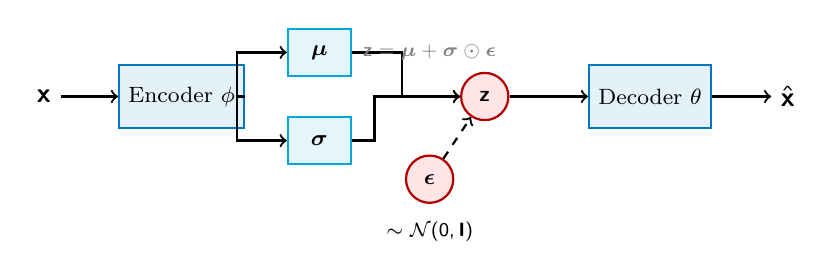
\begin{tikzpicture}[
    scale=0.7,
    block/.style={rectangle, draw=tudelftblue, fill=tudelftblue!10, thick, minimum width=1.5cm, minimum height=0.8cm, font=\footnotesize},
    param/.style={rectangle, draw=tudelftcyan, fill=tudelftcyan!10, thick, minimum width=0.8cm, minimum height=0.6cm, font=\footnotesize},
    sample/.style={circle, draw=red!70!black, fill=red!10, thick, minimum size=0.6cm, font=\footnotesize},
    arrow/.style={->, thick}
]
    % Input
    \node (x) at (0, 0) {$\mathbf{x}$};
    
    % Encoder
    \node[block] (enc) at (2.5, 0) {Encoder $\phi$};
    
    % Mu and Sigma
    \node[param] (mu) at (5, 0.8) {$\boldsymbol{\mu}$};
    \node[param] (sigma) at (5, -0.8) {$\boldsymbol{\sigma}$};
    
    % Epsilon
    \node[sample] (eps) at (7, -1.5) {$\boldsymbol{\epsilon}$};
    \node[font=\scriptsize, below=0.1cm of eps] {$\sim \mathcal{N}(0, \mathbf{I})$};
    
    % Z
    \node[sample] (z) at (8, 0) {$\mathbf{z}$};
    
    % Decoder
    \node[block] (dec) at (11, 0) {Decoder $\theta$};
    
    % Output
    \node (xhat) at (13.5, 0) {$\hat{\mathbf{x}}$};
    
    % Arrows
    \draw[arrow] (x) -- (enc);
    \draw[arrow] (enc) -- ++(1, 0) |- (mu);
    \draw[arrow] (enc) -- ++(1, 0) |- (sigma);
    \draw[arrow] (mu) -- ++(1.5, 0) |- (z);
    \draw[arrow] (sigma) -- ++(1, 0) |- (z);
    \draw[arrow, dashed] (eps) -- (z);
    \draw[arrow] (z) -- (dec);
    \draw[arrow] (dec) -- (xhat);
    
    % Reparameterization annotation
    \node[font=\scriptsize, text=gray] at (7, 0.8) {$\mathbf{z} = \boldsymbol{\mu} + \boldsymbol{\sigma} \odot \boldsymbol{\epsilon}$};
\end{tikzpicture}
\caption{VAE architecture with the reparameterization trick. The encoder outputs $\boldsymbol{\mu}$ and $\boldsymbol{\sigma}$. Sampling is done by $\mathbf{z} = \boldsymbol{\mu} + \boldsymbol{\sigma} \odot \boldsymbol{\epsilon}$, where $\boldsymbol{\epsilon}$ is external noise. This allows gradients to flow through $\boldsymbol{\mu}$ and $\boldsymbol{\sigma}$.}
\label{fig:vae}
\end{figure}

\subsection{Generative Adversarial Networks (GANs)}
GANs take a completely different approach: a \textbf{game} between two networks.
\begin{itemize}
	\item \textbf{Generator $G$:} Takes noise $\mathbf{z} \sim \mathcal{N}(0, \mathbf{I})$ and produces fake data $G(\mathbf{z})$. Its goal is to fool the discriminator.
	\item \textbf{Discriminator $D$:} Takes data (real or fake) and outputs the probability it's real. Its goal is to correctly classify real vs. fake.
\end{itemize}

\paragraph{The Minimax Objective:}
\begin{equation}
	\min_G \max_D \underbrace{\mathbb{E}_{\mathbf{x} \sim p_{\text{data}}}[\log D(\mathbf{x})]}_{\text{D wants this high (real $\to$ 1)}} + \underbrace{\mathbb{E}_{\mathbf{z} \sim p_z}[\log(1 - D(G(\mathbf{z})))]}_{\text{D wants this high (fake $\to$ 0), G wants it low}}
\end{equation}

\begin{figure}[H]
\centering
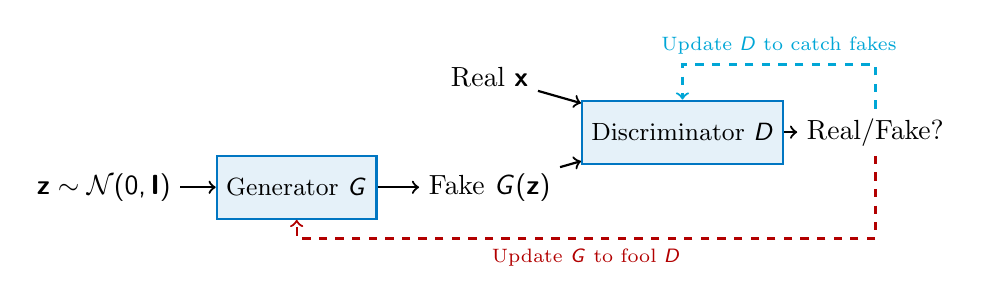
\begin{tikzpicture}[
    scale=0.7,
    block/.style={rectangle, draw=tudelftblue, fill=tudelftblue!10, thick, minimum width=2cm, minimum height=0.8cm, font=\small},
    arrow/.style={->, thick}
]
    % Noise
    \node (z) at (0, 0) {$\mathbf{z} \sim \mathcal{N}(0, \mathbf{I})$};
    
    % Generator
    \node[block] (G) at (3.5, 0) {Generator $G$};
    
    % Fake image
    \node (fake) at (7, 0) {Fake $G(\mathbf{z})$};
    
    % Real image
    \node (real) at (7, 2) {Real $\mathbf{x}$};
    
    % Discriminator
    \node[block] (D) at (10.5, 1) {Discriminator $D$};
    
    % Output
    \node (out) at (14, 1) {Real/Fake?};
    
    % Arrows
    \draw[arrow] (z) -- (G);
    \draw[arrow] (G) -- (fake);
    \draw[arrow] (fake) -- (D);
    \draw[arrow] (real) -- (D);
    \draw[arrow] (D) -- (out);
    
    % Feedback arrows
    \draw[arrow, red!70!black, dashed] (out.south) -- ++(0, -1.5) -| node[pos=0.25, below, font=\scriptsize] {Update $G$ to fool $D$} (G.south);
    \draw[arrow, tudelftcyan, dashed] (out.north) -- ++(0, 0.8) -| node[pos=0.25, above, font=\scriptsize] {Update $D$ to catch fakes} (D.north);
\end{tikzpicture}
\caption{GAN architecture. The generator transforms noise into fake data. The discriminator tries to distinguish real from fake. Training alternates between updating $D$ (to improve detection) and updating $G$ (to better fool $D$).}
\label{fig:gan}
\end{figure}

\paragraph{Training Challenges:}
\begin{itemize}
	\item \textbf{Mode collapse:} $G$ learns to produce only a few modes of the data distribution.
	\item \textbf{Unstable training:} Requires careful hyperparameter tuning.
	\item \textbf{No density estimation:} GANs don't give $p(\mathbf{x})$, only samples.
\end{itemize}
Despite challenges, GANs produce extremely \textbf{sharp, realistic images}.

\subsection{Diffusion Models}
Diffusion models (2020--present) are now state-of-the-art for image generation (DALL-E 2, Stable Diffusion, Midjourney). The idea: learn to \textbf{reverse a gradual noising process}.

\paragraph{Forward Process (Noising):}
Starting from data $\mathbf{x}_0$, gradually add Gaussian noise over $T$ steps:
\begin{equation}
	\mathbf{x}_t = \sqrt{1 - \beta_t} \cdot \mathbf{x}_{t-1} + \sqrt{\beta_t} \cdot \boldsymbol{\epsilon}, \quad \boldsymbol{\epsilon} \sim \mathcal{N}(0, \mathbf{I})
\end{equation}
After many steps, $\mathbf{x}_T \approx \mathcal{N}(0, \mathbf{I})$---pure noise.

\paragraph{Reverse Process (Denoising):}
A neural network learns to predict the noise added at each step:
\begin{equation}
	\mathbf{x}_{t-1} = \frac{1}{\sqrt{1 - \beta_t}} \left( \mathbf{x}_t - \frac{\beta_t}{\sqrt{1 - \bar{\alpha}_t}} \boldsymbol{\epsilon}_\theta(\mathbf{x}_t, t) \right) + \sigma_t \mathbf{z}
\end{equation}
where $\boldsymbol{\epsilon}_\theta$ is the learned noise predictor (often a U-Net). To generate, start with pure noise and iteratively denoise.

\begin{figure}[H]
\centering
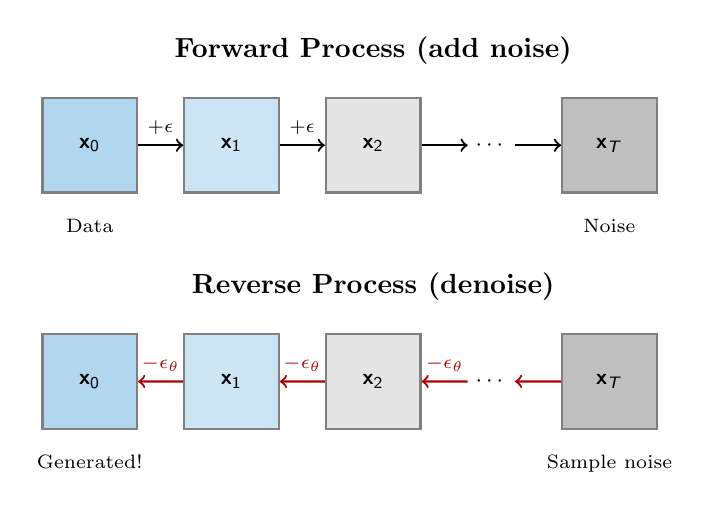
\begin{tikzpicture}[
    scale=0.6,
    img/.style={rectangle, draw=gray, thick, minimum width=1.2cm, minimum height=1.2cm, font=\footnotesize},
    arrow/.style={->, thick}
]
    % Forward process
    \node[font=\bfseries] at (6, 2) {Forward Process (add noise)};
    
    \node[img, fill=tudelftblue!30] (x0) at (0, 0) {$\mathbf{x}_0$};
    \node[img, fill=tudelftblue!20] (x1) at (3, 0) {$\mathbf{x}_1$};
    \node[img, fill=gray!20] (x2) at (6, 0) {$\mathbf{x}_2$};
    \node[font=\footnotesize] at (8.5, 0) {$\cdots$};
    \node[img, fill=gray!50] (xT) at (11, 0) {$\mathbf{x}_T$};
    
    \draw[arrow] (x0) -- node[above, font=\scriptsize] {$+\epsilon$} (x1);
    \draw[arrow] (x1) -- node[above, font=\scriptsize] {$+\epsilon$} (x2);
    \draw[arrow] (x2) -- (8, 0);
    \draw[arrow] (9, 0) -- (xT);
    
    \node[font=\scriptsize, below=0.2cm of x0] {Data};
    \node[font=\scriptsize, below=0.2cm of xT] {Noise};
    
    % Reverse process
    \node[font=\bfseries] at (6, -3) {Reverse Process (denoise)};
    
    \node[img, fill=gray!50] (xT2) at (11, -5) {$\mathbf{x}_T$};
    \node[font=\footnotesize] at (8.5, -5) {$\cdots$};
    \node[img, fill=gray!20] (x22) at (6, -5) {$\mathbf{x}_2$};
    \node[img, fill=tudelftblue!20] (x12) at (3, -5) {$\mathbf{x}_1$};
    \node[img, fill=tudelftblue!30] (x02) at (0, -5) {$\mathbf{x}_0$};
    
    \draw[arrow, red!70!black] (xT2) -- (9, -5);
    \draw[arrow, red!70!black] (8, -5) -- node[above, font=\scriptsize] {$-\epsilon_\theta$} (x22);
    \draw[arrow, red!70!black] (x22) -- node[above, font=\scriptsize] {$-\epsilon_\theta$} (x12);
    \draw[arrow, red!70!black] (x12) -- node[above, font=\scriptsize] {$-\epsilon_\theta$} (x02);
    
    \node[font=\scriptsize, below=0.2cm of xT2] {Sample noise};
    \node[font=\scriptsize, below=0.2cm of x02] {Generated!};
\end{tikzpicture}
\caption{Diffusion models. \textbf{Forward:} Gradually add noise until data becomes pure Gaussian noise. \textbf{Reverse:} A neural network learns to predict and remove noise at each step, transforming noise back into data.}
\label{fig:diffusion}
\end{figure}

\paragraph{Why Diffusion Works:}
\begin{itemize}
	\item The network is essentially a \textbf{denoising autoencoder} trained at all noise levels.
	\item Training is stable (simple MSE loss on predicted noise).
	\item Produces high-quality, diverse samples without mode collapse.
\end{itemize}

\subsection{Comparison of Generative Models}
\begin{table}[H]
\centering
\begin{tblr}{
  colspec = {l l l l},
  row{1} = {font=\bfseries},
  hline{1,2,Z} = {solid},
}
Model & Training & Sample Quality & Density? \\
VAE & Stable (ELBO) & Blurry & Yes (approx) \\
GAN & Unstable (adversarial) & Sharp & No \\
Diffusion & Stable (denoising) & State-of-the-art & Yes (approx) \\
\end{tblr}
\caption{Comparison of major generative model families.}
\label{tab:generative_models}
\end{table}


\section{Foundation Models and Transfer Learning}
\label{sec:dl_foundation}

The Deep Learning revolution has culminated in the era of \textbf{Foundation Models}, which are large-scale models trained on vast, diverse datasets that can be \textbf{adapted} to a wide range of downstream tasks. This represents a fundamental paradigm shift:
\begin{center}
	\textit{From ``training a model \textbf{for} a task'' to ``adapting a general model \textbf{to} a task.''}
\end{center}

\subsection{The Rise of Foundation Models}
A foundation model is defined by three properties:
\begin{enumerate}
	\item \textbf{Scale:} Trained on internet-scale data (billions of tokens/images).
	\item \textbf{Generality:} Learns representations applicable to many tasks.
	\item \textbf{Adaptability:} Can be fine-tuned or prompted for specific applications.
\end{enumerate}

\paragraph{Emergence and Homogenization:}
Two striking phenomena characterize foundation models:
\begin{itemize}
	\item \textbf{Emergence:} Capabilities arise that were not explicitly trained for. GPT-3 can do arithmetic, write poetry, and translate languages, none of which were direct training objectives.
	\item \textbf{Homogenization:} The same Transformer architecture now dominates language, vision, audio, and multimodal tasks. This consolidation simplifies research but concentrates power in few large models.
\end{itemize}

\subsection{Vision Transformers (ViT)}
CNNs encode the inductive bias that nearby pixels are related (locality). Transformers have no such bias, they learn relationships globally from data. To apply Transformers to images:

\begin{tcolorbox}[colback=tudelftblue!5!white, colframe=tudelftblue, title=ViT Pipeline]
\begin{enumerate}
	\item \textbf{Patchify:} Split the image into non-overlapping patches (e.g., $16 \times 16$ pixels).
	\item \textbf{Flatten \& Project:} Each patch is flattened into a vector and linearly projected to the model dimension.
	\item \textbf{Add Position:} Add learnable positional embeddings (so the model knows spatial arrangement).
	\item \textbf{Prepend [CLS]:} A special classification token aggregates global information.
	\item \textbf{Transformer Encoder:} Process the sequence of patch embeddings with standard self-attention.
	\item \textbf{Classify:} Use the final [CLS] embedding for prediction.
\end{enumerate}
\end{tcolorbox}

\begin{figure}[H]
\centering
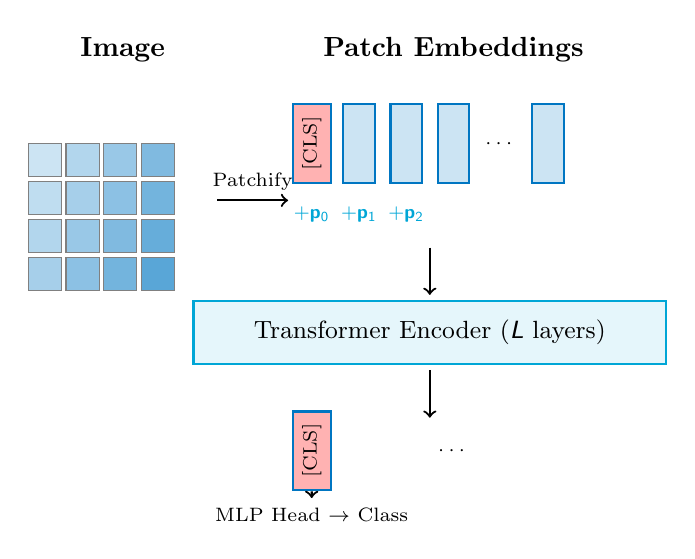
\begin{tikzpicture}[
    scale=0.6,
    patch/.style={rectangle, draw=gray, thick, minimum size=0.5cm},
    embed/.style={rectangle, draw=tudelftblue, fill=tudelftblue!20, thick, minimum width=0.4cm, minimum height=1cm, font=\scriptsize},
    block/.style={rectangle, draw=tudelftcyan, fill=tudelftcyan!10, thick, minimum width=6cm, minimum height=0.8cm, font=\small},
    arrow/.style={->, thick}
]
    % Image
    \node[font=\bfseries] at (2, 2) {Image};
    \foreach \i in {0,...,3} {
        \foreach \j in {0,...,3} {
            \fill[tudelftblue!\the\numexpr20+10*\i+5*\j\relax] (\i*0.8, -\j*0.8) rectangle (\i*0.8+0.7, -\j*0.8-0.7);
            \draw[gray] (\i*0.8, -\j*0.8) rectangle (\i*0.8+0.7, -\j*0.8-0.7);
        }
    }
    
    % Arrow
    \draw[arrow] (4, -1.2) -- (5.5, -1.2) node[midway, above, font=\scriptsize] {Patchify};
    
    % Patches as sequence
    \node[font=\bfseries] at (9, 2) {Patch Embeddings};
    \node[embed, fill=red!30] (cls) at (6, 0) {\rotatebox{90}{[CLS]}};
    \node[embed] (p1) at (7, 0) {};
    \node[embed] (p2) at (8, 0) {};
    \node[embed] (p3) at (9, 0) {};
    \node[font=\scriptsize] at (10, 0) {$\cdots$};
    \node[embed] (pn) at (11, 0) {};
    
    % Position embeddings
    \node[font=\scriptsize, text=tudelftcyan] at (6, -1.5) {$+\mathbf{p}_0$};
    \node[font=\scriptsize, text=tudelftcyan] at (7, -1.5) {$+\mathbf{p}_1$};
    \node[font=\scriptsize, text=tudelftcyan] at (8, -1.5) {$+\mathbf{p}_2$};
    
    % Arrow down
    \draw[arrow] (8.5, -2.2) -- (8.5, -3.2);
    
    % Transformer
    \node[block] (trans) at (8.5, -4) {Transformer Encoder ($L$ layers)};
    
    % Arrow down
    \draw[arrow] (8.5, -4.8) -- (8.5, -5.8);
    
    % Output
    \node[embed, fill=red!30] (out) at (6, -6.5) {\rotatebox{90}{[CLS]}};
    \node[font=\scriptsize] at (9, -6.5) {$\cdots$};
    
    % Classification
    \draw[arrow] (out.south) -- (6, -7.5) node[below, font=\scriptsize] {MLP Head $\to$ Class};
\end{tikzpicture}
\caption{Vision Transformer (ViT) architecture. The image is split into patches, each becomes a token. A [CLS] token aggregates global information through self-attention across all patches. Unlike CNNs, ViT has a global receptive field from layer 1.}
\label{fig:vit}
\end{figure}

\paragraph{ViT vs. CNN:}
\begin{itemize}
	\item \textbf{Inductive Bias:} CNNs assume locality (nearby pixels matter most). ViT has no such assumption, it must learn spatial relationships from data, requiring more training samples.
	\item \textbf{Scalability:} ViT scales better with data and compute. Given enough data, ViT outperforms CNNs.
	\item \textbf{Global Context:} ViT can attend to any patch from the first layer; CNNs need many layers to build large receptive fields.
\end{itemize}

\subsection{Self-Supervised Pre-Training}
The key to foundation models is \textbf{self-supervised learning}, which means defining training objectives that don't require human labels. The data provides its own supervision.

\begin{table}[H]
\centering
\begin{tblr}{
  colspec = {l l X[l]},
  row{1} = {font=\bfseries},
  hline{1,2,Z} = {solid},
}
Modality & Method & Pretext Task \\
Text & GPT (Autoregressive) & Predict the next token: ``The cat sat on the [?]'' \\
Text & BERT (Masked LM) & Fill in masked tokens: ``The [MASK] sat on the mat.'' \\
Images & MAE & Reconstruct 75\% masked image patches \\
Multimodal & CLIP & Match images and captions via contrastive loss \\
\end{tblr}
\caption{Self-supervised pre-training paradigms. Each defines a task where labels come from the data itself.}
\label{tab:ssl}
\end{table}

\paragraph{CLIP (Contrastive Language-Image Pre-training):}
Given $N$ (image, caption) pairs, CLIP learns to maximize the cosine similarity of matching pairs while minimizing it for the $N^2 - N$ non-matching pairs:
\begin{equation}
	\mathcal{L} = -\frac{1}{N} \sum_{i=1}^{N} \log \frac{\exp(\text{sim}(\mathbf{v}_i, \mathbf{t}_i) / \tau)}{\sum_{j=1}^{N} \exp(\text{sim}(\mathbf{v}_i, \mathbf{t}_j) / \tau)}
\end{equation}
where $\mathbf{v}_i$ and $\mathbf{t}_i$ are the image and text embeddings. This enables zero-shot classification: to classify an image, compute similarity to text prompts like ``a photo of a dog'' and pick the highest.

\subsection{Parameter-Efficient Fine-Tuning (PEFT)}
Fine-tuning a model with billions of parameters is computationally expensive and risks catastrophic forgetting. \textbf{PEFT} methods update only a tiny fraction of parameters while matching full fine-tuning performance.

\begin{tcolorbox}[colback=tudelftblue!5!white, colframe=tudelftblue, title=PEFT Strategies]
\textbf{1. Selective Fine-Tuning:} Freeze most layers, only train the last few layers or the classification head.

\textbf{2. Adapters:} Inject small trainable modules (bottleneck MLPs) into each layer:
\begin{equation}
	\text{Adapter}(\mathbf{x}) = \mathbf{W}_{\text{up}} \cdot \sigma(\mathbf{W}_{\text{down}} \cdot \mathbf{x}) + \mathbf{x}
\end{equation}
Typically $< 5\%$ additional parameters.

\textbf{3. Prompt Tuning:} Prepend learnable ``soft prompts'' (continuous vectors) to the input. The model parameters are frozen; only the prompts are trained.

\textbf{4. LoRA (Low-Rank Adaptation):} Add low-rank matrices that modify weight matrices without changing them:
\begin{equation}
	\mathbf{h} = \mathbf{W}_0 \mathbf{x} + \Delta\mathbf{W} \cdot \mathbf{x} = \mathbf{W}_0 \mathbf{x} + \mathbf{B}\mathbf{A}\mathbf{x}
\end{equation}
where $\mathbf{W}_0$ is frozen, $\mathbf{B} \in \mathbb{R}^{d \times r}$, $\mathbf{A} \in \mathbb{R}^{r \times k}$, and $r \ll \min(d, k)$.
\end{tcolorbox}

\begin{figure}[H]
\centering
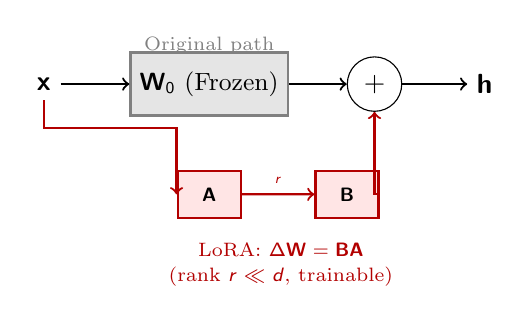
\begin{tikzpicture}[
    scale=0.7,
    block/.style={rectangle, draw=tudelftblue, fill=tudelftblue!10, thick, minimum width=2cm, minimum height=0.8cm, font=\small},
    frozen/.style={rectangle, draw=gray, fill=gray!20, thick, minimum width=2cm, minimum height=0.8cm, font=\small},
    lora/.style={rectangle, draw=red!70!black, fill=red!10, thick, minimum width=0.8cm, minimum height=0.6cm, font=\scriptsize},
    arrow/.style={->, thick}
]
    % Standard forward pass (frozen)
    \node (x) at (0, 0) {$\mathbf{x}$};
    \node[frozen] (W) at (3, 0) {$\mathbf{W}_0$ (Frozen)};
    \draw[arrow] (x) -- (W);
    
    % LoRA branch
    \node[lora] (A) at (3, -2) {$\mathbf{A}$};
    \node[lora] (B) at (5.5, -2) {$\mathbf{B}$};
    \draw[arrow, red!70!black] (x.south) -- ++(0, -0.5) -| (A.west);
    \draw[arrow, red!70!black] (A) -- node[above, font=\tiny] {$r$} (B);
    
    % Addition
    \node[circle, draw, fill=white, minimum size=0.4cm] (plus) at (6, 0) {$+$};
    \draw[arrow] (W) -- (plus);
    \draw[arrow, red!70!black] (B.east) -| (plus.south);
    
    % Output
    \node (h) at (8, 0) {$\mathbf{h}$};
    \draw[arrow] (plus) -- (h);
    
    % Annotations
    \node[font=\scriptsize, text=gray] at (3, 0.7) {Original path};
    \node[font=\scriptsize, text=red!70!black] at (4.3, -3) {LoRA: $\Delta\mathbf{W} = \mathbf{B}\mathbf{A}$};
    \node[font=\scriptsize, text=red!70!black] at (4.3, -3.5) {(rank $r \ll d$, trainable)};
\end{tikzpicture}
\caption{LoRA (Low-Rank Adaptation). The original weights $\mathbf{W}_0$ are frozen. A low-rank decomposition $\mathbf{B}\mathbf{A}$ is added in parallel and trained. This can reduce trainable parameters by 10,000$\times$ while matching full fine-tuning.}
\label{fig:lora}
\end{figure}

\end{document}
